\documentclass[dvips]{book}

\usepackage{makeidx}
\usepackage{index}
\usepackage[latin1]{inputenc}


\newcommand*{\indexuse}[1]{\hyperpage{#1}}
\newcommand*{\indexdef}[1]{\textbf{\hyperpage{#1}}}
\newcommand*{\indexsyn}[1]{\textbf{\textit{\hyperpage{#1}}}}

\begin{document}

\pagestyle{headings}
\pagestyle{empty}
\title{Global Constraint Catalog -- 2nd Edition}
\author{Nicolas Beldiceanu\thanks{Corresponding author, Email: \texttt{Nicolas.Beldiceanu@mines-nantes.fr},
�cole des Mines de Nantes,
LINA CNRS UMR 6241, 4 rue Alfred Kastler,
BP-20722, FR-44307~Nantes Cedex 3, France}}
\author{Mats Carlsson\thanks{SICS, Box 1263, SE-16~429~Kista, Sweden}}
\author{Jean-Xavier Rampon\thanks{LINA, 2 rue de la Houssini�re, BP-92208, FR-44322~Nantes Cedex 3, France}}

\reference{Working version of SICS Technical Report T2010:07\\[2ex]
ISSN: 1100-3154\\[2ex]
ISRN: SICS-T--2010/07-SE}

\begin{abstract}
This report presents a catalogue of global constraints where each constraint is explicitly described in terms of graph properties and/or automata and/or first order logical formulae with arithmetic. When available, it also presents some typical usage as well as some pointers to existing filtering algorithms.
\end{abstract}

\keywords{constraint programming, global constraint, catalogue, graph, automaton, first order formula, meta-data, ontology, symmetry.}
\maketitle


\thispagestyle{empty}
\cleardoublepage
\setcounter{page}{1}
%%%%%%%%%%%%%%%%%%%%%%%%%%%%%%%%%%%%%%%%%%%%%%%%%%%%%%%%%%%%%%%%%%
\dominitoc
\makeatletter
\newenvironment{chapquote}[2][2em]
  {\setlength{\@tempdima}{#1}%
   \def\chapquote@author{#2}%
   \parshape 1 \@tempdima \dimexpr\textwidth-2\@tempdima\relax%
   \itshape}
  {\par\normalfont\hfill--\ \chapquote@author\hspace*{\@tempdima}\par\bigskip}
\renewcommand\l@section{\@dottedtocline{1}{1.1em}{3.6em}}
\renewcommand\l@subsection{\@dottedtocline{2}{1.1em}{3.6em}}
\renewcommand\l@subsubsection{\@dottedtocline{3}{1.1em}{3.6em}}
\renewcommand\l@paragraph{\@dottedtocline{4}{1.1em}{3.6em}}
\renewcommand\l@subparagraph{\@dottedtocline{5}{1.1em}{3.6em}}
\makeatother
\setcounter{minitocdepth}{5}
\tableofcontents
%%%%%%%%%%%%%%%%%%%%%%%%%%%%%%%%%%%%%%%%%%%%%%%%%%%%%%%%%%%%%%%%%%


\frontmatter
\chapter{Preface}

\begin{chapquote}{Douglas Hofstadter, Emmanuel Sander, \textit{Surfaces and Essences}}
``Although dictionaries give the impression of analyzing words all the way down to their very atoms, all they do in fact is graze their surfaces.''
\end{chapquote}

This catalogue presents a list of global constraints. Within this catalogue the term \emph{global constraint} should be understood as an \emph{expressive and concise condition involving a non\nobreakdash-fixed number of variables}. This informal definition does not make any assumption neither about the potential use of a global constraint nor about the techniques\footnote{As quoted by J.~N.~Hooker in\index{Hooker J. N.|indexuse}~\cite{Hooker07}, ``\emph{identifying a field with its techniques is an intellectually as well as practically unsatisfying}'' and has a lot of drawbacks.} associated with the development of global constraints. It contains about $423$ constraints, which are explicitly described in terms of graph properties and/or automata and/or first order logic formulae and/or conjunction of other constraints.

This \emph{Global Constraint Catalogue} is an expanded version of the list of global constraints presented in\index{Beldiceanu N.|indexuse}~\cite{BeldiceanuR00} and an updated version of\index{Beldiceanu N.|indexuse}\index{Carlsson M.|indexuse}\index{Rampon J.-X.|indexuse}~\cite{BeldiceanuCarlssonRampon05}. The principle used for describing global constraints has been slightly modified in order to deal with a larger number of global constraints. Since $2003$, we try to provide an automaton that recognises the solutions associated with a global constraint. Since $2009$, we also try to provide a first order logic formula for defining the solutions accepted by a geometrical constraint.

\paragraph{Use of the catalogue.}
The catalogue is organised into five chapters:
\begin{itemize}
\item
Chapter~\ref{chap:getting_started} provide a short overview of the main entries you may first consult when you are not familiar with the catalogue.

\item
Chapter~\ref{chap:describing_constraints} explains how the meaning of global constraints is described in terms of graph\nobreakdash-properties or in terms of automata. On the one hand, if one wants to consult the catalogue for getting the informal definition of a global constraint, examples of use of that constraint or pointers to filtering algorithms, then one only needs to read the first section of Chapter~\ref{chap:describing_constraints}: describing the arguments of a global constraint, page \pageref{sec:arguments}. On the other hand, if one wants to understand those entries describing explicitly the meaning of a constraint then all the material of Chapter~\ref{chap:describing_constraints} is required.

\item
Chapter~\ref{chap:describing_catalogue} describes the content of the catalogue as well as different ways for searching through the catalogue. This material is essential.

\item
Chapter~\ref{chap:further_topics} covers additional topics, such as the differences from the $2000$ report\index{Beldiceanu N.|indexuse}~\cite{BeldiceanuR00} on global constraints, the generation of implied constraints that are systematically linked to the graph\nobreakdash-based description of a global constraint, and the electronic version of the catalogue. The material describing the format of the entries of a global constraint is mandatory for those who want to exploit the electronic version in order to write pre\nobreakdash-processors for performing various tasks for a global constraint. 

\item
Finally, Chapter~\ref{chap:catalogue} corresponds to the catalogue itself, which gives the global constraints in alphabetical order.\\
\end{itemize}

\mainmatter
\chapter{Getting started}\label{chap:getting_started}

Within keywords and constraints, the icons
\begin{description}
\item[~~\bclampe] indicates a point of interest (e.g.,~a necessary condition, a typical use),
\item[~~\bcdz] denotes a typical error or a common misunderstanding.
\end{description}

\chapter{Describing Global Constraints}\label{chap:describing_constraints}

\minitoc

We first introduce the notion of global constraint as well as the different facets attached to global constraints. We then motivate the need for an explicit description of global constraints and then present the \emph{graph\nobreakdash-based} as well as the \emph{automaton\nobreakdash-based} descriptions used throughout the catalogue. On the one hand, the graph\nobreakdash-based representation considers a global constraint as a subgraph of an initial given graph. This subgraph has to satisfy a set of required graph properties. On the other hand, the automaton\nobreakdash-based representation denotes a global constraint as a hypergraph constructed from a given constraint checker.\footnote{A \emph{constraint checker} is a program that takes an instance of a constraint for which all variables are fixed and tests whether the constraint is satisfied or not.} Both, the initial graph of the graph\nobreakdash-based representation, as well as the hypergraph of the automaton\nobreakdash-based representation have a very regular structure, which should give the opportunity for efficient filtering algorithms taking advantage of this structure.

\chapter{Description of the Catalogue}\label{chap:describing_catalogue}

\minitoc

\section{Which global constraints are included?}

The global constraints of this catalogue come from the following sources:
\begin{itemize}
\item
Existing constraint systems like:
  \begin{itemize}
  \item
  \index{ALICE|indexdef}ALICE\index{Lauri\`ere J.-L.|indexuse}~\cite{Lauriere78},
  \item
  \index{CHARME|indexdef}CHARME in C\index{Oplobedu A.|indexuse}\index{Marcovitch J.|indexuse}\index{Tourbier Y.|indexuse}~\cite{OplobeduMarcovitchTourbier89},
  \item
  \index{CHIP|indexdef}\href{http://www.cosytec.com}{{\bf CHIP}}\index{Dincbas M.|indexuse}\index{Van Hentenryck P.|indexuse}\index{Simonis H.|indexuse}\index{Aggoun A.|indexuse}\index{Graf T.|indexuse}\index{Berthier F.|indexuse}~\cite{DincbasVanHentenryckSimonisAggounGrafBerthier88} in Prolog, C and C++\ \
  ({\footnotesize \url{http://www.cosytec.com}}),
  \item
  \index{Choco|indexdef}\href{http://choco.emn.fr/}{{\bf Choco}}\index{Laburthe F.|indexuse}~\cite{Laburthe00} in Java\ \
  ({\footnotesize \url{http://choco.emn.fr/}}),
  \item
  \index{ECLAIR|indexdef}ECLAIR~\cite{Platon03} in Claire,
  \item
  \index{ECLiPSe|indexdef}\href{http://eclipseclp.org/}{{\bf ECLiPSe}}\index{Cheadle A. M.|indexuse}\index{Harvey W.|indexuse}\index{Sadler A. J.|indexuse}\index{Schimpf J.|indexuse}\index{Shen K.|indexuse}\index{Apt K. R.|indexuse}\index{Wallace M. G.|indexuse}~\cite{ECLiPSe03,AptWallace07} in Prolog\ \
  ({\footnotesize \url{http://eclipseclp.org/}}),
  \item
  \index{FaCile|indexdef}\href{http://www.recherche.enac.fr/opti/facile/}{{\bf FaCile}} in OCaml\ \
  ({\footnotesize \url{http://www.recherche.enac.fr/opti/facile/}}),
  \item
  \index{Gecode|indexdef}\href{http://www.gecode.org/}{{\bf Gecode}} in C++~\cite{Gecode06}\ \
  ({\footnotesize \url{http://www.gecode.org/}}),
  \item
  \index{SICStus|indexdef}\href{http://www.sics.se/sicstus/}{{\bf SICStus}}\index{Carlsson M.|indexuse}\index{Ottosson G.|indexuse}\index{Carlson B.|indexuse}~\cite{CarlssonOttossonCarlson97} in Prolog\ \
  ({\footnotesize \url{http://www.sics.se/sicstus/}}).
  \end{itemize}
  When available, the {\bf Systems} slot of a global constraint entry of the catalogue
  provides the name of the corresponding global constraint
  in the context of the
  \index{Choco|indexuse}\href{http://choco.emn.fr/}{{\bf Choco}},
  \index{Gecode|indexuse}\href{http://www.gecode.org/}{{\bf Gecode}},
  \index{JaCoP|indexuse}\href{http://www.jacop.eu/}{{\bf JaCoP}},
  \index{MiniZinc|indexuse}\href{http://www.minizinc.org/}{{\bf MiniZinc}}, and
  \index{SICStus|indexuse}\href{http://www.sics.se/sicstus/}{{\bf SICStus}} systems.
\item
Constraint programming articles mostly from conferences like:
  \begin{itemize}
  \item
  The Principles and Practice of Constraint Programming (CP)\\
  ({\footnotesize \url{http://www.informatik.uni-trier.de/~ley/db/conf/cp/index.html}}),
  \item
  The International Joint Conference on Artificial Intelligence (IJCAI)\\
  ({\footnotesize \url{http://www.informatik.uni-trier.de/~ley/db/conf/ijcai/index.html}}),
  \item
  The National Conference on Artificial Intelligence (AAAI)\\
  ({\footnotesize \url{http://www.informatik.uni-trier.de/~ley/db/conf/aaai/index.html}}),
  \item
  The International Conference on Logic Programming (ICLP)\\
  ({\footnotesize \url{http://www.informatik.uni-trier.de/~ley/db/conf/iclp/index.html}}),
  \item
  The International Conference of AI and OR Techniques in Constraint Programming for Combinatorial Optimisation
  Problems (CPAIOR)\\
  ({\footnotesize \url{http://www.informatik.uni-trier.de/~ley/db/conf/cpaior/}}).
  \end{itemize}

\item
Graph constraints from the CP(Graph) computation domain\index{Dooms G.|indexuse}~\cite{Dooms06}.

\item
New constraints inspired by variations of existing constraints, practical applications, combinatorial problems, puzzles or discussions with colleagues. 

\end{itemize}


\section{Which global constraints are missing?}

Constraints with too many arguments (like for instance the original \hyperlink{Ccycle}{\ctrref{cycle}}~\cite{Cosytec97} constraint with $16$ arguments), which are in fact a combination of several constraints, were not directly put into the catalogue. Constraints that have complex arguments were also omitted. Beside this, the following constraints should be added in some future version of the catalogue:
\ctrref{alldifferent\_on\_multisets}\index{Quimper C.-G.|indexuse}\index{Walsh T.|indexuse}~\cite{QuimperWalsh05}~\cite{QuimperWalshReport05},
\ctrref{case}\index{Carlsson M.|indexuse}~\cite{Sicstus95,Carlsson06},\index{Cheng K. C.K.|indexuse}\index{Yap R. H.C.|indexuse}~\cite{ChengYap05,ChengYap06},
\ctrref{choquet}\index{Le~Hu\'ed\'e F.|indexuse}\index{Grabisch M.|indexuse}\index{Labreuche C.|indexuse}\index{Sav\'eant P.|indexuse}~\cite{LeHuedeGrabischLabreucheSaveant06},
\ctrref{cost\_regular}\index{Demassey S.|indexuse}\index{Pesant G.|indexuse}\index{Rousseau L.-M.|indexuse}~\cite{DemasseyPesantRousseau06},
\ctrref{cumulative\_trapeze}\index{Poder E.|indexuse}\index{Beldiceanu N.|indexuse}\index{Sanlaville E.|indexuse}~\cite{PoderBeldiceanuSanlaville04,BeldiceanuPoderPMS04}.
Finally we only consider a restricted number of constraints involving set variables since this is a relatively new area, which is currently growing rapidly since $2003$.

\chapter{Further Topics}\label{chap:further_topics}

\minitoc

\section{Differences from the 2000 report}

This section summarises the main differences with the SICS report\index{Beldiceanu N.|indexuse}~\cite{Beldiceanu00} as well as of the corresponding article\index{Beldiceanu N.|indexuse}~\cite{BeldiceanuR00}.

\chapter{Global Constraint Catalogue}\label{chap:catalogue}
\minitoc
\pagestyle{myheadings}
\cleardoublepageeven
\section{alldifferent}
\hypertarget{Calldifferent}{}
\sbox{\signbox}{\small$\underline{\graphproperty{MAX\_NSCC}},\arcgenerator{CLIQUE}$}
\index{signature!MAX\_NSCCCLIQUE@\small$\underline{\graphproperty{MAX\_NSCC}},\arcgenerator{CLIQUE}$!alldifferent@$\constraint{alldifferent}$|indexuse}
\markboth{\usebox{\signbox}}{20000128}
\def\MVARIABLES{\argument{VARIABLES}}
\def\Malldifferent{\argument{alldifferent}}
\def\MMAXNSCC{\graphproperty{MAX\_NSCC}}
\def\Mvar{\argument{var}}
\def\MSORTEDVARIABLES{\argument{SORTED\_VARIABLES}}
\def\examplefig{}
\def\examplefigv{}
\begin{tabular}{l@{\hspace{.15\textwidth}}l@{\hspace{.15\textwidth}}l@{\hspace{.15\textwidth}}l}
\bf \hyperlink{CalldifferentPdesc}{DESCRIPTION} & \bf \hyperlink{CalldifferentPlinks}{LINKS} & \bf \hyperlink{CalldifferentPgraph}{GRAPH} & \bf \hyperlink{CalldifferentPauto}{AUTOMATON} \\
\end{tabular}
\begin{ctrdesc}
\index{Lauri\`ere J.-L.|indexuse}
\index{Costa M.-C.|indexuse}
\index{R\'egin J.-C.|indexuse}
\index{Petersen J.|indexuse}
\index{Berge C.|indexuse}
\index{Leconte M.|indexuse}
\index{Bleuzen-Guernalec N.|indexuse}
\index{Colmerauer A.|indexuse}
\index{Puget J.-F.|indexuse}
\index{L\'opez-Ortiz A.|indexuse}
\index{Quimper C.-G.|indexuse}
\index{van Beek P.|indexuse}
\index{Mehlhorn K.|indexuse}
\index{Thiel S.|indexuse}
\index{van Hoeve W.-J.|indexuse}
\index{Glover F.|indexuse}
\index{Asratian A. S.|indexuse}
\index{Denley T. M. J.|indexuse}
\index{H\"aggkvist R.|indexuse}
\index{Williams H. P.|indexuse}
\index{Yan H.|indexuse}
\index{Hooker J. N.|indexuse}
\index{Zanarini A.|indexuse}
\index{Pesant G.|indexuse}
\index{Valiant L. G.|indexuse}
\index{Sloane N. J. A.|indexuse}
\index{Gent I. P.|indexuse}
\index{Nightingale P.|indexuse}
\index{Vellino A.|indexuse}
\index{Bron C.|indexuse}
\index{Kerbosch J.|indexuse}
\index{Eppstein D.|indexuse}
\index{Strash D.|indexuse}
\index{Bessi\`ere C.|indexuse}
\index{Katsirelos G.|indexuse}
\index{Narodytska N.|indexuse}
\index{Walsh T.|indexuse}
\index{Rochart G.|indexuse}
\index{Jussien N.|indexuse}
\index{Barichard V.|indexuse}
\index{Roy B.|indexuse}
\index{Watkins J. J.|indexuse}
\index{Gauss K. F.|indexuse}
\index{D\"urr C.|indexuse}
\index{Cymer R.|indexuse}
\index{alldifferent@$\constraint{alldifferent}$|indexdef}
\item[\pdfmarkup{subject={Origin},color=white,markup=Highlight}{Origin}{The origin of the constraint: reference to a paper, to a person, to an other constraint or to a system.}]
\hypertarget{CalldifferentPdesc}{}
\cite{Lauriere78}
\item[\pdfmarkup{subject={Constraint},color=white,markup=Highlight}{Constraint}{The constraint name and its arguments.}]
\colorbox{MyAzurelight}{\begin{minipage}[t]{11.2cm}
$\constraint{alldifferent}(\argument{VARIABLES})$
\end{minipage}}
\item[\pdfmarkup{subject={Synonyms},color=white,markup=Highlight}{Synonyms}{List of synonyms for the name of the constraint.}]
\colorbox{MyAzurelight}{\begin{minipage}[t]{11.2cm}
$\constraint{alldiff}$,\hfil
\index{alldiff@$\constraint{alldiff}$|indexsyn}
$\constraint{alldistinct}$,\hfil
\index{alldistinct@$\constraint{alldistinct}$|indexsyn}
$\constraint{distinct}$,\hfil
\index{distinct@$\constraint{distinct}$|indexsyn}
$\constraint{bound\_alldifferent}$,\hfil
\index{bound\_alldifferent@$\constraint{bound\_alldifferent}$|indexsyn}
$\constraint{bound\_alldiff}$,\hfil
\index{bound\_alldiff@$\constraint{bound\_alldiff}$|indexsyn}
$\constraint{bound\_distinct}$,\hfil
\index{bound\_distinct@$\constraint{bound\_distinct}$|indexsyn}
$\constraint{rel}$.\hfill
\index{rel@$\constraint{rel}$|indexsyn}

\end{minipage}}
\item[\pdfmarkup{subject={Argument},color=white,markup=Highlight}{Argument}{Argument of the constraint and its corresponding type.}]
\colorbox{MyAzurelight}{\begin{minipage}[t]{11.2cm}
\begin{tabular}[t]{l@{\quad:\quad}l}
$\argument{VARIABLES}$ & $ $\hyperlink{DT_collection}{$\argument{collection}$}$ (\argument{var}- $\hyperlink{DT_dvar}{$\argument{dvar}$}$ )$ \\
\end{tabular}

\end{minipage}}
\item[\pdfmarkup{subject={Restriction},color=white,markup=Highlight}{Restriction}{Additional condition refining the type declarations of one or several arguments of the constraint.}]
\colorbox{MyAzurelight}{\begin{minipage}[t]{11.2cm}
\begin{tabular}[t]{l}
$ $\hyperlink{PR_required}{$\argument{required}$}$ (\argument{VARIABLES},\argument{var})$\\
\end{tabular}

\end{minipage}}
\item[\pdfmarkup{subject={Purpose},color=white,markup=Highlight}{Purpose}{Definition in natural language of the meaning of the constraint.}]
{\setlength\fboxrule{1.5pt}\fcolorbox{MyRed}{white}{\begin{minipage}{11.1cm}
Enforce all variables of the collection $\MVARIABLES$ to take distinct values.

\end{minipage}}}
\medskip
\def\examplefig{\examplefigiih{fig:alldifferent}{Initial and final graph of the \ctrrefself{alldifferent} constraint}{ctrs/alldifferentA}{ctrs/alldifferentB}}
\def\examplefigv{\examplefigiiv{fig:alldifferent}{Initial and final graph of the \ctrrefself{alldifferent} constraint}{ctrs/alldifferentA}{ctrs/alldifferentB}}
\item[\pdfmarkup{subject={Example},color=white,markup=Highlight}{Example}{One or several examples of ground solutions of the constraint.}]
{\setlength\fboxrule{1.5pt}\fcolorbox{MyCornflowerBlue}{MyYellowlight}{\makebox[\width]{
\begin{tabular}[t]{l}
$\argument{}(\left\langle5,1,9,3\right\rangle)$\\
\end{tabular}

}}}
\\\ \\
The \ctrrefself{alldifferent} constraint holds since all the values $5$, $1$, $9$ and $3$
are distinct.

\item[\pdfmarkup{subject={All solutions},color=white,markup=Highlight}{All solutions}{Example of all solutions for a non ground instance of the constraint.}]
Figure~\ref{fig:alldifferent0} gives all solutions to the following non ground instance of the \ctrrefself{alldifferent} constraint:
$V_1\in [2,4]$, $V_2\in [2,3]$, $V_3\in [1,6]$, $V_4\in [2,5]$, $V_5\in [2,3]$, $V_6\in [1,6]$,
\ctrrefself{alldifferent}$(\langle V_1,V_2,V_3,V_4,V_5,V_6\rangle)$.
\begin{figure}[!h]
\centering
{\small
\begin{tikzpicture}[every node/.style={single arrow, single arrow tip angle=135, single arrow head extend=1cm, draw=MyCornflowerBlue, line width=2pt}] \node [fill=MyYellowlight, single arrow, shape border rotate=270, text width=2.78 cm]
{\ding{172} $(\langle 4, 2, 1, 5, 3, 6\rangle)$\\
\ding{173} $(\langle 4, 2, 6, 5, 3, 1\rangle)$\\
\ding{174} $(\langle 4, 3, 1, 5, 2, 6\rangle)$\\
\ding{175} $(\langle 4, 3, 6, 5, 2, 1\rangle)$};
\end{tikzpicture}
\caption{\label{fig:alldifferent0}
All solutions corresponding to the non ground example of the \ctrrefself{alldifferent} constraint of the {\bf All solutions} slot}
}
\end{figure}

\item[\pdfmarkup{subject={Typical},color=white,markup=Highlight}{Typical}{Typical condition on the arguments of the constraint.}]
\colorbox{MyAzurelight}{\begin{minipage}[t]{11.2cm}
\begin{tabular}[t]{l}
$|\argument{VARIABLES}|>2$\\
\end{tabular}

\end{minipage}}
\item[\pdfmarkup{subject={Symmetries},color=white,markup=Highlight}{Symmetries}{List of mappings (e.g., permutation of arguments, permutation of items, permutation of attributes, permutation of values, translation of attributes) that preserve the solutions of the constraint.}]
\colorbox{MyAzurelight}{\begin{minipage}[t]{11.2cm}
\begin{itemize}
\item
Items of $\argument{VARIABLES}$ are \hyperlink{AS_items}{permutable}.
\item
Two distinct values of $\argument{VARIABLES}.\argument{var}$ can be \hyperlink{AS_vals}{swapped}; a value of $\argument{VARIABLES}.\argument{var}$ can be \hyperlink{AS_vals}{renamed} to any unused value.
\end{itemize}

\end{minipage}}
\item[\pdfmarkup{subject={Arg. properties},color=white,markup=Highlight}{Arg. properties}{Properties of some arguments of the constraint (e.g. Functional dependency: an argument is determined by some other arguments, Contractibility: can remove items from any position of a collection, Prefix-contractibility: can remove items from first position, Suffix-contractibility: can remove items from last position, Extensibility: can add items at any position of a collection, Prefix-extensibility: can add items before first position, Suffix-extensibility: can add items after last position).}]
\colorbox{MyAzurelight}{\begin{minipage}[t]{11.2cm}
\hyperlink{contractible}{Contractible} wrt. $\argument{VARIABLES}$.
\end{minipage}}
\item[\pdfmarkup{subject={Usage},color=white,markup=Highlight}{Usage}{Typical usage of the constraint.}]
The \ctrrefself{alldifferent} constraint occurs in most practical problems
directly or indirectly. A classical example is the \hyperlink{n-queens}{n-queens}
chess puzzle problem:
Place $n$ queens on an $n$ by $n$ chessboard in such a way that no
queen attacks another. Two queens attack each other if they are
located on the same column, on the same row, or on the same diagonal.
This can be modelled as the conjunction of three
\ctrrefself{alldifferent} constraints.
We associate to column $i$ of the chessboard a domain
variable $X_i$ that gives the row number where the corresponding
queen is located. The three \ctrrefself{alldifferent} constraints are:
\begin{itemize}
\item
$\Malldifferent(X_1    ,X_2+1  ,\dots,X_n+n-1)$ for the descending diagonals,
\item
$\Malldifferent(X_1    ,X_2    ,\dots,X_n    )$ for the rows,
\item
$\Malldifferent(X_1+n-1,X_2+n-2,\dots,X_n    )$ for the ascending diagonals.
\end{itemize}
They are respectively depicted by parts~(A), (C) and (D) of Figure~\ref{fig:alldifferent2}.
Figure~\ref{fig:alldifferent2a} makes explicit the link between the two families of diagonals
and the corresponding \ctrrefself{alldifferent} constraints.
Note that this model matches the checker introduced by Gauss to test whether a permutation
of row numbers is a solution or not to the $8$ queens problem: first add the numbers $1$ up to $8$ to the
permutation and check that the resulting numbers are distinct, second add the numbers $8$
down to $1$ and perform the same check~\cite[pages 165--166]{Watkins04}.

\begin{figure}[!h]
\centering
\begin{tikzpicture}[scale=0.4]
\begin{scope}[xshift=0cm,yshift=0cm]
\draw[color=black,thick] (-0.18,-0.18) rectangle (8.18,8.18);
\foreach \x in {0,1,2,3} \foreach \y in {0,1,2,3} \fill [gray!60] (2*\x,2*\y) rectangle (2*\x+1,2*\y+1);
\foreach \x in {0,1,2,3} \foreach \y in {0,1,2,3} \fill [gray!60] (2*\x+1,2*\y+1) rectangle (2*\x+2,2*\y+2);
\foreach \x in {1,2,3,4,5,6,7,8}
\draw[MyLightBlue!90,line width=0.6mm] (\x-0.2,0+0.2) -- (0+0.2,\x-0.2);
\foreach \x in {1,2,3,4,5,6,7}
\draw[MyLightBlue!90,line width=0.6mm] (8-0.2,\x+0.2) -- (\x+0.2,8-0.2);
\filldraw[fill=yellow, draw=black] (2,0) rectangle (3,1);
\filldraw[fill=red, draw=black] (1,2) rectangle (2,3);
\filldraw[fill=blue!35, draw=black] (0,4) rectangle (1,5);
\filldraw[fill=MyOrange, draw=black] (4,1) rectangle (5,2);
\filldraw[fill=MyPineGreen!50, draw=black] (3,6) rectangle (4,7);
\filldraw[fill=MyRhodamine, draw=black] (7,3) rectangle (8,4);
\filldraw[fill=MyChartreuse, draw=black] (6,5) rectangle (7,6);
\filldraw[fill=MyRedOrange, draw=black] (5,7) rectangle (6,8);
\draw (0.5,4.5) node{{\large\figsymbol{Q}}};
\draw (1.5,2.5) node{{\large\figsymbol{Q}}};
\draw (2.5,0.5) node{{\large\figsymbol{Q}}};
\draw (3.5,6.5) node{{\large\figsymbol{Q}}};
\draw (4.5,1.5) node{{\large\figsymbol{Q}}};
\draw (5.5,7.5) node{{\large\figsymbol{Q}}};
\draw (6.5,5.5) node{{\large\figsymbol{Q}}};
\draw (7.5,3.5) node{{\large\figsymbol{Q}}};
\draw (0,0) grid (8,8);
\foreach \x in {1,2,3,4,5,6,7,8}
\coordinate [label=left:{\scriptsize$X_{\x}$}] (X) at (\x+0.25,-0.75);
\foreach \x in {1,2,3,4,5,6,7,8}
\coordinate [label=left:{\scriptsize$\x$}] (X) at (-0.25,\x-0.5);
\draw (4,-2) node{\small(A)};
\end{scope}
\begin{scope}[xshift=11.5cm,yshift=0cm]
\draw[color=black,thick] (-0.18,-0.18) rectangle (8.18,8.18);
\foreach \x in {0,1,2,3} \foreach \y in {0,1,2,3} \fill [gray!60] (2*\x,2*\y) rectangle (2*\x+1,2*\y+1);
\foreach \x in {0,1,2,3} \foreach \y in {0,1,2,3} \fill [gray!60] (2*\x+1,2*\y+1) rectangle (2*\x+2,2*\y+2);
\foreach \x in {0,1,2,3,4,5,6,7}
\draw[black!70,line width=0.6mm] (0+0.2,\x+0.5) -- (8.0-0.2,\x+0.5);
\filldraw[fill=yellow, draw=black] (2,0) rectangle (3,1);
\filldraw[fill=red, draw=black] (1,2) rectangle (2,3);
\filldraw[fill=blue!35, draw=black] (0,4) rectangle (1,5);
\filldraw[fill=MyOrange, draw=black] (4,1) rectangle (5,2);
\filldraw[fill=MyPineGreen!50, draw=black] (3,6) rectangle (4,7);
\filldraw[fill=MyRhodamine, draw=black] (7,3) rectangle (8,4);
\filldraw[fill=MyChartreuse, draw=black] (6,5) rectangle (7,6);
\filldraw[fill=MyRedOrange, draw=black] (5,7) rectangle (6,8);
\draw (0.5,4.5) node{{\large\figsymbol{Q}}};
\draw (1.5,2.5) node{{\large\figsymbol{Q}}};
\draw (2.5,0.5) node{{\large\figsymbol{Q}}};
\draw (3.5,6.5) node{{\large\figsymbol{Q}}};
\draw (4.5,1.5) node{{\large\figsymbol{Q}}};
\draw (5.5,7.5) node{{\large\figsymbol{Q}}};
\draw (6.5,5.5) node{{\large\figsymbol{Q}}};
\draw (7.5,3.5) node{{\large\figsymbol{Q}}};
\draw (0,0) grid (8,8);
\foreach \x in {1,2,3,4,5,6,7,8}
\coordinate [label=left:{\scriptsize$X_{\x}$}] (X) at (\x+0.25,-0.75);
\foreach \x in {1,2,3,4,5,6,7,8}
\coordinate [label=left:{\scriptsize$\x$}] (X) at (-0.25,\x-0.5);
\draw (4,-2) node{\small(C)};
\end{scope}
\begin{scope}[xshift=23cm,yshift=0cm]
\draw[color=black,thick] (-0.18,-0.18) rectangle (8.18,8.18);
\foreach \x in {0,1,2,3} \foreach \y in {0,1,2,3} \fill [gray!60] (2*\x,2*\y) rectangle (2*\x+1,2*\y+1);
\foreach \x in {0,1,2,3} \foreach \y in {0,1,2,3} \fill [gray!60] (2*\x+1,2*\y+1) rectangle (2*\x+2,2*\y+2);
\foreach \x in {0,1,2,3,4,5,6,7}
\draw[pink,line width=0.6mm] (\x+0.2,0+0.2) -- (8-0.2,8-\x-0.2);
\foreach \x in {1,2,3,4,5,6,7}
\draw[pink,line width=0.6mm] (0+0.2,\x+0.2) -- (8-\x-0.2,8-0.2);
\filldraw[fill=yellow, draw=black] (2,0) rectangle (3,1);
\filldraw[fill=red, draw=black] (1,2) rectangle (2,3);
\filldraw[fill=blue!35, draw=black] (0,4) rectangle (1,5);
\filldraw[fill=MyOrange, draw=black] (4,1) rectangle (5,2);
\filldraw[fill=MyPineGreen!50, draw=black] (3,6) rectangle (4,7);
\filldraw[fill=MyRhodamine, draw=black] (7,3) rectangle (8,4);
\filldraw[fill=MyChartreuse, draw=black] (6,5) rectangle (7,6);
\filldraw[fill=MyRedOrange, draw=black] (5,7) rectangle (6,8);
\draw (0.5,4.5) node{{\large\figsymbol{Q}}};
\draw (1.5,2.5) node{{\large\figsymbol{Q}}};
\draw (2.5,0.5) node{{\large\figsymbol{Q}}};
\draw (3.5,6.5) node{{\large\figsymbol{Q}}};
\draw (4.5,1.5) node{{\large\figsymbol{Q}}};
\draw (5.5,7.5) node{{\large\figsymbol{Q}}};
\draw (6.5,5.5) node{{\large\figsymbol{Q}}};
\draw (7.5,3.5) node{{\large\figsymbol{Q}}};
\draw (0,0) grid (8,8);
\foreach \x in {1,2,3,4,5,6,7,8}
\coordinate [label=left:{\scriptsize$X_{\x}$}] (X) at (\x+0.25,-0.75);
\foreach \x in {1,2,3,4,5,6,7,8}
\coordinate [label=left:{\scriptsize$\x$}] (X) at (-0.25,\x-0.5);
\draw (4,-2) node{\small(D)};
\end{scope}
\begin{scope}[xshift=0cm,yshift=9cm]
\foreach \y in {0}
\filldraw[fill=gray!60, draw=black] (0,\y) rectangle (1,\y+1);
\foreach \y in {0,1}
\filldraw[fill=white, draw=black] (1,\y) rectangle (2,\y+1);
\foreach \y in {0,1,2}
\filldraw[fill=gray!60, draw=black] (2,\y) rectangle (3,\y+1);
\foreach \y in {0,1,2,3}
\filldraw[fill=white, draw=black] (3,\y) rectangle (4,\y+1);
\foreach \y in {0,1,2,3,4}
\filldraw[fill=gray!60, draw=black] (4,\y) rectangle (5,\y+1);
\foreach \y in {0,1,2,3,4,5}
\filldraw[fill=white, draw=black] (5,\y) rectangle (6,\y+1);
\foreach \y in {0,1,2,3,4,5,6}
\filldraw[fill=gray!60, draw=black] (6,\y) rectangle (7,\y+1);
\foreach \y in {0,1,2,3,4,5,6,7}
\filldraw[fill=white, draw=black] (7,\y) rectangle (8,\y+1);
\foreach \y in {1,2,3,4,5,6,7}
\filldraw[fill=gray!60, draw=black] (8,\y) rectangle (9,\y+1);
\foreach \y in {2,3,4,5,6,7}
\filldraw[fill=white, draw=black] (9,\y) rectangle (10,\y+1);
\foreach \y in {3,4,5,6,7}
\filldraw[fill=gray!60, draw=black] (10,\y) rectangle (11,\y+1);
\foreach \y in {4,5,6,7}
\filldraw[fill=white, draw=black] (11,\y) rectangle (12,\y+1);
\foreach \y in {5,6,7}
\filldraw[fill=gray!60, draw=black] (12,\y) rectangle (13,\y+1);
\foreach \y in {6,7}
\filldraw[fill=white, draw=black] (13,\y) rectangle (14,\y+1);
\foreach \y in {7}
\filldraw[fill=gray!60, draw=black] (14,\y) rectangle (15,\y+1);
\foreach \x in {0,1,2,3,4,5,6,7}
\draw[MyLightBlue!90,line width=0.6mm] (\x+0.5,0.2) -- (\x+0.5,\x+1-0.2);
\foreach \x in {1,2,3,4,5,6,7}
\draw[MyLightBlue!90,line width=0.6mm] (\x+7.5,\x+0.2) -- (\x+7.5,8-0.2);
\filldraw[fill=yellow, draw=black] (2,0) rectangle (3,1);
\filldraw[fill=red, draw=black] (3,2) rectangle (4,3);
\filldraw[fill=blue!35, draw=black] (4,4) rectangle (5,5);
\filldraw[fill=MyOrange, draw=black] (5,1) rectangle (6,2);
\filldraw[fill=MyPineGreen!50, draw=black] (9,6) rectangle (10,7);
\filldraw[fill=MyRhodamine, draw=black] (10,3) rectangle (11,4);
\filldraw[fill=MyChartreuse, draw=black] (11,5) rectangle (12,6);
\filldraw[fill=MyRedOrange, draw=black] (12,7) rectangle (13,8);
\draw (2.5,0.5) node{{\large\figsymbol{Q}}};
\draw (3.5,2.5) node{{\large\figsymbol{Q}}};
\draw (4.5,4.5) node{{\large\figsymbol{Q}}};
\draw (5.5,1.5) node{{\large\figsymbol{Q}}};
\draw (9.5,6.5) node{{\large\figsymbol{Q}}};
\draw (10.5,3.5) node{{\large\figsymbol{Q}}};
\draw (11.5,5.5) node{{\large\figsymbol{Q}}};
\draw (12.5,7.5) node{{\large\figsymbol{Q}}};
\draw (2,5) node{\small(B)};
\end{scope}
\begin{scope}[xshift=16cm,yshift=9cm]
\foreach \y in {7}
\filldraw[fill=white, draw=black] (0,\y) rectangle (1,\y+1);
\foreach \y in {6,7}
\filldraw[fill=gray!60, draw=black] (1,\y) rectangle (2,\y+1);
\foreach \y in {5,6,7}
\filldraw[fill=white, draw=black] (2,\y) rectangle (3,\y+1);
\foreach \y in {4,5,6,7}
\filldraw[fill=gray!60, draw=black] (3,\y) rectangle (4,\y+1);
\foreach \y in {3,4,5,6,7}
\filldraw[fill=white, draw=black] (4,\y) rectangle (5,\y+1);
\foreach \y in {2,3,4,5,6,7}
\filldraw[fill=gray!60, draw=black] (5,\y) rectangle (6,\y+1);
\foreach \y in {1,2,3,4,5,6,7}
\filldraw[fill=white, draw=black] (6,\y) rectangle (7,\y+1);
\foreach \y in {0,1,2,3,4,5,6,7}
\filldraw[fill=gray!60, draw=black] (7,\y) rectangle (8,\y+1);
\foreach \y in {0,1,2,3,4,5,6}
\filldraw[fill=white, draw=black] (8,\y) rectangle (9,\y+1);
\foreach \y in {0,1,2,3,4,5}
\filldraw[fill=gray!60, draw=black] (9,\y) rectangle (10,\y+1);
\foreach \y in {0,1,2,3,4}
\filldraw[fill=white, draw=black] (10,\y) rectangle (11,\y+1);
\foreach \y in {0,1,2,3}
\filldraw[fill=gray!60, draw=black] (11,\y) rectangle (12,\y+1);
\foreach \y in {0,1,2}
\filldraw[fill=white, draw=black] (12,\y) rectangle (13,\y+1);
\foreach \y in {0,1}
\filldraw[fill=gray!60, draw=black] (13,\y) rectangle (14,\y+1);
\foreach \y in {0}
\filldraw[fill=white, draw=black] (14,\y) rectangle (15,\y+1);
\foreach \x in {0,1,2,3,4,5,6,7}
\draw[pink,line width=0.6mm] (\x+0.5,7-\x+0.2) -- (\x+0.5,8-0.2);
\foreach \x in {0,1,2,3,4,5,6}
\draw[pink,line width=0.6mm] (\x+8.5,0.2) -- (\x+8.5,7-\x-0.2);
\filldraw[fill=blue!35, draw=black] (3,4) rectangle (4,5);
\filldraw[fill=MyPineGreen!50, draw=black] (4,6) rectangle (5,7);
\filldraw[fill=red, draw=black] (5,7) rectangle (6,8);
\filldraw[fill=MyRedOrange, draw=black] (6,2) rectangle (7,3);
\filldraw[fill=MyChartreuse, draw=black] (8,5) rectangle (9,6);
\filldraw[fill=yellow, draw=black] (9,0) rectangle (10,1);
\filldraw[fill=MyOrange, draw=black] (10,1) rectangle (11,2);
\filldraw[fill=MyRhodamine, draw=black] (11,3) rectangle (12,4);
\draw (3.5,4.5) node{{\large\figsymbol{Q}}};
\draw (4.5,6.5) node{{\large\figsymbol{Q}}};
\draw (5.5,7.5) node{{\large\figsymbol{Q}}};
\draw (6.5,2.5) node{{\large\figsymbol{Q}}};
\draw (8.5,5.5) node{{\large\figsymbol{Q}}};
\draw (9.5,0.5) node{{\large\figsymbol{Q}}};
\draw (10.5,1.5) node{{\large\figsymbol{Q}}};
\draw (11.5,3.5) node{{\large\figsymbol{Q}}};
\draw (13,5) node{\small(E)};
\end{scope}
\end{tikzpicture}
\caption{\label{fig:alldifferent2}
Descending diagonals (A-B), rows (C) and ascending diagonals (D-E)}
\end{figure}

\begin{figure}[!h]
\centering
\begin{tikzpicture}[scale=0.4]
\begin{scope}
\draw[color=black,thick] (-0.18,-0.18) rectangle (8.18,8.18);
\foreach \x in {0,1,2,3} \foreach \y in {0,1,2,3} \fill [gray!60] (2*\x,2*\y) rectangle (2*\x+1,2*\y+1);
\foreach \x in {0,1,2,3} \foreach \y in {0,1,2,3} \fill [gray!60] (2*\x+1,2*\y+1) rectangle (2*\x+2,2*\y+2);
\foreach \x in {6} {
\draw[red,line width=0.6mm] (\x,1) -- (0+5,\x-6);
\draw[red,line width=0.6mm] (\x,0) -- (0+2,\x-2);
}
\foreach \x in {1} {
\draw[orange,line width=0.6mm] (0+2,\x+2) -- (8-\x-1,8-1);
\draw[orange,line width=0.6mm] (8-\x-1,8-2) -- (8-\x-2,8-1);
}
\filldraw[fill=yellow, draw=black] (2,3) rectangle (3,4);
\draw (2.5,3.5) node{{\large\figsymbol{Q}}};
\draw (0,0) grid (8,8);
\foreach \x/\t in {3/i,6/j}
\coordinate [label=left:{\scriptsize$\t$}] (X) at (\x-0.1,-0.75);
\foreach \x in {4}
\coordinate [label=left:{\scriptsize$X_i$}] (X) at (-0.25,\x-0.5);
\draw[>=stealth',shorten >=1pt,<->,densely dashed] (-0.75,4) -- (-0.75,7) node[midway,sloped,above] {\scriptsize$j-i$};
\draw[anchor=east] (-1.6,6.5) node{\scriptsize{\color{orange}$X_j\neq X_i+(j-i)$}};
\draw[>=stealth',shorten >=1pt,<->,densely dashed] (-0.75,0) -- (-0.75,3) node[midway,sloped,above] {\scriptsize$j-i$};
\draw[anchor=east] (-1.6,0.5) node{\scriptsize{\color{red}$X_j\neq X_i-(j-i)$}};
\draw[>=stealth',shorten >=1pt,<->,densely dashed] (3,-1.3) -- (6,-1.3) node[midway,sloped,below] {\scriptsize$j-i$};
\draw[anchor=west] (-8,9) node{\small$\forall i\in[1,n-1],\forall j\in[i+1,n]~\texttt{we have}:$};
\draw (-1.2,4) -- (-0.2,4);
\draw (-1.2,7) -- (-0.2,7);
\draw (-1.2,3) -- (-0.2,3);
\draw (-1.2,0) -- (-0.2,0);
\draw (3,-0.2) -- (3,-1.8);
\draw (6,-0.2) -- (6,-1.8);
\draw (4,-3) node{\small(A)};
\end{scope}
\begin{scope}[xshift=9cm]
\draw[thick,densely dashed] (-0.2,-3.7) -- (-0.2,9.8);
\draw[anchor=west] (0,8) node{\footnotesize\hyperlink{Calldifferent}{\text{\ctrref{alldifferent}}}$(\langle X_1+n-1,\dots,X_n\rangle):$};
\draw[anchor=west] (0,6) node{\footnotesize$\hspace*{5pt}\Rightarrow\begin{array}{l}\forall i\in[1,n-1],\forall j\in[i+1,n]:\\
\hspace*{8pt}X_i+n-i\neq X_j+n-j,\\
\hspace*{8pt}\texttt{i.e.}~{\color{orange}X_j\neq X_i+(j-i)}
\end{array}$};
\draw[anchor=west] (0,3) node{\footnotesize\hyperlink{Calldifferent}{\text{\ctrref{alldifferent}}}$(\langle X_1,\dots,X_n+n-1\rangle):$};
\draw[anchor=west] (0,1) node{\footnotesize$\hspace*{5pt}\Rightarrow\begin{array}{l}\forall i\in[1,n-1],\forall j\in[i+1,n]:\\
\hspace*{8pt}X_i+i-1\neq X_j+j-1,\\
\hspace*{8pt}\texttt{i.e.}~{\color{red}X_j\neq X_i-(j-i)}
\end{array}$};
\draw (4,-3) node{\small(B)};
\end{scope}
\end{tikzpicture}
\caption{\label{fig:alldifferent2a}
(A)~For every pair of columns $i$, $j$ ($i<j$), given the position $X_i$ of the queen on column $i$, we respectively have from the ascending and descending diagonals that $X_j\neq X_i+(j-i)$ and $X_j\neq X_i-(j-i)$
(B)~Equivalence of the two \ctrref{alldifferent} constraints respectively associated with the ascending and descending diagonals with the two families of disequalities (i.e.,~the orange and the red one) depicted in Part~(A)}
\end{figure}

A second example taken from~\cite{AsratianDenleyHaggkvist98}, where the bipartite graph associated
with the \ctrrefself{alldifferent} constraint is \hyperlink{convex_bipartite_graph}{convex}, is a
\index{ski assignment problem|indexuse}\emph{ski assignment problem}:
``a set of skiers have each specified the smallest and largest ski sizes they will accept from a given set of ski sizes''.
The task is to find a ski size for each skier.

Examples such as
\hyperlink{Costas_arrays}{Costas arrays} and
\hyperlink{Golomb_ruler}{Golomb rulers}
involve one or several \ctrrefself{alldifferent} constraints on \emph{differences} of variables.

Quite often, the \ctrrefself{alldifferent} constraint is also used in conjunction
with several \hyperlink{Celement}{\ctrref{element}} constraints, especially in the context
of assignment problems~\cite[pages 372--374]{Hooker07book},
or with several \hyperlink{Clt}{precedence} constraints, especially in the context
of symmetry breaking or scheduling problems~\cite{BessiereNarodytskaQuimperWalsh11}.

Other examples involving several \ctrrefself{alldifferent} constraints sharing some variables
can be found in the {\bf Usage} slot of the \hyperlink{Ck_alldifferent}{\ctrref{k\_alldifferent}}
constraint.

\item[\pdfmarkup{subject={Remark},color=white,markup=Highlight}{Remark}{Miscellaneous comments about the constraint that do not fit in the other slots.}]
Even if the \ctrrefself{alldifferent} constraint did not have this form,
it was specified in \index{ALICE|indexuse}ALICE~\cite{Lauriere76,Lauriere78}
by asking for an injective correspondence $f$
between variables and values: $x \neq y \Rightarrow f(x) \neq f(y)$.
From an algorithmic point of view, the algorithm for computing the cardinality of the maximum matching of a bipartite graph
was not used in \index{ALICE|indexuse}ALICE for checking the feasibility of the \ctrrefself{alldifferent} constraint, even though the algorithm was already known in 1976.
This is because the goal of ALICE was to show that a general system could be as efficient as dedicated
algorithms. For this reason the concluding part of~\cite{Lauriere76} explicitly mentions that specialised algorithms
should be discarded. On the one hand, many people, especially from the OR community, have complained about such
a radical statement~\cite[page 28]{Roy06}. On the other hand, the motivation of such a statement stands from the fact that
a truly intelligent system should not rely on black-box algorithms, but should rather be able to reconstruct them from some
kind of first principles. How to achieve this is still an open question.

Some solvers use, in a pre\nobreakdash-processing phase before stating all constraints,
an algorithm for \emph{automatically extracting large cliques}~\cite{BronKerbosch73,EppsteinStrash11}\marginpar{\bclampe}
from a set of binary disequalities in order to replace them by \ctrrefself{alldifferent} constraints.

W.-J.~van~Hoeve provides a survey about the \ctrrefself{alldifferent} constraint in~\cite{Hoeve01}.

For possible relaxation of the \ctrrefself{alldifferent} constraints see
the \hyperlink{Calldifferent_except_0}{\ctrref{alldifferent\_except\_0}},
the \hyperlink{Ck_alldifferent}{\ctrref{k\_alldifferent}} (i.e., \ctrref{some\_different}),
the \hyperlink{Csoft_alldifferent_ctr}{\ctrref{soft\_alldifferent\_ctr}},
the \hyperlink{Csoft_alldifferent_var}{\ctrref{soft\_alldifferent\_var}} and
the \hyperlink{Cweighted_partial_alldiff}{\ctrref{weighted\_partial\_alldiff}} constraints,
and Figure~\ref{fig:alldifferent_degree_of_violation} of Section~\ref{sec:relaxing_alldifferent}.

Within the context of \hyperlink{linear_programming}{linear programming},
relaxations of the \ctrrefself{alldifferent} constraint are described
in~\cite{WilliamsYan01} and in~\cite[pages 362--367]{Hooker07book}.

Within the context of \emph{constraint-centered search heuristics},
G.~Pesant and A.~Zanarini~\cite{ZanariniPesant07b} have proposed several estimators for evaluating the number of solutions
of an \ctrrefself{alldifferent} constraint (since counting the total number of maximum matchings of the
corresponding variable\nobreakdash-value graph is \#\emph{P}\nobreakdash-complete~\cite{Valiant79}).
Faster, but less accurate estimators, based on upper bounds of the number of solutions were proposed three years later by
the same authors~\cite{ZanariniPesant10}.

Given $n$ variables taking their values within the interval $[1,n]$,
the total number of solutions to the corresponding \ctrrefself{alldifferent} constraint corresponds to
the sequence \href{http://oeis.org/A000142}{A000142}
of the On\nobreakdash-Line Encyclopaedia of Integer Sequences~\cite{Sloane10}.

\item[\pdfmarkup{subject={Algorithm},color=white,markup=Highlight}{Algorithm}{References (or short description) to the filtering algorithm attached to the constraint.}]
The first complete filtering algorithm was independently found by
M.-C.~Costa~\cite{Costa94} and J.-C.~R\'egin~\cite{Regin94}.
This algorithm is based on a corollary of C.~Berge that characterises
the edges of a graph that belong to a maximum
matching but not to all~\cite[page 120]{Berge70}.\footnote{A similar result
is in fact given in~\cite{Petersen1891}.}
Similarly, Dulmage-Mendelsohn decomposition~\cite{DulmageMendelsohn58}
was also used recently by~\cite{Cymer12,CymerPhD13} to characterise such edges and prune
the corresponding variables both for the \ctrrefself{alldifferent} constraint
and for other constraints like
\hyperlink{Calldifferent_except_0}{\ctrref{alldifferent\_except\_0}},
\hyperlink{Ccorrespondence}{\ctrref{correspondence}},
\hyperlink{Cinverse}{\ctrref{inverse}},
\hyperlink{Csame}{\ctrref{same}},
\hyperlink{Cused_by}{\ctrref{used\_by}},
\hyperlink{Cglobal_cardinality_low_up}{\ctrref{global\_cardinality\_low\_up}},
\hyperlink{Csoft_alldifferent_var}{\ctrref{soft\_alldifferent\_var}},
\hyperlink{Csoft_same_var}{\ctrref{soft\_same\_var}},
\hyperlink{Csoft_used_by_var}{\ctrref{soft\_used\_by\_var}}.
Assuming that all variables have no holes in their
domain, M.~Leconte came up with a filtering algorithm~\cite{Leconte96}
based on edge finding.
A first \hyperlink{bound-consistency}{bound-consistency} algorithm was proposed by
Bleuzen-Guernalec \emph{et al.}~\cite{GuernalecColmerauer97}.
Later on, two different
approaches were used to design \hyperlink{bound-consistency}{bound-consistency}
algorithms. Both approaches model the constraint as a bipartite
graph. The first identifies \hyperlink{Hall_interval}{Hall intervals} in this
graph~\cite{Puget98,LopezOrtizQuimperTrompBeek03} and
the second applies the same algorithm that is used
to compute \hyperlink{arc-consistency}{arc-consistency}, but achieves a speedup by
exploiting the simpler structure~\cite{Glover67} of the graph~\cite{MehlhornThiel00}.
Ian P. Gent \emph{et al.} discuss in~\cite{GentMiguelNightingale08} implementations issues behind the complete filtering
algorithm and in particular the computation of the strongly connected components
of the residual graph (i.e., a graph constructed from a maximum variable\nobreakdash-value
matching and from the possible values of the variables of the \ctrrefself{alldifferent} constraint),
which appears to be the main \hyperlink{DFS-bottleneck}{bottleneck} in practice.
Figures~\ref{fig:alldifferent_scc_filtering} and~\ref{fig:alldifferent_hall_filtering}
of Section~\ref{sec:filtering_alldifferent} illustrate the filtering of the \ctrrefself{alldifferent} constraint with respect to
\hyperlink{arc-consistency}{arc-consistency} and \hyperlink{bound-consistency}{bound-consistency}.
The leftmost part of Figure~\ref{fig:flow_alldifferent_open_alldifferent}
illustrates a flow model for the \ctrrefself{alldifferent} constraint
where there is a one-to-one correspondence between feasible flows in the flow model
and solutions of the \ctrrefself{alldifferent} constraint.

From a worst case complexity point of view, assuming that $n$ is the number of variables and $m$
the sum of the domains sizes, we have the following complexity results:
\begin{itemize}
\item
Complete filtering is achieved in $O(m\sqrt{n})$ by R\'egin's algorithm~\cite{Regin94}.
\item
Range consistency  is done in $O(n^2)$ by Leconte's algorithm \cite{Leconte96}.
\item
\hyperlink{bound-consistency}{Bound-consistency} is performed in $O(n \log n)$
in~\cite{Puget98,MehlhornThiel00,LopezOrtizQuimperTrompBeek03}. If sort can be achieved
in linear time, typically when the \ctrrefself{alldifferent} constraint encodes a permutation,\footnote{In this context the total number
of values that can be assigned to the variables of the \ctrrefself{alldifferent} constraint is equal to the number of variables.
Under this assumption sorting the variables on their minimum or maximum values can be achieved in linear time.}
the worst case complexity of the algorithms described in~\cite{MehlhornThiel00,LopezOrtizQuimperTrompBeek03} goes down to $O(n)$.
\end{itemize}

Within the context of \emph{explanations}~\cite{JussienBarichard00}, the explanation of the filtering algorithm
that achieves \hyperlink{arc-consistency}{arc-consistency} for the \ctrrefself{alldifferent} constraint is described
in~\cite[pages 60--61]{Rochart05}.  Given the residual graph (i.e., a graph constructed from a
maximum variable\nobreakdash-value matching and from the possible values of the variables of
the \ctrrefself{alldifferent} constraint), the removal of an arc starting from a vertex belonging to a
strongly connected component $\mathcal{C}_1$ to a distinct strongly connected component
$\mathcal{C}_2$ is explained by all missing arcs starting from a descendant component of
$\mathcal{C}_2$ and ending in an ancestor component of $\mathcal{C}_1$ (i.e., since the addition
of any of these missing arcs would merge the strongly connected components $\mathcal{C}_1$ and
$\mathcal{C}_2$).
Let us illustrate this on a concrete example. For this purpose assume we have the following variables
and the values that can potentially be assigned to each of them, $A\in\{1,2\}$, $B\in\{1,2\}$, $C\in\{2,3,4,6\}$,
$D\in\{3,4\}$, $E\in\{5,6\}$, $F\in\{5,6\}$, $G\in\{6,7,8\}$, $H\in\{6,7,8\}$.
Figure~\ref{fig:alldifferent3} represents the residual graph associated with the maximum matching
corresponding to the assignment $A=1$, $B=2$, $C=3$, $D=4$, $E=5$, $F=6$, $G=7$, $H=8$.
It has four strongly connected components containing respectively vertices $\{A,B,1,2\}$,
$\{C,D,3,4\}$, $\{E,F,5,6\}$ and $\{G,H,7,8\}$. Arcs that are between strongly connected components
correspond to values that can be removed:
\begin{itemize}
\item
The removal of value $2$ from variable $C$ is explained by the absence of the arcs corresponding to the assignments
$A=3$, $A=4$, $B=3$ and $B=4$ (since adding any of these missing arcs would merge the blue and the pink strongly
connected components containing the vertices corresponding to value $2$ and variable $C$).
\item
The removal of value $6$ from variable $C$ is explained by the absence of the arcs corresponding to the assignments
$E=3$, $E=4$, $F=3$ and $F=4$. Again adding the corresponding arcs would merge the two strongly connected
components containing the vertices corresponding to value $6$ and variable $C$.
\item
The removal of value $6$ from variable $G$ is explained by the absence of the arcs corresponding to the assignments
$E=7$, $E=8$, $F=7$ and $F=8$.
\item
The removal of value $6$ from variable $H$ is explained by the absence of the arcs corresponding to the assignments
$E=7$, $E=8$, $F=7$ and $F=8$.
\end{itemize}

%\examplefigiw{fig:alldifferent3}{Strongly connected components of the residual graph illustrating the explanation of the removal of a value for the constraint \ctrrefself{alldifferent}$(\langle A,B,C,D,E,F,G,H\rangle)$, $A\in\{1,2\}$, $B\in\{1,2\}$, $C\in\{2,3,4,6\}$, $D\in\{3,4\}$, $E\in\{5,6\}$, $F\in\{5,6\}$, $G\in\{6,7,8\}$, $H\in\{6,7,8\}$: the explanation why value $2$ is removed from variable $C$ corresponds to all missing arcs whose addition would merge the blue and the pink strongly connected components (i.e., the missing arcs corresponding to the assignments $A=3$, $A=4$, $B=3$ and $B=4$ that are depicted by thick pink lines)}{ctrs/alldifferent3}{6cm}
\begin{figure}[!h]
\centering
{\footnotesize
\begin{tikzpicture}[scale=1.2]
\fill[fill=cyan!30,rounded corners=2pt] (0-0.2,-1-0.2) rectangle (1+0.2,0+0.2);
\fill[fill=pink!40,rounded corners=2pt] (1-0.2,-3-0.2) rectangle (2+0.2,-2+0.2);
\fill[fill=gray!15,rounded corners=2pt] (2-0.2,-1-0.2) rectangle (3+0.2,0+0.2);
\fill[fill=gray!15,rounded corners=2pt] (3-0.2,-3-0.2) rectangle (4+0.2,-2+0.2);
\node (A) at (0,0) {$A$};		    	\node (1) at (1,0) {$1$};
\node (B) at (0,-1) {$B$};	    	\node (2) at (1,-1) {$2$};
\node (C) at (1,-2) {$C$};		\node (3) at (2,-2) {$3$};
\node (D) at (1,-3) {$D$};		\node (4) at (2,-3) {$4$};
\node (E) at (2,0) {$E$};			\node (5) at (3,0) {$5$};
\node (F) at (2,-1) {$F$};		\node (6) at (3,-1) {$6$};
\node (G) at (3,-2) {$G$};		\node (7) at (4,-2) {$7$};
\node (H) at (3,-3) {$H$};		\node (8) at (4,-3) {$8$};
\draw[->,>=stealth',shorten >=1pt,line width=0.6pt] (A) -- (1);
\draw[->,>=stealth',shorten >=1pt,line width=0.6pt] (B) -- (2);
\draw[->,>=stealth',shorten >=1pt,line width=0.6pt] (C) -- (3);
\draw[->,>=stealth',shorten >=1pt,line width=0.6pt] (D) -- (4);
\draw[->,>=stealth',shorten >=1pt,line width=0.6pt] (E) -- (5);
\draw[->,>=stealth',shorten >=1pt,line width=0.6pt] (F) -- (6);
\draw[->,>=stealth',shorten >=1pt,line width=0.6pt] (G) -- (7);
\draw[->,>=stealth',shorten >=1pt,line width=0.6pt] (H) -- (8);
\draw[->,>=stealth',shorten >=1pt,line width=0.6pt,densely dotted] (1) -- (B);
\draw[->,>=stealth',shorten >=1pt,line width=0.6pt,densely dotted] (2) -- (A);
\draw[->,>=stealth',shorten >=1pt,line width=0.6pt,densely dotted] (3) -- (D);
\draw[->,>=stealth',shorten >=1pt,line width=0.6pt,densely dotted] (4) -- (C);
\draw[->,>=stealth',shorten >=1pt,line width=0.6pt,densely dotted] (5) -- (F);
\draw[->,>=stealth',shorten >=1pt,line width=0.6pt,densely dotted] (6) -- (E);
\draw[->,>=stealth',shorten >=1pt,line width=0.6pt,densely dotted] (7) -- (H);
\draw[->,>=stealth',shorten >=1pt,line width=0.6pt,densely dotted] (8) -- (G);
\draw[->,>=stealth',shorten >=1pt,line width=0.6pt,densely dotted] (2) -- (C);
\draw[->,>=stealth',shorten >=1pt,line width=0.6pt,densely dotted] (6) -- (C);
\draw[->,>=stealth',shorten >=1pt,line width=0.6pt,densely dotted] (6) -- (G);
\path[->,>=stealth',shorten >=1pt,line width=0.6pt,densely dotted] (6) edge [bend right] node {} (H);
\draw[->,>=stealth',shorten >=1pt,line width=1pt,rounded corners=7pt,red!90] (2,-2+0.14) -- (1.75,-1) --  (1.5,0.5) -- (0.5,0.5) -- (0,0+0.14);
\draw[->,>=stealth',shorten >=1pt,line width=1pt,rounded corners=7pt,red!90] (0.7,0.5) -- (-0.5,0.5) --  (-0.5,0) -- (0-0.1,-1);
\draw[->,>=stealth',shorten >=1pt,line width=1pt,rounded corners=7pt,red!90] (2-0.1,-3-0.1) -- (1.5,-3.3) -- (0.5,-3.3) -- (0,-1-0.14);
\draw[->,>=stealth',shorten >=1pt,line width=1pt,rounded corners=7pt,red!90] (0.25,-2.2) -- (-0.3,-1.5) -- (-0.4,-1) -- (0-0.1,0-0.1);
\end{tikzpicture}
\caption{\label{fig:alldifferent3}
Strongly connected components of the residual graph illustrating the explanation of the removal of a value for the constraint \ctrrefself{alldifferent}$(\langle A,B,C,D,E,F,G,H\rangle)$, $A\in\{1,2\}$, $B\in\{1,2\}$, $C\in\{2,3,4,6\}$, $D\in\{3,4\}$, $E\in\{5,6\}$, $F\in\{5,6\}$, $G\in\{6,7,8\}$, $H\in\{6,7,8\}$: the explanation why value $2$ is removed from variable $C$ corresponds to all missing arcs whose addition would merge the blue and the pink strongly connected components (i.e., the missing arcs corresponding to the assignments $A=3$, $A=4$, $B=3$ and $B=4$ that are depicted by thick pink lines)}
}
\end{figure}

An additional example for illustrating the generation of explanations for the \ctrrefself{alldifferent} constraint
when there are more values than variables
is provided by Figure~\ref{fig:alldifferent_scc_explanation} of Section~\ref{sec:explaining_alldifferent}.

After applying \hyperlink{bound-consistency}{bound-consistency} the following property holds for all variables
of an \ctrrefself{alldifferent} constraint.\marginpar{\bclampe}
Given a \hyperlink{Hall_interval}{Hall interval} $[l,u]$,
any variable $V$ whose range $[\underline{V},\overline{V}]$ intersects $[l,u]$ without being included in $[l,u]$
has its minimum value $\underline{V}$ (respectively maximum value $\overline{V}$)
that is located before (respectively after) the \hyperlink{Hall_interval}{Hall interval}
(i.e., $\underline{V}<l\leq u<\overline{V}$).

The \ctrrefself{alldifferent} constraint is \hyperlink{entailment}{entailed} if and only if there is no value $v$
that can be assigned two distinct variables of the $\MVARIABLES$ collection (i.e., the intersection of
the two sets of potential values of any pair of variables is empty).

\item[\pdfmarkup{subject={Reformulation},color=white,markup=Highlight}{Reformulation}{Reformulation of the constraint in terms of a conjunction of other constraints.}]
The \ctrrefself{alldifferent} constraint can be reformulated into a set of \hyperlink{Cneq}{disequalities} constraints.
This model neither preserves \hyperlink{bound-consistency}{bound-consistency} nor \hyperlink{arc-consistency}{arc-consistency}:
\begin{itemize}
\item
On the one hand a model, involving linear constraints, preserving \hyperlink{bound-consistency}{bound-consistency} was introduced
in~\cite{BessiereKatsirelosNarodytskaQuimperWalsh09IJCAI}. For each potential interval $[l,u]$ of consecutive values
this model uses $|\MVARIABLES|$ $0$-$1$ variables $B_{1,l,u},B_{2,l,u},\dots,B_{|\MVARIABLES|,l,u}$ for modelling
that each variable of the collection $\MVARIABLES$ is assigned a value within interval $[l,u]$
(i.e., $\forall i\in[1,|\MVARIABLES|]: B_{i,l,u}\Leftrightarrow \MVARIABLES[i].\Mvar\in[l,u]$),\footnote{How to encode the reified constraint
$B_{i,l,u}\Leftrightarrow \MVARIABLES[i].\Mvar\in[l,u]$ with linear constraints is described in the {\bf Reformulation slot} of the
\hyperlink{Cin_interval_reified}{\ctrref{in\_interval\_reified}} constraint.}
and an inequality constraint for enforcing the condition that the sum of the corresponding $0$-$1$ variables
is less than or equal to the size $u-l+1$ of the corresponding interval (i.e.~$B_{1,l,u}+B_{2,l,u}+\dots+B_{|\MVARIABLES|,l,u}\leq u-l+1$).
\item
On the other hand, it was shown in~\cite{BessiereKatsirelosNarodytskaWalsh09} that there is no polynomial sized decomposition
that preserves \hyperlink{arc-consistency}{arc-consistency}.
\end{itemize}
Finally the  \hyperlink{Calldifferent}{\ctrrefself{alldifferent}}$(\MVARIABLES)$
constraint can also be reformulated as the conjunction
\hyperlink{Csort}{\ctrref{sort}}$(\MVARIABLES,\MSORTEDVARIABLES)~\land~$
\hyperlink{Cstrictly_increasing}{\ctrref{strictly\_increasing}}$(\MSORTEDVARIABLES)$.
Unlike the naive reformulation, i.e., a \hyperlink{Cneq}{\ctrref{disequality}} constraint between each pair of variables,
the \hyperlink{Csort}{\ctrref{sort}}\nobreakdash-based reformulation is linear in space.
\ifweb\else
\newpage
\fi

\item[\pdfmarkup{subject={Counting},color=white,markup=Highlight}{Counting}{Information on the solution density.}
]\ \\
{
\begin{center}
\begin{tabular}{|r|r|r|*{9}{r|}}\hline
\multicolumn{2}{|c|}{Length ($n$)}  & 2 & 3 & 4 & 5 & 6 & 7 & 8 & 9 & 10\\ \hline
\multicolumn{2}{|c|}{Solutions}  & 6 & 24 & 120 & 720 & 5040 & 40320 & 362880 & 3628800 & 39916800\\ \hline
\end{tabular}
\ \\
\noindent Number of solutions for \ctrrefself{alldifferent}: domains $0..n$
\end{center}
}

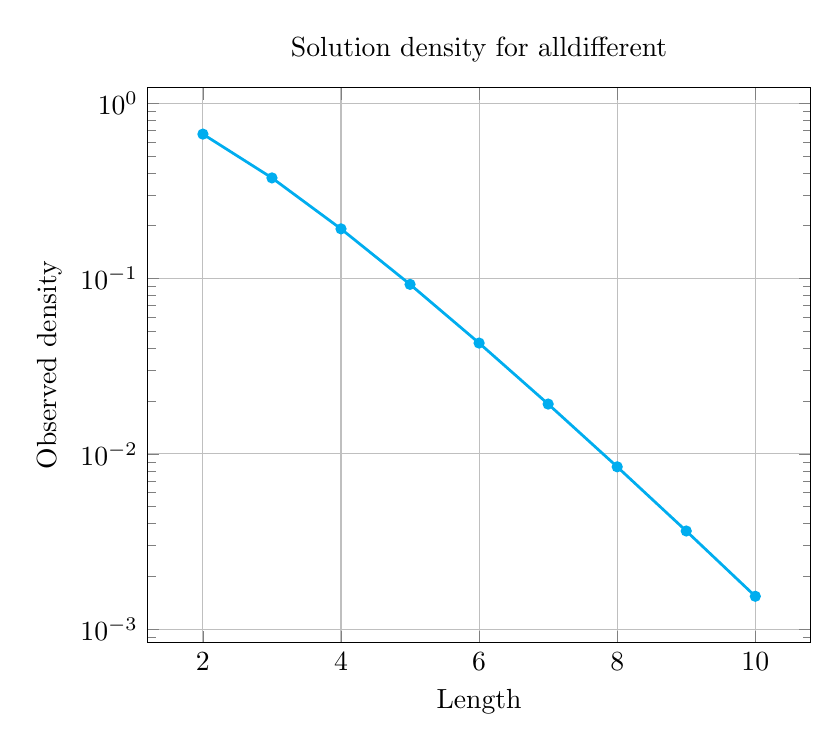
\begin{tikzpicture}
\begin{semilogyaxis}[title=Solution density for \ctrrefself{alldifferent},width=10cm,grid=major,xlabel=Length,ylabel=Observed density]
\addplot[cyan,mark=*,line width=1pt,mark size=1.5pt] coordinates{
(2, 0.6666666666666666)
(3, 0.375)
(4, 0.192)
(5, 0.09259259259259259)
(6, 0.042839293151662995)
(7, 0.01922607421875)
(8, 0.008429910375751965)
(9, 0.0036288)
(10, 0.0015389654375500732)
};
\end{semilogyaxis}
\end{tikzpicture}

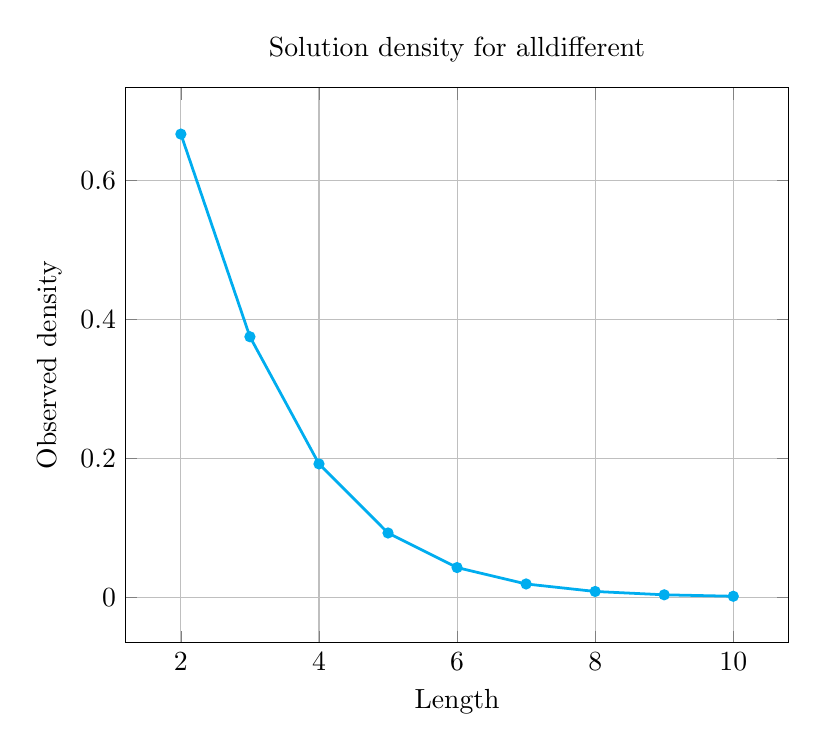
\begin{tikzpicture}
\begin{axis}[title=Solution density for \ctrrefself{alldifferent},width=10cm,grid=major,xlabel=Length,ylabel=Observed density]
\addplot[cyan,mark=*,line width=1pt,mark size=1.5pt] coordinates{
(2, 0.6666666666666666)
(3, 0.375)
(4, 0.192)
(5, 0.09259259259259259)
(6, 0.042839293151662995)
(7, 0.01922607421875)
(8, 0.008429910375751965)
(9, 0.0036288)
(10, 0.0015389654375500732)
};
\end{axis}
\end{tikzpicture}


\item[\pdfmarkup{subject={Systems},color=white,markup=Highlight}{Systems}{References to the constraint in some concrete constraint programming systems.}
]
\href{http://www.emn.fr/z-info/choco-solver/tex/documentation/choco-doc.pdf}{\texttt{allDifferent}} in \href{http://choco.emn.fr/}{{\bf Choco}},
\href{http://www.gecode.org/doc/3.7.0/reference/group__TaskModelIntDistinct.html}{\texttt{linear}} in \href{http://www.gecode.org/}{{\bf Gecode}},
\href{http://jacopapi.osolpro.com/JaCoP/constraints/Alldifferent.html}{\texttt{alldifferent}} in \href{http://www.jacop.eu/}{{\bf JaCoP}},
\href{http://jacopapi.osolpro.com/JaCoP/constraints/Alldiff.html}{\texttt{alldiff}} in \href{http://www.jacop.eu/}{{\bf JaCoP}},
\href{http://jacopapi.osolpro.com/JaCoP/constraints/Alldistinct.html}{\texttt{alldistinct}} in \href{http://www.jacop.eu/}{{\bf JaCoP}},
\href{http://www.g12.cs.mu.oz.au/minizinc/downloads/doc-1.4/mzn-globals.html#all_different}{\texttt{all\_different}} in \href{http://www.g12.cs.mu.oz.au/minizinc/}{{\bf MiniZinc}},
\href{http://www.sics.se/sicstus/docs/latest4/html/sicstus.html/Combinatorial-Constraints.html}{\texttt{all\_different}} in \href{http://www.sics.se/sicstus/}{{\bf SICStus}},
\href{http://www.sics.se/sicstus/docs/latest4/html/sicstus.html/Combinatorial-Constraints.html}{\texttt{all\_distinct}} in \href{http://www.sics.se/sicstus/}{{\bf SICStus}}.
\item[\pdfmarkup{subject={Used in},color=white,markup=Highlight}{Used in}{List of constraints that use this constraint in their description.}
\hypertarget{CalldifferentPlinks}{}
]
\hyperlink{Calldifferent_consecutive_values}{\ctrref{alldifferent\_consecutive\_values}},
\hyperlink{Ccircuit_cluster}{\ctrref{circuit\_cluster}},
\hyperlink{Ccorrespondence}{\ctrref{correspondence}},
\hyperlink{Ccumulative_convex}{\ctrref{cumulative\_convex}},
\hyperlink{Cmax_occ_of_consecutive_tuples_of_values}{\ctrref{max\_occ\_of\_consecutive\_tuples\_of\_values}},
\hyperlink{Cmax_occ_of_sorted_tuples_of_values}{\ctrref{max\_occ\_of\_sorted\_tuples\_of\_values}},
\hyperlink{Csize_max_seq_alldifferent}{\ctrref{size\_max\_seq\_alldifferent}},
\hyperlink{Csize_max_starting_seq_alldifferent}{\ctrref{size\_max\_starting\_seq\_alldifferent}},
\hyperlink{Csort_permutation}{\ctrref{sort\_permutation}}.
\item[\pdfmarkup{subject={See also},color=white,markup=Highlight}{See also}{Related constraints grouped by semantics links.}
]
\hyperlink{Lcommon_keyword}{{\bf common keyword:}}
\hyperlink{Ccircuit}{\ctrref{circuit}},
\hyperlink{Ccircuit_cluster}{\ctrref{circuit\_cluster}},
\hyperlink{Ccycle}{\ctrref{cycle}},
\hyperlink{Cderangement}{\ctrref{derangement}}\,\emph{(\hyperlink{permutation}{permutation}\index{permutation|indexuse})},
\hyperlink{Cgolomb}{\ctrref{golomb}}\,\emph{(\hyperlink{all_different}{all different}\index{all different|indexuse})},
\hyperlink{Cproper_circuit}{\ctrref{proper\_circuit}}\,\emph{(\hyperlink{permutation}{permutation}\index{permutation|indexuse})},
\hyperlink{Csize_max_seq_alldifferent}{\ctrref{size\_max\_seq\_alldifferent}},
\hyperlink{Csize_max_starting_seq_alldifferent}{\ctrref{size\_max\_starting\_seq\_alldifferent}}\,\emph{(\hyperlink{all_different}{all different}\index{all different|indexuse},\hyperlink{disequality}{disequality}\index{disequality|indexuse})},
\hyperlink{Csymmetric_alldifferent}{\ctrref{symmetric\_alldifferent}}\,\emph{(\hyperlink{permutation}{permutation}\index{permutation|indexuse})}.

\hyperlink{Lcost_variant}{{\bf cost variant:}}
\hyperlink{Cminimum_weight_alldifferent}{\ctrref{minimum\_weight\_alldifferent}},
\hyperlink{Cweighted_partial_alldiff}{\ctrref{weighted\_partial\_alldiff}}.

\hyperlink{Lgeneralisation}{{\bf generalisation:}}
\hyperlink{Call_min_dist}{\ctrref{all\_min\_dist}}\,\emph{($\argument{variable}$ replaced by $\argument{line~segment}$, all of the same size)},
\hyperlink{Calldifferent_between_sets}{\ctrref{alldifferent\_between\_sets}}\,\emph{($\argument{variable}$ replaced by $\argument{set~variable}$)},
\hyperlink{Calldifferent_cst}{\ctrref{alldifferent\_cst}}\,\emph{($\argument{variable}$ replaced by $\argument{variable}+\argument{constant}$)},
\hyperlink{Calldifferent_interval}{\ctrref{alldifferent\_interval}}\,\emph{($\argument{variable}$ replaced by $\argument{variable}/\argument{constant}$)},
\hyperlink{Calldifferent_modulo}{\ctrref{alldifferent\_modulo}}\,\emph{($\argument{variable}$ replaced by $\argument{variable}\mod \argument{constant}$)},
\hyperlink{Calldifferent_partition}{\ctrref{alldifferent\_partition}}\,\emph{($\argument{variable}$ replaced by $\argument{variable}\in \argument{partition}$)},
\hyperlink{Cdiffn}{\ctrref{diffn}}\,\emph{($\argument{variable}$ replaced by \hyperlink{orthotope}{orthotope}\index{orthotope|indexuse})},
\hyperlink{Cdisjunctive}{\ctrref{disjunctive}}\,\emph{($\argument{variable}$ replaced by $\argument{task}$)},
\hyperlink{Cglobal_cardinality}{\ctrref{global\_cardinality}}\,\emph{(control the number of occurrence of each value with a counter variable)},
\hyperlink{Cglobal_cardinality_low_up}{\ctrref{global\_cardinality\_low\_up}}\,\emph{(control the number of occurrence of each value with an interval)},
\hyperlink{Clex_alldifferent}{\ctrref{lex\_alldifferent}}\,\emph{($\argument{variable}$ replaced by $\argument{vector}$)},
\hyperlink{Cnvalue}{\ctrref{nvalue}}\,\emph{(count number of distinct values)}.

\hyperlink{Limplied_by}{{\bf implied by:}}
\hyperlink{Calldifferent_consecutive_values}{\ctrref{alldifferent\_consecutive\_values}},
\hyperlink{Ccircuit}{\ctrref{circuit}},
\hyperlink{Ccycle}{\ctrref{cycle}},
\hyperlink{Cstrictly_decreasing}{\ctrref{strictly\_decreasing}},
\hyperlink{Cstrictly_increasing}{\ctrref{strictly\_increasing}}.

\hyperlink{Limplies}{{\bf implies:}}
\hyperlink{Calldifferent_except_0}{\ctrref{alldifferent\_except\_0}},
\hyperlink{Cmulti_global_contiguity}{\ctrref{multi\_global\_contiguity}},
\hyperlink{Cnot_all_equal}{\ctrref{not\_all\_equal}}.

\hyperlink{Lnegation}{{\bf negation:}}
\hyperlink{Csome_equal}{\ctrref{some\_equal}}.

\hyperlink{Lpart_of_system_of_constraints}{{\bf part of system of constraints:}}
\hyperlink{Cneq}{\ctrref{neq}}.

\hyperlink{Lshift_of_concept}{{\bf shift of concept:}}
\hyperlink{Calldifferent_on_intersection}{\ctrref{alldifferent\_on\_intersection}},
\hyperlink{Calldifferent_same_value}{\ctrref{alldifferent\_same\_value}}.

\hyperlink{Lsoft_variant}{{\bf soft variant:}}
\hyperlink{Calldifferent_except_0}{\ctrref{alldifferent\_except\_0}}\,\emph{(value $0$ can be used several times)},
\hyperlink{Copen_alldifferent}{\ctrref{open\_alldifferent}}\,\emph{(\hyperlink{open_constraint}{open constraint}\index{open constraint|indexuse})},
\hyperlink{Csoft_alldifferent_ctr}{\ctrref{soft\_alldifferent\_ctr}}\,\emph{(\hyperlink{decomposition-based_violation_measure}{decomposition-based violation measure}\index{decomposition-based violation measure|indexuse})},
\hyperlink{Csoft_alldifferent_var}{\ctrref{soft\_alldifferent\_var}}\,\emph{(\hyperlink{variable-based_violation_measure}{variable-based violation measure}\index{variable-based violation measure|indexuse})}.

\hyperlink{Lsystem_of_constraints}{{\bf system of constraints:}}
\hyperlink{Ck_alldifferent}{\ctrref{k\_alldifferent}}.

\hyperlink{Lused_in_reformulation}{{\bf used in reformulation:}}
\hyperlink{Cin_interval_reified}{\ctrref{in\_interval\_reified}}\,\emph{(\hyperlink{bound-consistency}{bound-consistency}\index{bound-consistency|indexuse} preserving reformulation)},
\hyperlink{Csort}{\ctrref{sort}},
\hyperlink{Cstrictly_increasing}{\ctrref{strictly\_increasing}}.

\hyperlink{Luses_in_its_reformulation}{{\bf uses in its reformulation:}}
\hyperlink{Ccycle}{\ctrref{cycle}},
\hyperlink{Celements_alldifferent}{\ctrref{elements\_alldifferent}},
\hyperlink{Csort_permutation}{\ctrref{sort\_permutation}}.

\item[\pdfmarkup{subject={Keywords},color=white,markup=Highlight}{Keywords}{Related keywords grouped by meta-keywords.}
]
\hyperlink{characteristic_of_a_constraint}{{\bf characteristic of a constraint:}}\index{characteristic of a constraint|indexuse}
\hyperlink{core}{core},\index{core|indexuse}
\hyperlink{all_different}{all different},\index{all different|indexuse}
\hyperlink{disequality}{disequality},\index{disequality|indexuse}
\hyperlink{sort_based_reformulation}{sort based reformulation},\index{sort based reformulation|indexuse}
\hyperlink{automaton}{automaton},\index{automaton|indexuse}
\hyperlink{automaton_with_array_of_counters}{automaton with array of counters}.\index{automaton with array of counters|indexuse}
 
\hyperlink{combinatorial_object}{{\bf combinatorial object:}}\index{combinatorial object|indexuse}
\hyperlink{permutation}{permutation}.\index{permutation|indexuse}
 
\hyperlink{constraint_type}{{\bf constraint type:}}\index{constraint type|indexuse}
\hyperlink{system_of_constraints}{system of constraints},\index{system of constraints|indexuse}
\hyperlink{value_constraint}{value constraint}.\index{value constraint|indexuse}
 
\hyperlink{filtering}{{\bf filtering:}}\index{filtering|indexuse}
\hyperlink{bipartite_matching}{bipartite matching},\index{bipartite matching|indexuse}
\hyperlink{bipartite_matching_in_convex_bipartite_graphs}{bipartite matching in convex bipartite graphs},\index{bipartite matching in convex bipartite graphs|indexuse}
\hyperlink{convex_bipartite_graph}{convex bipartite graph},\index{convex bipartite graph|indexuse}
\hyperlink{flow}{flow},\index{flow|indexuse}
\hyperlink{Hall_interval}{Hall interval},\index{Hall interval|indexuse}
\hyperlink{arc-consistency}{arc-consistency},\index{arc-consistency|indexuse}
\hyperlink{bound-consistency}{bound-consistency},\index{bound-consistency|indexuse}
\hyperlink{SAT}{SAT},\index{SAT|indexuse}
\hyperlink{DFS-bottleneck}{DFS-bottleneck},\index{DFS-bottleneck|indexuse}
\hyperlink{entailment}{entailment}.\index{entailment|indexuse}
 
\hyperlink{final_graph_structure}{{\bf final graph structure:}}\index{final graph structure|indexuse}
\hyperlink{one_succ}{one\_succ}.\index{one\_succ|indexuse}
 
\hyperlink{modelling_exercises}{{\bf modelling exercises:}}\index{modelling exercises|indexuse}
\hyperlink{n-Amazons}{n-Amazons},\index{n-Amazons|indexuse}
\hyperlink{zebra_puzzle}{zebra puzzle}.\index{zebra puzzle|indexuse}
 
\hyperlink{problems}{{\bf problems:}}\index{problems|indexuse}
\hyperlink{maximum_clique}{maximum clique},\index{maximum clique|indexuse}
\hyperlink{graph_colouring}{graph colouring}.\index{graph colouring|indexuse}
 
\hyperlink{puzzles}{{\bf puzzles:}}\index{puzzles|indexuse}
\hyperlink{n-Amazons}{n-Amazons},\index{n-Amazons|indexuse}
\hyperlink{n-queens}{n-queens},\index{n-queens|indexuse}
\hyperlink{Costas_arrays}{Costas arrays},\index{Costas arrays|indexuse}
\hyperlink{Euler_knight}{Euler knight},\index{Euler knight|indexuse}
\hyperlink{Golomb_ruler}{Golomb ruler},\index{Golomb ruler|indexuse}
\hyperlink{magic_hexagon}{magic hexagon},\index{magic hexagon|indexuse}
\hyperlink{magic_square}{magic square},\index{magic square|indexuse}
\hyperlink{zebra_puzzle}{zebra puzzle},\index{zebra puzzle|indexuse}
\hyperlink{Sudoku}{Sudoku}.\index{Sudoku|indexuse}
 
\item[\pdfmarkup{subject={Cond. implications},color=white,markup=Highlight}{Cond. implications}{Conditional implications.}]
\vspace{0.1pt}
\begin{minipage}[t]{11.2cm}
$\bullet$ $\constraint{alldifferent}(\argument{VARIABLES})$\\
\hspace*{7pt}{\bf implies}\hspace*{1pt} $ $\hyperlink{Clex_alldifferent}{\ctrref{lex\_alldifferent}}$(\argument{VECTORS}:\argument{VARIABLES})$.
\end{minipage}
\vspace{0.16cm}

 \begin{minipage}[t]{11.2cm}
$\bullet$ $\constraint{alldifferent}(\argument{VARIABLES})$\\
\hspace*{7pt}{\bf implies}\hspace*{1pt} $ $\hyperlink{Csoft_alldifferent_ctr}{\ctrref{soft\_alldifferent\_ctr}}$(\argument{C},\argument{VARIABLES})$.
\end{minipage}
\vspace{0.16cm}

 \begin{minipage}[t]{11.2cm}
$\bullet$ $\constraint{alldifferent}(\argument{VARIABLES})$\\
\hspace*{7pt}{\bf implies}\hspace*{1pt} $ $\hyperlink{Cbalance}{\ctrref{balance}}$(\argument{BALANCE},\argument{VARIABLES})$\\
 \hspace*{10pt} when\hspace*{3pt} $\argument{BALANCE}=0$.
\end{minipage}
\vspace{0.16cm}

 \begin{minipage}[t]{11.2cm}
$\bullet$ $\constraint{alldifferent}(\argument{VARIABLES})$\\
\hspace*{7pt}{\bf implies}\hspace*{1pt} $ $\hyperlink{Csoft_all_equal_max_var}{\ctrref{soft\_all\_equal\_max\_var}}$(\argument{N},\argument{VARIABLES})$\\
 \hspace*{10pt} when\hspace*{3pt} $\argument{N}<|\argument{VARIABLES}|$.
\end{minipage}
\vspace{0.16cm}

 \begin{minipage}[t]{11.2cm}
$\bullet$ $\constraint{alldifferent}(\argument{VARIABLES})$\\
\hspace*{7pt}{\bf implies}\hspace*{1pt} $ $\hyperlink{Csoft_all_equal_min_var}{\ctrref{soft\_all\_equal\_min\_var}}$(\argument{N},\argument{VARIABLES})$\\
 \hspace*{10pt} when\hspace*{3pt} $\argument{N}>|\argument{VARIABLES}|$.
\end{minipage}
\vspace{0.16cm}

 \begin{minipage}[t]{11.2cm}
$\bullet$ $\constraint{alldifferent}(\argument{VARIABLES})$\\
\hspace*{7pt}{\bf implies}\hspace*{1pt} $ $\hyperlink{Cchange}{\ctrref{change}}$(\argument{NCHANGE},\argument{VARIABLES},\argument{CTR})$\\
 \hspace*{10pt} when\hspace*{3pt} $\argument{NCHANGE}=|\argument{VARIABLES}|-1$\\
 \hspace*{10pt} and\hspace*{9pt} $\argument{CTR}\in \lb\neq \rb$.
\end{minipage}
\vspace{0.16cm}

 \begin{minipage}[t]{11.2cm}
$\bullet$ $\constraint{alldifferent}(\argument{VARIABLES})$\\
\hspace*{7pt}{\bf implies}\hspace*{1pt} $ $\hyperlink{Ccircular_change}{\ctrref{circular\_change}}$(\argument{NCHANGE},\argument{VARIABLES},\argument{CTR})$\\
 \hspace*{10pt} when\hspace*{3pt} $\argument{NCHANGE}=|\argument{VARIABLES}|$\\
 \hspace*{10pt} and\hspace*{9pt} $\argument{CTR}\in \lb\neq \rb$.
\end{minipage}
\vspace{0.16cm}

 \begin{minipage}[t]{11.2cm}
$\bullet$ $\constraint{alldifferent}(\argument{VARIABLES})$\\
\hspace*{7pt}{\bf implies}\hspace*{1pt} $ $\hyperlink{Clongest_change}{\ctrref{longest\_change}}$(\argument{SIZE},\argument{VARIABLES},\argument{CTR})$\\
 \hspace*{10pt} when\hspace*{3pt} $\argument{SIZE}=|\argument{VARIABLES}|$\\
 \hspace*{10pt} and\hspace*{9pt} $\argument{CTR}\in \lb\neq \rb$.
\end{minipage}
\vspace{0.16cm}

 \begin{minipage}[t]{11.2cm}
$\bullet$ $\constraint{alldifferent}(\argument{VARIABLES})$\\
 \hspace*{10pt} with\hspace*{3pt} $|\argument{VARIABLES}|>0$\\
\hspace*{7pt}{\bf implies}\hspace*{1pt} $ $\hyperlink{Clength_first_sequence}{\ctrref{length\_first\_sequence}}$(\argument{LEN},\argument{VARIABLES})$\\
 \hspace*{10pt} when\hspace*{3pt} $\argument{LEN}=1$.
\end{minipage}
\vspace{0.16cm}

 \begin{minipage}[t]{11.2cm}
$\bullet$ $\constraint{alldifferent}(\argument{VARIABLES})$\\
 \hspace*{10pt} with\hspace*{3pt} $|\argument{VARIABLES}|>0$\\
\hspace*{7pt}{\bf implies}\hspace*{1pt} $ $\hyperlink{Clength_last_sequence}{\ctrref{length\_last\_sequence}}$(\argument{LEN},\argument{VARIABLES})$\\
 \hspace*{10pt} when\hspace*{3pt} $\argument{LEN}=1$.
\end{minipage}
\vspace{0.16cm}

 \begin{minipage}[t]{11.2cm}
$\bullet$ $\constraint{alldifferent}(\argument{VARIABLES})$\\
 \hspace*{10pt} with\hspace*{3pt} $|\argument{VARIABLES}|>0$\\
\hspace*{7pt}{\bf implies}\hspace*{1pt} $ $\hyperlink{Cmin_nvalue}{\ctrref{min\_nvalue}}$(\argument{MIN},\argument{VARIABLES})$\\
 \hspace*{10pt} when\hspace*{3pt} $\argument{MIN}=1$.
\end{minipage}
\vspace{0.16cm}

 \clearpage
\colorbox{MyAzurelight}{\begin{minipage}[t]{11.2cm}
\colorbox{MyAzurelight}{\begin{minipage}[t]{11.2cm}
\item[Arc input(s)]
\hypertarget{CalldifferentPgraph}{}
$\argument{VARIABLES}$
\item[Arc generator]
\begin{tabular}[t]{l}
$ $\hyperlink{AG_CLIQUE}{$\arcgenerator{CLIQUE}$}$ \mapsto  $\hyperlink{DT_collection}{$\argument{collection}$}$ (\argument{variables1},\argument{variables2})$\\
\end{tabular}
\index{CLIQUE@$\arcgenerator{CLIQUE}$|indexuse}
\item[Arc arity]
\begin{tabular}[t]{l}
$2$\\
\end{tabular}
\item[Arc constraint(s)]
\begin{tabular}[t]{l}
$\argument{variables1}.\argument{var}=\argument{variables2}.\argument{var}$\\
\end{tabular}
\item[Graph property(ies)]
\begin{tabular}[t]{l}
$ $\hyperlink{GC_MAX_NSCC}{$\graphproperty{MAX\_NSCC}$}$ \leq 1$\\
\end{tabular}
\index{MAX\_NSCC@$\graphproperty{MAX\_NSCC}$|indexuse}
\item[Graph class]
\begin{tabular}[t]{l}
$ $\hyperlink{GC_ONE_SUCC}{$\graphclass{ONE\_SUCC}$}$ $\\
\end{tabular}
\index{ONE\_SUCC@$\graphclass{ONE\_SUCC}$|indexuse}
\hrule

\end{minipage}}

\end{minipage}}
\item[\pdfmarkup{subject={Graph model},color=white,markup=Highlight}{Graph model}{Explicit description in terms of graph property of the meaning of the constraint.}]
We generate a \emph{clique} with an \emph{equality} constraint
between each pair of vertices (including a vertex and itself) and
state that the size of the largest strongly connected component should
not exceed one.

Parts~(A) and~(B) of Figure~\ref{fig:alldifferent} respectively show the initial and final graph
associated with the {\bf Example} slot.
Since we use the \hyperlink{GC_MAX_NSCC}{$\MMAXNSCC$} graph property we show one
of the largest strongly connected component of the final graph.
The \ctrrefself{alldifferent} holds since all the strongly connected
components have at most one vertex: a value is used at most once.

\examplefig

\clearpage
\item[\pdfmarkup{subject={Automaton},color=white,markup=Highlight}{Automaton}{Explicit description in terms of automaton of the meaning of the constraint.}]
\hypertarget{CalldifferentPauto}{}
Figure~\ref{fig:alldifferent1} depicts the \hyperlink{automaton}{automaton}
associated with the \ctrrefself{alldifferent} constraint.
To each item of the collection $\argument{VARIABLES}$
corresponds a signature variable $\argument{S}_i$ that is equal to $1$.
The \hyperlink{automaton}{automaton} counts the number of occurrences of each
value and finally imposes that each value is taken at most one time.

\begin{figure}[!h]
\centering
{\footnotesize
\newcommand{\Carrayfigalldifferent}{$\{C[\_]\leftarrow 0\}$}
\begin{tikzpicture}[->,>=stealth',shorten >=1pt,auto,node distance=18mm,semithick]
\node[rectangle,draw,fill=green!10] at (0,-1.2) (ctr) {\hyperlink{Carith}{\ctrref{arith}}$(C,<,2)$};
\node[initial,accepting,initial text=\Carrayfigalldifferent,initial distance=10mm,state,fill=MyYellowlight] (s) {$s$};
\path
(s) edge [loop right]  node {$\begin{array}{l} 1, \\ \{C[\argument{VAR}_i]\leftarrow C[\argument{VAR}_i]+1\}\end{array}$}	 (s);
\draw  [dotted,-] (s) -- (ctr);
\end{tikzpicture}
\caption{\label{fig:alldifferent1}
Automaton of the \ctrrefself{alldifferent} constraint}
}
\end{figure}

\item[\pdfmarkup{subject={Quiz},color=white,markup=Highlight}{Quiz}{A set of small exercises for checking that the meaning of the constraint is well understood.}]
\hspace*{0.4em}~\label{exercises_alldifferent}

% Hint:
% go back to the definition of alldifferent.
{\small
\exercisecaption{\ctrrefself{alldifferent}: checking whether a ground instance holds or not}
\renewcommand\theenumi {\bf\Alph{enumi}}
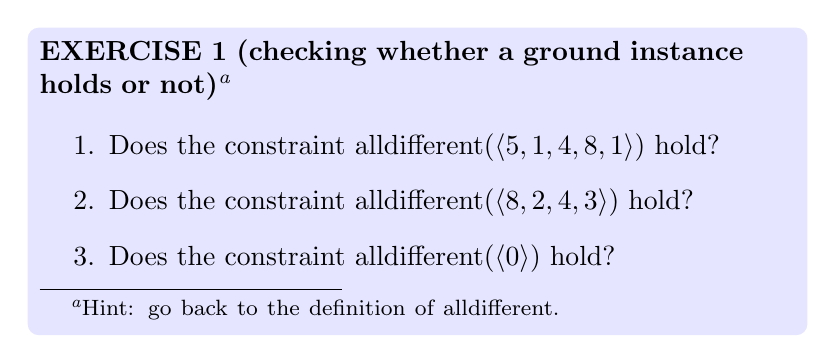
\begin{tikzpicture}
[information text/.style={rounded corners,inner sep=1ex}]
\draw
node[right,text width=9.6cm,information text,fill=blue!10]
{{\bf EXERCISE 1 (checking whether a ground instance holds or not)\footnote{Hint:
go back to the definition of \ctrrefself{alldifferent}.}}\\
\begin{enumerate}
\item Does the constraint \ctrrefself{alldifferent}$(\langle 5,1,4,8,1\rangle)$ hold?\\
\item Does the constraint \ctrrefself{alldifferent}$(\langle 8,2,4,3\rangle)$ hold?\\
\item Does the constraint \ctrrefself{alldifferent}$(\langle 0\rangle)$ hold?
\end{enumerate}
};
\end{tikzpicture}
}
~\\

% Hint:
% identify infeasible values,
% enumerate solutions in lexicographic order.
{\small
\exercisecaption{\ctrrefself{alldifferent}: finding all solutions}
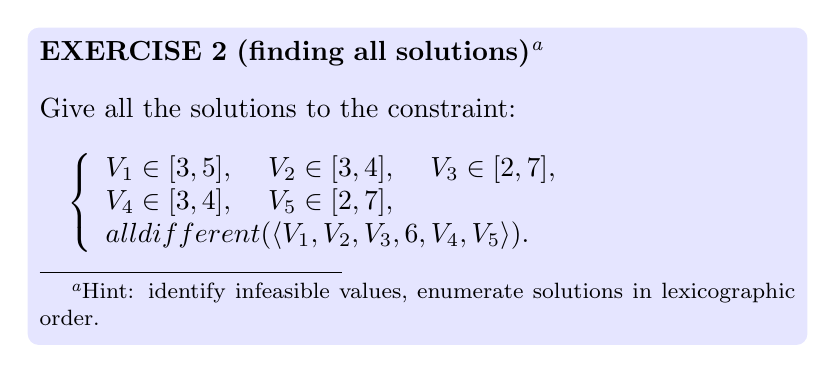
\begin{tikzpicture}
[information text/.style={rounded corners,inner sep=1ex}]
\draw
node[right,text width=9.6cm,information text,fill=blue!10]
{{\bf EXERCISE 2 (finding all solutions)\footnote{Hint: identify infeasible values,
enumerate solutions in lexicographic order.}}\\
\vspace{0.3cm}
Give all the solutions to the constraint:\\~\\
\hspace*{1em}$\left\{
\begin{array}{l l l}
V_1\in[3,5], ~& V_2\in[3,4], ~& V_3\in[2,7], \\
V_4\in[3,4], ~& V_5\in[2,7], \\
\multicolumn{3}{l}{\constraint{alldifferent}(\langle V_1,V_2,V_3,6,V_4,V_5\rangle).}
\end{array}
\right.$\\~\\
};
\end{tikzpicture}
}
~\\

% Hint:
% focus on variables with smallest domain first,
% identify Hall intervals for finding infeasible values,
% enumerate solutions in lexicographic order.
{\small
\exercisecaption{\ctrrefself{alldifferent}: finding all solutions}
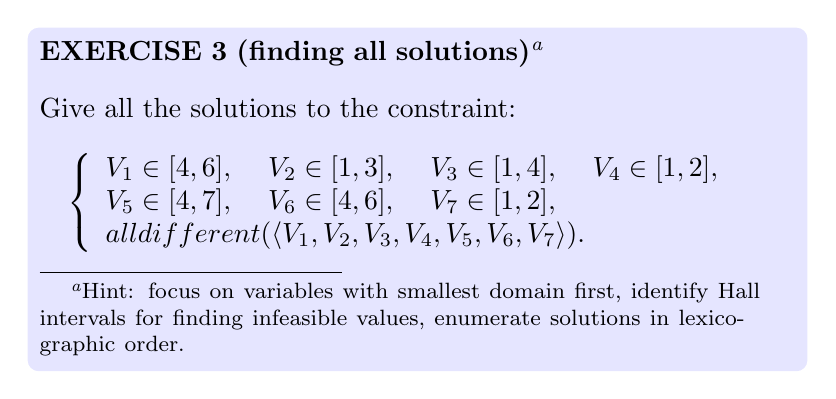
\begin{tikzpicture}
[information text/.style={rounded corners,inner sep=1ex}]
\draw
node[right,text width=9.6cm,information text,fill=blue!10]
{{\bf EXERCISE 3 (finding all solutions)\footnote{Hint: focus on variables with smallest domain first,
identify Hall intervals for finding infeasible values, enumerate solutions in lexicographic order.}}\\
\vspace{0.3cm}
Give all the solutions to the constraint:\\~\\
\hspace*{1em}$\left\{
\begin{array}{l l l l}
V_1\in[4,6],  ~& V_2\in[1,3], ~& V_3\in[1,4], ~& V_4\in[1,2], \\
V_5\in[4,7], ~& V_6\in[4,6], ~& V_7\in[1,2], \\
\multicolumn{4}{l}{\constraint{alldifferent}(\langle V_1,V_2,V_3,V_4,V_5,V_6,V_7\rangle).}
\end{array}
\right.$\\~\\
};
\end{tikzpicture}
}
~\\

% Hint:
% focus on variables with smallest domain first,
% identify Hall sets for finding infeasible values,
% enumerate solutions in lexicographic order.
{\small
\exercisecaption{\ctrrefself{alldifferent}: finding all solutions}
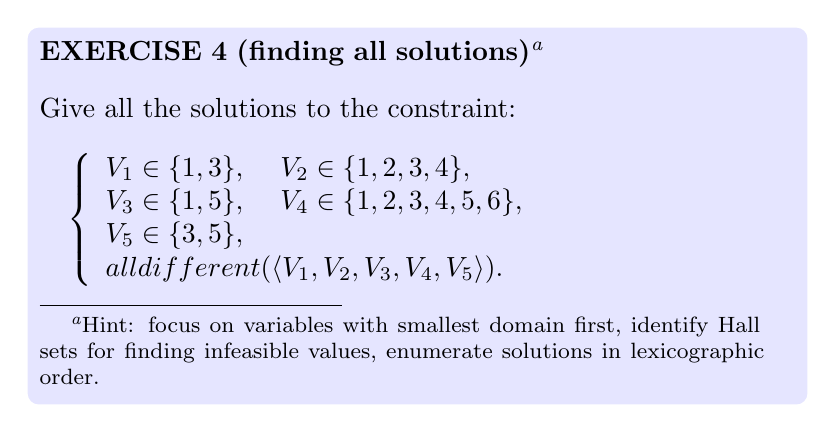
\begin{tikzpicture}
[information text/.style={rounded corners,inner sep=1ex}]
\draw
node[right,text width=9.6cm,information text,fill=blue!10]
{{\bf EXERCISE 4 (finding all solutions)\footnote{Hint: focus on variables with smallest domain first,
identify Hall sets for finding infeasible values,
enumerate solutions in lexicographic order.}}\\
\vspace{0.3cm}
Give all the solutions to the constraint:\\~\\
\hspace*{1em}$\left\{
\begin{array}{l l}
V_1\in\{1,3\}, ~& V_2\in\{1,2,3,4\}, \\
V_3\in\{1,5\}, ~& V_4\in\{1,2,3,4,5,6\}, \\
V_5\in\{3,5\}, \\
\multicolumn{2}{l}{\constraint{alldifferent}(\langle V_1,V_2,V_3,V_4,V_5\rangle).}
\end{array}
\right.$\\~\\
};
\end{tikzpicture}
}
~\\

% Hint:
% focus on variables with smallest domain first,
% identify Hall sets for finding infeasible values.
{\small
\exercisecaption{\ctrrefself{alldifferent}: identifying infeasible values}
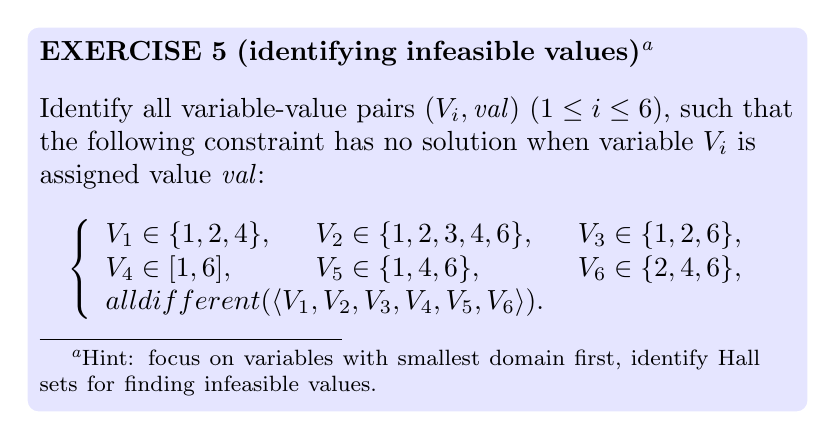
\begin{tikzpicture}
[information text/.style={rounded corners,inner sep=1ex}]
\draw
node[right,text width=9.6cm,information text,fill=blue!10]
{{\bf EXERCISE 5 (identifying infeasible values)\footnote{Hint: focus on variables with smallest domain first,
identify Hall sets for finding infeasible values.}}\\
\vspace{0.3cm}
Identify all variable-value pairs $(V_i,\mathit{val})$ $(1\leq i\leq 6)$, such that the following constraint
has no solution when variable $V_i$ is assigned value $\mathit{val}$:\\~\\
\hspace*{1em}$\left\{
\begin{array}{l l l}
V_1\in\{1,2,4\},		~~& V_2\in\{1,2,3,4,6\},	~~& V_3\in\{1,2,6\}, \\
V_4\in[1,6],		~~& V_5\in\{1,4,6\},		~~& V_6\in\{2,4,6\}, \\
\multicolumn{3}{l}{\constraint{alldifferent}(\langle V_1,V_2,V_3,V_4,V_5,V_6\rangle).}
\end{array}
\right.$\\~\\
};
\end{tikzpicture}
}
~\\

% Hint:
% group together variables that belong to the same set of constraints
% and reason on the number of distinct values assigned to such groups.
{\small
\exercisecaption{\ctrrefself{alldifferent}: identifying infeasible values and counting}
\renewcommand\theenumi {\bf\Alph{enumi}}
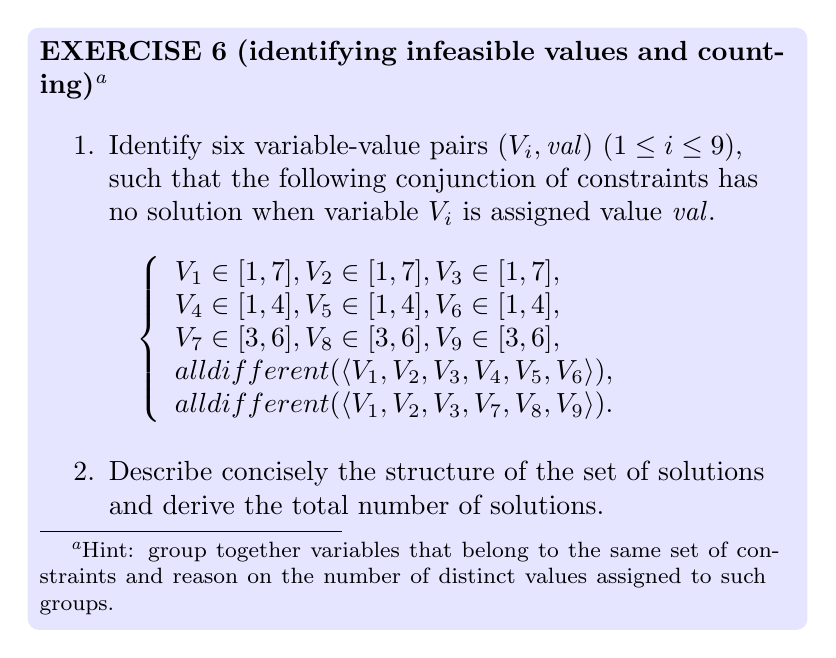
\begin{tikzpicture}
[information text/.style={rounded corners,inner sep=1ex}]
\draw node[right,text width=9.6cm,information text,fill=blue!10]
{{\bf EXERCISE 6 (identifying infeasible values and counting)\footnote{Hint: group together variables that belong to the same set of constraints and reason on the number of distinct values assigned to such groups.}}\\
\begin{enumerate}
\item
Identify six variable-value pairs $(V_i,\mathit{val})$ $(1\leq i\leq 9)$, such that the following
conjunction of constraints has no solution when variable $V_i$ is assigned value $\mathit{val}$.\\~\\
\hspace*{1em}$\left\{
\begin{array}{l}
V_1\in [1,7], V_2\in [1,7], V_3\in [1,7],\\
V_4\in [1,4], V_5\in [1,4], V_6\in [1,4],\\
V_7\in [3,6], V_8\in [3,6], V_9\in [3,6],\\
\constraint{alldifferent}(\langle V_1,V_2,V_3,V_4,V_5,V_6\rangle),\\
\constraint{alldifferent}(\langle V_1,V_2,V_3,V_7,V_8,V_9\rangle).\\
\end{array}
\right.$\\~\\
\item
Describe concisely the structure of the set of solutions and derive the total number of solutions.
\end{enumerate}
};
\end{tikzpicture}
}
~\\

% Hint:
% focus on the groups of variables that are assigned the same value.
{\small
\exercisecaption{\ctrrefself{alldifferent}: variable-based degree of violation}
\renewcommand\theenumi {\bf\Alph{enumi}}
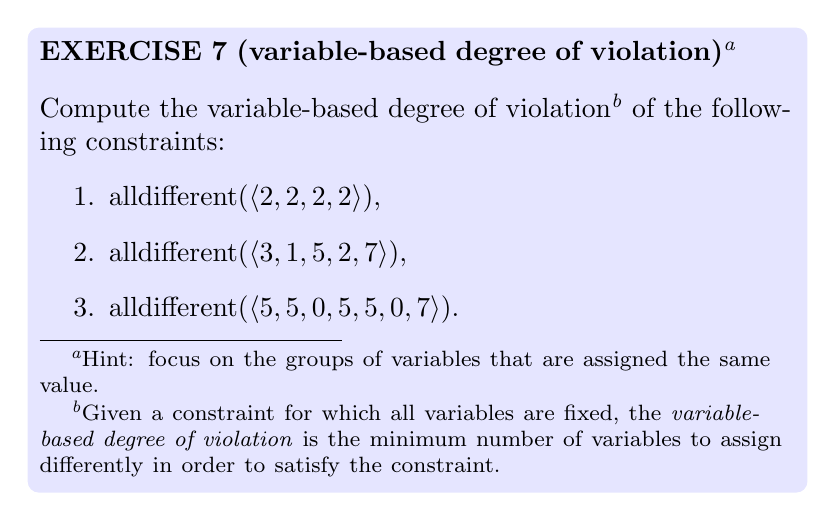
\begin{tikzpicture}
[information text/.style={rounded corners,inner sep=1ex}]
\draw
node[right,text width=9.6cm,information text,fill=blue!10]
{{\bf EXERCISE 7 (variable-based degree of violation)\footnote{Hint: focus on the groups of variables that are assigned the same value.}}\\
\vspace{0.3cm}
Compute the variable-based degree of violation\footnote{Given a constraint for which
all variables are fixed, the \emph{variable-based degree of violation} is the minimum number
of variables to assign differently in order to satisfy the constraint.} of the following constraints:
\begin{enumerate}
\item  \ctrrefself{alldifferent}$(\langle 2, 2, 2, 2\rangle)$,
\item  \ctrrefself{alldifferent}$(\langle 3, 1, 5, 2, 7\rangle)$,
\item  \ctrrefself{alldifferent}$(\langle 5, 5, 0, 5, 5, 0, 7\rangle)$.
\end{enumerate}
};
\end{tikzpicture}
}
~\\

% Hint:
% break some symmetry of the problem.
{\small
\exercisecaption{\ctrrefself{alldifferent}: preventing conflict around the table}
\renewcommand\theenumi{\protect\setcounter{local}%
{171+\the\value{enumi}}\protect{\ding{\value{local}}}}
\renewcommand\labelenumi{\theenumi}
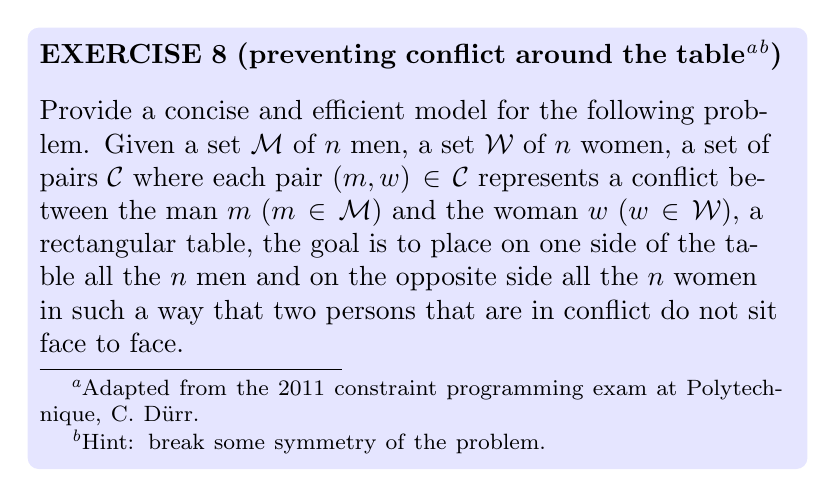
\begin{tikzpicture}
[information text/.style={rounded corners,inner sep=1ex}]
\draw[xshift=0cm,yshift=0cm]
node[right,text width=9.6cm,information text,fill=blue!10]
{{\bf EXERCISE 8 (preventing conflict around the table}\footnote{Adapted
from the 2011 constraint programming exam at Polytechnique, C.~D\"{u}rr.}\footnote{Hint:
break some symmetry of the problem.}{\bf)}\\
\vspace{0.3cm}
Provide a concise and efficient model for the following problem.
Given a set $\mathcal{M}$ of $n$ men,
a set $\mathcal{W}$ of $n$ women,
a set of pairs $\mathcal{C}$ where each pair $(m,w)\in\mathcal{C}$
represents a conflict between the man $m$ $(m\in\mathcal{M})$ and the woman $w$ $(w\in\mathcal{W})$,
a rectangular table,
the goal is to place on one side of the table all the $n$ men and on the opposite side all the $n$ women
in such a way that two persons that are in conflict do not sit face to face.
};
\end{tikzpicture}
}
~\\

% Hint:
% restrict extra values wrt a clique of disequalities.
{\small
\exercisecaption{\ctrrefself{alldifferent}: identifying equalities from a clique of disequalities}
\renewcommand\theenumi {\bf\Alph{enumi}}
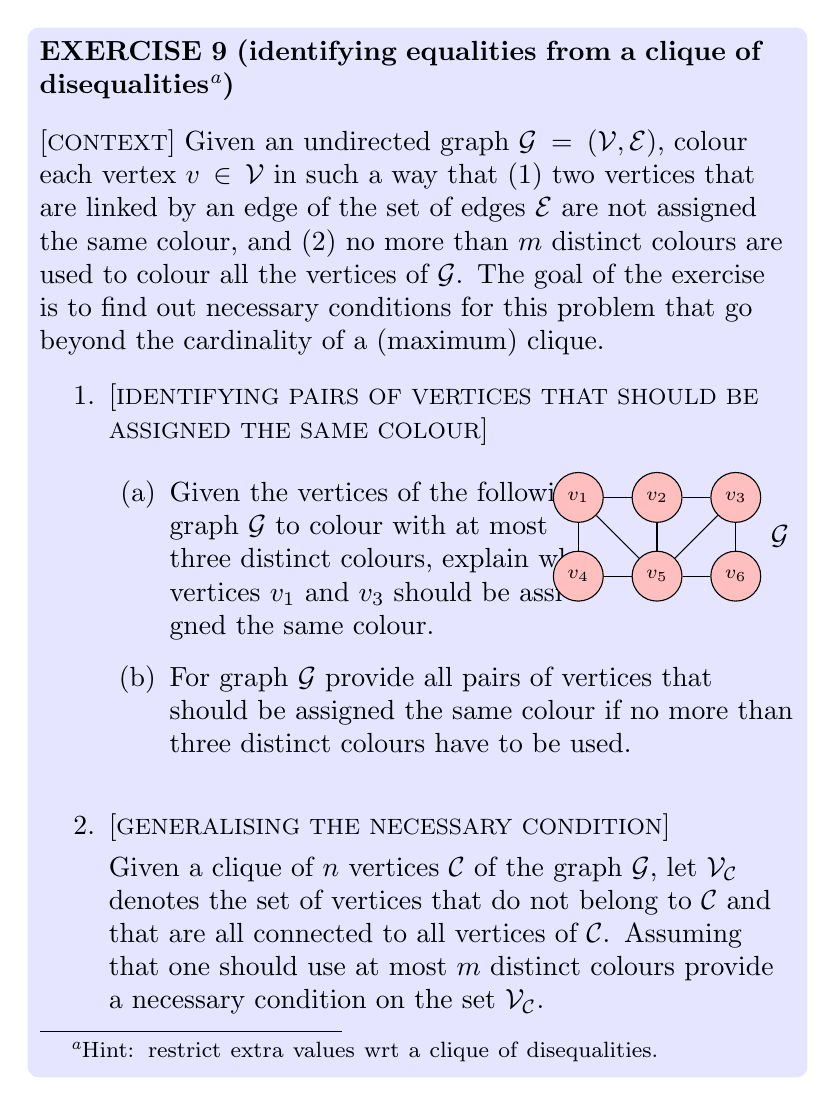
\begin{tikzpicture}
[information text/.style={rounded corners,inner sep=1ex}]
\draw[xshift=0cm,yshift=0cm]
node[right,text width=9.6cm,information text,fill=blue!10]
{{\bf EXERCISE 9 (identifying equalities from a clique of disequalities}\footnote{Hint:
restrict extra values wrt a clique of disequalities.}{\bf)}\\
\vspace{0.3cm}
$[${\footnotesize CONTEXT}$]$ Given an undirected graph $\mathcal{G}=(\mathcal{V},\mathcal{E})$, colour each vertex $v\in\mathcal{V}$
in such a way that
(1)~two vertices that are linked by an edge of the set of edges $\mathcal{E}$ are not assigned the same colour, and
(2)~no more than $m$ distinct colours are used to colour all the vertices of $\mathcal{G}$.
The goal of the exercise is to find out necessary conditions for this problem that go beyond
the cardinality of a (maximum) clique.
\begin{enumerate}
\item $[${\footnotesize IDENTIFYING PAIRS OF VERTICES THAT SHOULD BE ASSIGNED THE SAME COLOUR}$]$
\vspace{0.1cm}
\begin{enumerate}
\item Given the vertices of the following \\
graph $\mathcal{G}$ to colour with at most \\
three distinct colours, explain why \\
vertices $v_1$ and $v_3$ should be assi- \\
gned the same colour.
\vspace{0.1cm}
\item For graph $\mathcal{G}$ provide all pairs of vertices that should be assigned the same colour if no more than
three distinct colours have to be used.
\end{enumerate}
\vspace{0.2cm}
\item $[${\footnotesize GENERALISING THE NECESSARY CONDITION}$]$\\
\vspace{0.1cm}
Given a clique of $n$ vertices $\mathcal{C}$ of the graph $\mathcal{G}$,
let $\mathcal{V}_\mathcal{C}$ denotes the set of vertices that do not belong
to $\mathcal{C}$ and that are all connected to all vertices of $\mathcal{C}$.
Assuming that one should use at most $m$ distinct colours provide a necessary
condition on the set $\mathcal{V}_\mathcal{C}$.
\end{enumerate}
};
\begin{scope}[xshift=7cm,yshift=0.7cm,vertex/.style={circle,fill=pink,draw}]
\node[vertex] (1)			{\scriptsize$v_1$};
\node[vertex] (2) [right of=1]	{\scriptsize$v_2$};
\node[vertex] (3) [right of=2]	{\scriptsize$v_3$};
\node[vertex] (4) [below of=1]	{\scriptsize$v_4$};
\node[vertex] (5) [right of=4]	{\scriptsize$v_5$};
\node[vertex] (6) [right of=5]	{\scriptsize$v_6$};
\path
(1) 	edge 			node {} (2)
edge				node {} (4)
edge				node {} (5)
(2)	edge				node {} (3)
edge				node {} (5)
(3)	edge				node {} (5)
edge				node {} (6)
(4)	edge				node {} (5)
(5)	edge				node {} (6);
\coordinate [label=left:{$\mathcal{G}$}] (L) at (2.8,-0.5);
\end{scope}
\end{tikzpicture}
}
~\\

% Hint:
% consider each of the $4$ remaining positions on column c; extract information from the conjunction of the three \ctrrefself{alldifferent} constraints that allows the modelling of the $n$-queens problem.
{\small
\exercisecaption{\ctrrefself{alldifferent}: ($8$-queens) unfeasibility of a partial solution}
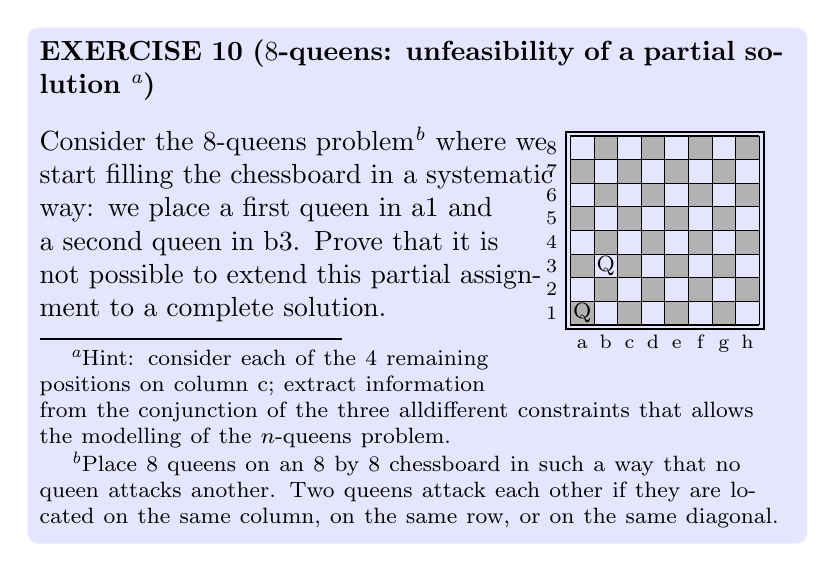
\begin{tikzpicture}
[information text/.style={rounded corners,inner sep=1ex}]
\draw[xshift=0cm,yshift=0cm]
node[right,text width=9.6cm,information text,fill=blue!10]
{{\bf EXERCISE 10 ($8$-queens: unfeasibility of a partial solution}
\footnote{Hint: consider each of the $4$ remaining \\
positions on column c; extract information \\
from the conjunction of the three \ctrrefself{alldifferent} constraints
that allows the modelling of the $n$-queens problem.}{\bf)}\\
\vspace{0.3cm}
Consider the $8$-queens problem\footnote{Place $8$ queens on an $8$ by $8$ chessboard in such a way that no queen attacks another. Two queens attack each other if they are located on the same column, on the same row, or on the same diagonal.} where we \\
start filling the chessboard in a systematic \\
way: we place a first queen in a$1$ and \\
a second queen in b$3$. Prove that it is \\
not possible to extend this partial assign- \\
ment to a complete solution.
};
\begin{scope}[xshift=6.9cm,yshift=-0.5cm,scale=0.3]
\draw[color=black,thick] (-0.18,-0.18) rectangle (8.18,8.18);
\foreach \x in {0,1,2,3} \foreach \y in {0,1,2,3} \fill [gray!60] (2*\x,2*\y) rectangle (2*\x+1,2*\y+1);
\foreach \x in {0,1,2,3} \foreach \y in {0,1,2,3} \fill [gray!60] (2*\x+1,2*\y+1) rectangle (2*\x+2,2*\y+2);
\draw (0.5,0.5) node{{\footnotesize\figsymbol{Q}}};
\draw (1.5,2.5) node{{\footnotesize\figsymbol{Q}}};
\foreach \x/\y in {1/a,2/b,3/c,4/d,5/e,6/f,7/g,8/h}
\node[anchor=base] at (\x-0.5,-1) {\scriptsize \y};
\foreach \x in {1,2,3,4,5,6,7,8}
\coordinate [label=left:{\scriptsize $\x$}] (X) at (-0.15,\x-0.5);
\draw (0,0) grid (8,8);
\end{scope}
\end{tikzpicture}
}
\ifweb\else
\newpage
\fi

{\small
\renewcommand\theenumi {\bf\Alph{enumi}}
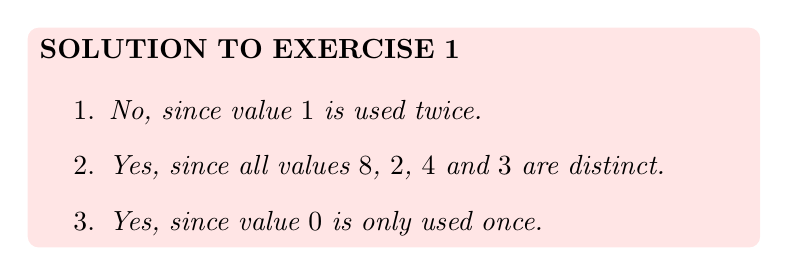
\begin{tikzpicture}
[information text/.style={rounded corners,inner sep=1ex}]
\draw[xshift=0cm,yshift=0cm]
node[right,text width=9.0cm,information text,fill=red!10]
{{\bf SOLUTION TO EXERCISE 1}\\
\begin{enumerate}
\item \emph{No, since value $1$ is used twice.}\\
\item \emph{Yes, since all values $8$, $2$, $4$ and $3$ are distinct.}\\
\item \emph{Yes, since value $0$ is only used once.}
\end{enumerate}
};
\end{tikzpicture}
}
~\\

{\small
\begin{tikzpicture}
[information text/.style={rounded corners,inner sep=1ex}]
\draw
node[right,text width=9.0cm,information text]
{{\bf SOLUTION TO EXERCISE 2}};
\begin{scope}[xshift=3cm,yshift=-1.9cm]
\node [single arrow, single arrow tip angle=135, single arrow head extend=1cm, draw=MyCornflowerBlue, line width=2pt,fill=MyYellowlight, single arrow, shape border rotate=270, text width=2.5cm, label=above:{{{\color{MyCornflowerBlue}\bf the four solutions}}}]
{{\tiny~~$\langle V_1,V_2,V_3,V_4,V_5\rangle$}\\
\ding{172} $(\langle 5,3,2,4,7\rangle)$\\
\ding{173} $(\langle 5,3,7,4,2\rangle)$\\
\ding{174} $(\langle 5,4,2,3,7\rangle)$\\
\ding{175} $(\langle 5,4,7,3,2\rangle)$};
\end{scope}
\draw[xshift=5.8cm,yshift=-2.1cm]
node[right,text width=2.8cm,information text,fill=red!10]
{
\emph{Values $3$ and $4$ have to be assigned to the two variables
$V_2$ and $V_4$.
Consequently, $V_1$, $V_3$ and $V_5$
are different from $3$ and $4$.}
};
\draw[xshift=0cm,yshift=-5.0cm]
node[right,text width=8.6cm,information text,fill=red!10]
{
\emph{Values $3$, $4$ and $5$ have to be assigned to
$V_1$, $V_2$ and $V_4$. Value $6$ is directly mentioned in the constraint.
Consequently the two remaining variables $V_3$ and $V_5$
can only be assigned values $2$ and $7$.
}
};
\end{tikzpicture}
}
~\\

{\small
\renewcommand\theenumi{\protect\setcounter{local}%
{181+\the\value{enumi}}\protect{\color{red!60}\ding{\value{local}}}}
\renewcommand\labelenumi{\theenumi}
\begin{tikzpicture}
[information text/.style={rounded corners,inner sep=1ex}]
\draw[xshift=0.0cm,yshift=0.0cm]
node[right,text width=9.6cm,information text]
{{\bf SOLUTION TO EXERCISE 3}};
\begin{scope}[xshift=2.5cm,yshift=-2.2cm]
\matrix (magic) [matrix of nodes] {
~   &     ~      &    ~      &     ~      &     ~                                 &     ~     &{\bf 7} &    ~      \\
~   &     ~      &    ~      &     ~      &     {\bf 6}                         & {\bf 6}  &    6 &    {\color{red!60}\ding{185}}      \\
~   &     ~      &    ~      &     ~      &     {\bf 5}                         & {\bf 5}  &    5 &    {\color{red!60}\ding{185}}      \\
~   &     ~      &    ~      & {\bf 4}   &     4                                 &     4     &    4 &    {\color{red!60}\ding{184}}      \\
~   &     ~      & {\bf 3}  &     3      &{\color{red!60}\ding{183}}&     ~     &    ~ &    ~      \\
{\bf 2}& {\bf 2}  &    2      &     2      &{\color{red!60}\ding{182}}&     ~     &    ~ &    ~       \\
{\bf 1}& {\bf 1}  &    1      &     1      &{\color{red!60}\ding{182}}&     ~     &    ~ &    ~       \\
$V_4$ & $V_7$ & $V_2$ & $V_3$ & $V_1$ & $V_6$ & $V_5$ \\
};
\draw[thick,red!60,->] (magic-7-2) -- (magic-7-5);
\draw[thick,red!60,->] (magic-6-2) -- (magic-6-5);
\draw[thick,red!60,->] (magic-5-3) -- (magic-5-5);
\draw[thick,red!60,->] (magic-4-4) -- (magic-4-8);
\draw[thick,red!60,->] (magic-3-6) -- (magic-3-8);
\draw[thick,red!60,->] (magic-2-6) -- (magic-2-8);
\draw[thick,MyRedOrange] (-2.05,-1.3) rectangle (-1.2,-0.44);
\draw[thick,MyRedOrange] (0.15,0.44) rectangle (1,1.4);
\node[rotate=0] at (-1.85,1.49) {{\color{MyRedOrange}{\bf Hall}}};
\node[rotate=0] at (-1.5,1.15) {{\color{MyRedOrange}{\bf intervals}}};
\draw[thick,MyRedOrange,->] (magic-2-1) -- (magic-6-1);
\draw[thick,MyRedOrange,->] (magic-2-3)+(0,0.1) -- (magic-2-5);
\end{scope}
\begin{scope}[xshift=7.0cm,yshift=-1.9cm]
\node [single arrow, single arrow tip angle=135, single arrow head extend=1cm, draw=MyCornflowerBlue, line width=2pt,fill=MyYellowlight, single arrow, shape border rotate=270, text width=3.5cm, label=above:{{\color{MyCornflowerBlue}\bf the four solutions}~~~}]
{{\tiny~~~$\langle V_1,V_2,V_3,V_4,V_5,V_6,V_7\rangle$}\\
~\ding{172}~~$(\langle 5,3,4,1,7,6,2\rangle)$\\
~\ding{173}~~$(\langle 5,3,4,2,7,6,1\rangle)$\\
~\ding{174}~~$(\langle 6,3,4,1,7,5,2\rangle)$\\
~\ding{175}~~$(\langle 6,3,4,2,7,5,1\rangle)$};
\end{scope}
\draw[xshift=0.0cm,yshift=-7.6cm]
node[right,text width=9.6cm,information text,fill=red!10]
{
\emph{Let us reorder the variables by increasing minimum value,
and by increasing maximum value in case of tie, for instance,
$V_4$, $V_7$, $V_2$, $V_3$, $V_1$, $V_6$, $V_5$.}
\begin{enumerate}
\item
\emph{Since values $1$ and $2$ have to be assigned to $V_4$ and $V_7$
\emph{(}interval $[1,2]$ is a Hall interval}\footnote{Given a set of domain variables,
a \emph{Hall interval} is an interval of values $[\ell,u]$
such that there are $u-\ell+1$ variables whose domains are contained in $[\ell,u]$.})\emph{,
they cannot be assigned to the other variables and consequently
$V_2$ is fixed to $3$.}
\item
\emph{Since $V_2$ is fixed to $3$, $V_3$ is fixed to $4$.}
\item
\emph{Since $V_3$ is fixed to $4$, $V_1$ and $V_6$ can only be assigned values $5$ or $6$
\emph{(}interval $[5,6]$ is a Hall interval\emph{)}.}
\item
\emph{Since values $5$ and $6$ cannot be assigned to $V_5$,
$V_5$ is fixed to $7$.}
\end{enumerate}
};
\end{tikzpicture}
}
~\\

{\small
\renewcommand\theenumi{\protect\setcounter{local}%
{181+\the\value{enumi}}\protect{\color{red!60}\ding{\value{local}}}}
\renewcommand\labelenumi{\theenumi}
\begin{tikzpicture}
[information text/.style={rounded corners,inner sep=1ex}]
\draw[xshift=-1.2cm,yshift=0.0cm]
node[right,text width=9.0cm,information text]
{{\bf SOLUTION TO EXERCISE 4}};
\begin{scope}[xshift=1.0cm,yshift=-2.2cm]
\matrix (magic) [matrix of nodes] {
~     &     ~      &    ~      &     ~     &     6       & ~\\
~     &  {\bf 5} & {\bf 5}  &     ~     &     5       & {\color{red!60}\ding{182}}\\
~     &     ~      &    ~      &     4     &     4       & ~\\
{\bf 3}  &     ~      &{\bf 3}  &     3     &     3       & {\color{red!60}\ding{182}}\\
~     &     ~      &    ~      &     2     &     2       & ~\\
{\bf 1}  & {\bf 1}      &    ~      &     1     &     1       & {\color{red!60}\ding{182}}\\
$V_1$ & $V_3$ & $V_5$ & $V_2$ & $V_4$  & ~\\
};
\draw[thick,red!60,->] (magic-6-2) -- (magic-6-6);
\draw[thick,red!60,->] (magic-4-3) -- (magic-4-6);
\draw[thick,red!60,->] (magic-2-3) -- (magic-2-6);
\draw[thick,MyRedOrange] (-1.5,-1.0) rectangle (0.1,1.1);
\node[rotate=0] at (-0.85,1.33) {{\color{MyRedOrange}{\bf Hall set}}};
\end{scope}
\begin{scope}[xshift=5.0cm,yshift=-2.9cm]
\node [single arrow, single arrow tip angle=135, single arrow head extend=1cm, draw=MyCornflowerBlue, line width=2pt,fill=MyYellowlight, single arrow, shape border rotate=270, text width=2.9cm, label=above:{{\color{MyCornflowerBlue}\bf the eight solutions}}]
{~~~{\tiny~$\langle V_1,V_2,V_3,V_4,V_5\rangle$}\\
~\ding{172}~~$(\langle 1,2,5,4,3\rangle)$\\
~\ding{173}~~$(\langle 1,2,5,6,3\rangle)$\\
~\ding{174}~~$(\langle 1,4,5,2,3\rangle)$\\
~\ding{175}~~$(\langle 1,4,5,6,3\rangle)$\\
~\ding{176}~~$(\langle 3,2,1,4,5\rangle)$\\
~\ding{177}~~$(\langle 3,2,1,6,5\rangle)$\\
~\ding{178}~~$(\langle 3,4,1,2,5\rangle)$\\
~\ding{179}~~$(\langle 3,4,1,6,5\rangle)$};
\end{scope}
\draw[xshift=-1.2cm,yshift=-7.8cm]
node[right,text width=9.0cm,information text,fill=red!10]
{
\emph{Let us reorder the variables by increasing domain size,
increasing minimum, and increasing maximum in case of tie,
i.e., $V_1$, $V_3$, $V_5$, $V_2$, $V_4$.}
\emph{Since values $1$, $3$ and $5$ have to be assigned to $V_1$, $V_3$ and $V_5$
\emph{(}$\{1,3,5\}$ is a Hall set}\footnote{Given a set of domain variables, a \emph{Hall set}
is a set of values $\mathcal{H}$ such that there are $|\mathcal{H}|$ variables whose domains
are contained in $\mathcal{H}$.})\emph{, they
cannot be assigned to the other variables and consequently
values $1$, $3$ and $5$ are removed from $V_2$ and $V_4$
(see~{\color{red!60}\ding{182}}).}
};
\end{tikzpicture}
}
~\\

{\small
\begin{tikzpicture}
[information text/.style={rounded corners,inner sep=1ex}]
\draw
node[right,text width=9.0cm,information text]
{{\bf SOLUTION TO EXERCISE 5}};
\begin{scope}[xshift=1.0cm,yshift=-4.0cm]
\foreach \x in {2, 4}
\coordinate [label=left:{\scriptsize$V_{\x}$}] (X) at (\x / 2,-0.2);
\foreach \x in {1, 3, 5, 6}
\coordinate [label=left:{\scriptsize{\color{MyRedOrange}{$V_{\x}$}}}] (X) at (\x / 2,-0.2);
\foreach \y in {3, 5}
\coordinate [label=left:{\scriptsize\y}] (Y) at (-0.1,\y / 2 - 0.25);
\foreach \y in {1, 2, 4, 6}
\coordinate [label=left:{\scriptsize{\color{MyRedOrange}\y}}] (Y) at (-0.1,\y / 2 - 0.25);
\foreach \x in {1, 3, 5, 6}
\foreach \y in {1, 2, 4, 6}
\draw[step=0.5cm,very thin,fill=MyRedOrange!20] (\x / 2 - 0.5,\y / 2 - 0.5) rectangle (\x / 2,\y / 2);
\node[rotate=90] at (-0.7,1.2) {{\color{MyRedOrange}Hall set $\mathcal{H}_1=\{1,2,4,6\}$}};
\node at (-0.7,3.2) {(A)};
\foreach \x in {3,5,6}
\draw[step=0.5cm,very thin,fill=black!65] (0,\x / 2 - 0.5) rectangle (0.5,\x / 2);
\foreach \x in {5}
\draw[step=0.5cm,very thin,fill=black!65] (0.5,\x / 2 - 0.5) rectangle (1,\x / 2);
\foreach \x in {3,4,5}
\draw[step=0.5cm,very thin,fill=black!65] (1,\x / 2 - 0.5) rectangle (1.5,\x / 2);
\foreach \x in {2,3,5}
\draw[step=0.5cm,very thin,fill=black!65] (2,\x / 2 - 0.5) rectangle (2.5,\x / 2);
\foreach \x in {1,3,5}
\draw[step=0.5cm,very thin,fill=black!65] (2.5,\x / 2 - 0.5) rectangle (3,\x / 2);
\draw[step=0.5cm,MyCornflowerBlue,thick] (0,0) grid (3,3);
\node[rotate=0] at (1.3,3.25) {{\color{MyCornflowerBlue}{\bf Initial domains}}};
\end{scope}
\begin{scope}[xshift=5.2cm,yshift=-4.0cm]
\draw[step=0.5cm,very thin,fill=black!65] (0,2.8) rectangle (0.5,3.3);
\draw[step=0.5cm,very thin] (0,1.8) rectangle (0.5,2.3);
\draw[step=0.5cm,very thin,fill=MyRedOrange!20] (0,0.8) rectangle (0.5,1.3);
\draw[step=0.5cm,very thin] (0,-0.2) rectangle (0.5,0.3);
\draw[thick,red] (0,-0.2) -- (0.5,0.3);
\draw[thick,red] (0,0.3) -- (0.5,-0.2);
\foreach \x in {0,1,2,3}
\node at (0.25,2.6-\x) {\scriptsize$V_i$};
\foreach \x in {0,1,2,3}
\node at (-0.2,3-\x) {\scriptsize$v_j$};
\node at (1.6,3) {\scriptsize $v_j\notin\mathit{dom}(V_i)$};
\node at (1.6,2) {\scriptsize $v_j\in\mathit{dom}(V_i)$};
\node at (1.6,1.2) {\scriptsize $v_j\in$ Hall set $\mathcal{H}_k$};
\node at (1.6,0.9) {\scriptsize $\mathit{dom}(V_i)\subseteq\mathcal{H}_k$};
\node at (1.35,0.2) {\scriptsize $v_j$ pruned};
\node at (1.6,-0.1) {\scriptsize from $\mathit{dom}(V_i)$};
\end{scope}
\begin{scope}[xshift=1.0cm,yshift=-8.5cm]
\foreach \x in {2, 4}
\foreach \y in {1, 2, 4, 6}
\draw[thick,red] (\x / 2 - 0.5,\y / 2 - 0.5) -- (\x / 2,\y / 2);
\foreach \x in {2, 4}
\foreach \y in {1, 2, 4, 6}
\draw[thick,red] (\x / 2 - 0.5,\y / 2) -- (\x / 2,\y / 2 - 0.5);
\foreach \x in {2}
\coordinate [label=left:{\scriptsize{\color{MyRedOrange}{$V_{\x}$}}}] (X) at (\x / 2,-0.2);
\foreach \x in {1, 3, 4, 5, 6}
\coordinate [label=left:{\scriptsize$V_{\x}$}] (X) at (\x / 2,-0.2);
\foreach \y in {3}
\coordinate [label=left:{\scriptsize{\color{MyRedOrange}{$\y$}}}] (Y) at (-0.1,\y / 2 - 0.25);
\foreach \y in {1, 2, 4, 5, 6}
\coordinate [label=left:{\scriptsize$\y$}] (Y) at (-0.1,\y / 2 - 0.25);
\foreach \x in {3,5,6}
\draw[step=0.5cm,very thin,fill=black!65] (0,\x / 2 - 0.5) rectangle (0.5,\x / 2);
\foreach \x in {5}
\draw[step=0.5cm,very thin,fill=black!65] (0.5,\x / 2 - 0.5) rectangle (1,\x / 2);
\foreach \x in {3,4,5}
\draw[step=0.5cm,very thin,fill=black!65] (1,\x / 2 - 0.5) rectangle (1.5,\x / 2);
\foreach \x in {2,3,5}
\draw[step=0.5cm,very thin,fill=black!65] (2,\x / 2 - 0.5) rectangle (2.5,\x / 2);
\foreach \x in {1,3,5}
\draw[step=0.5cm,very thin,fill=black!65] (2.5,\x / 2 - 0.5) rectangle (3,\x / 2);
\node[rotate=0] at (1.2,3.6) {{\color{MyCornflowerBlue}{\bf After filtering}}};
\node[rotate=0] at (1.4,3.25) {{\color{MyCornflowerBlue}{\bf wrt Hall set $\mathcal{H}_1$}}};
\foreach \x in {2}
\foreach \y in {3}
\draw[step=0.5cm,very thin,fill=MyRedOrange!20] (\x / 2 - 0.5,\y / 2 - 0.5) rectangle (\x / 2,\y / 2);
\node[rotate=90] at (-0.7,0.9) {{\color{MyRedOrange}Hall set $\mathcal{H}_2=\{3\}$}};
\node at (-0.7,3.2) {(B)};
\draw[step=0.5cm,MyCornflowerBlue,thick] (0,0) grid (3,3);
\end{scope}
\begin{scope}[xshift=5.2cm,yshift=-8.5cm]
\foreach \x in {2, 4}
\foreach \y in {1, 2, 4, 6}
\draw[step=0.5cm,very thin,fill=black!65] (\x / 2 - 0.5,\y / 2 - 0.5) rectangle (\x / 2,\y / 2);
\foreach \x in {4}
\foreach \y in {3}
\draw[thick,red] (\x / 2 - 0.5,\y / 2 - 0.5) -- (\x / 2,\y / 2);
\foreach \x in {4}
\foreach \y in {3}
\draw[thick,red] (\x / 2 - 0.5,\y / 2) -- (\x / 2,\y / 2 - 0.5);
\foreach \x in {1, 2, 3, 4, 5, 6}
\coordinate [label=left:{\scriptsize$V_{\x}$}] (X) at (\x / 2,-0.2);
\foreach \y in {1, 2, 3, 4, 5, 6}
\coordinate [label=left:{\scriptsize$\y$}] (Y) at (-0.1,\y / 2 - 0.25);
\foreach \x in {3,5,6}
\draw[step=0.5cm,very thin,fill=black!65] (0,\x / 2 - 0.5) rectangle (0.5,\x / 2);
\foreach \x in {5}
\draw[step=0.5cm,very thin,fill=black!65] (0.5,\x / 2 - 0.5) rectangle (1,\x / 2);
\foreach \x in {3,4,5}
\draw[step=0.5cm,very thin,fill=black!65] (1,\x / 2 - 0.5) rectangle (1.5,\x / 2);
\foreach \x in {2,3,5}
\draw[step=0.5cm,very thin,fill=black!65] (2,\x / 2 - 0.5) rectangle (2.5,\x / 2);
\foreach \x in {1,3,5}
\draw[step=0.5cm,very thin,fill=black!65] (2.5,\x / 2 - 0.5) rectangle (3,\x / 2);
\node[rotate=0] at (1.2,3.6) {{\color{MyCornflowerBlue}{\bf After filtering}}};
\node[rotate=0] at (1.4,3.25) {{\color{MyCornflowerBlue}{\bf wrt Hall set $\mathcal{H}_2$}}};
\draw[step=0.5cm,MyCornflowerBlue,thick] (0,0) grid (3,3);
\node at (-0.4,3.2) {(C)};
\end{scope}
\begin{scope}[yshift=-12.2cm]
\draw node[right,text width=9.0cm,information text,fill=red!10]
{
\begin{enumerate}
\item
\emph{In part~}(A) \emph{we first identify the Hall set\footnote{Given a set of domain variables, a \emph{Hall set}
is a set of values $\mathcal{H}$ such that there are $|\mathcal{H}|$ variables whose domains
are contained in $\mathcal{H}$.} $\mathcal{H}_1=\{1,2,4,6\}$ which contains the
domains of variables $V_1$, $V_3$, $V_5$ and $V_6$.}
\item
\emph{In part~}(B) \emph{we remove values $1$, $2$, $4$ and $6$ from those variables for which
the domain is not included within the Hall set $\mathcal{H}_1$, namely $V_2$ and $V_4$, see} {\color{red}$\times$}.
\item
\emph{After the previous filtering we identify in part~}(B) \emph{a new Hall set $\mathcal{H}_2=\{3\}$
which contains the domain of $V_2$.}
\item
\emph{Finally in part~}(C) \emph{we remove value $3$ from those variables for which
the domain is not included within the Hall set $\mathcal{H}_2$, namely $V_4$, see} {\color{red}$\times$}.
\end{enumerate}
};
\end{scope}
\end{tikzpicture}
}
~\\

{\small
\renewcommand\theenumi {\bf\Alph{enumi}}
\renewcommand\theenumii {\bf\roman{enumii}}
\begin{tikzpicture}
[information text/.style={rounded corners,inner sep=1ex}]
\begin{scope}[xshift=0.0cm,yshift=0.0cm]
\draw node[right,text width=9.6cm,information text,fill=red!10]
{{\bf SOLUTION TO EXERCISE 6}
\begin{enumerate}
\item
\begin{enumerate}
\item
\emph{The cardinality of the union of the domains of $V_1,V_2,\dots,V_9$ is equal to $7$.
Since $V_1$, $V_2$ and $V_3$ will be assigned $3$ distinct values, the remaining
variables $V_4,V_5,\dots,V_9$ should not be assigned more than $7-3=4$ distinct values.}
\item
\emph{$V_4,V_5,\dots,V_9$ can be partitioned in two sets
$\{V_4,V_5,V_6\}$ and $\{V_7,V_8,V_9\}$ which respectively correspond to the variables that only
belong to the first and to the second} \ctrrefself{alldifferent}.
\emph{The first set will be assigned distinct values in interval $[1,4]$,
while the second set will be assigned distinct values in interval $[3,6]$.}
\item
\emph{Since $V_4,V_5,\dots,V_9$ should not be assigned more than $4$ distinct values,
the two values $3$ and $4$ that belong both to $[1,4]$ and $[3,6]$ should be both assigned
to $\{V_4,V_5,V_6\}$ and to $\{V_7,V_8,V_9\}$.
Consequently values $3$ and $4$ cannot be assigned to variables $V_1$, $V_2$ and $V_3$.}
\end{enumerate}
\item
As illustrated by the next figure, we have four families of solutions \ding{172}, \ding{173}, \ding{174} and \ding{175}
where the three sets of variables
$\{V_1,V_2,V_3\}$, $\{V_4,V_5,V_6\}$ and $\{V_7,V_8,V_9\}$
are assigned values from three distinct set of values.
This leads to a total number of solutions of $4\cdot 3!\cdot 3!\cdot 3!=864$.
\end{enumerate}
};
\end{scope}
\begin{scope}[xshift=1.5cm,yshift=-5.7cm]
\def\a{$\{V_1,V_2,V_3\}$}
\def\b{$\{V_4,V_5,V_6\}$}
\def\c{$\{V_7,V_8,V_9\}$}
\def\d{\ding{172}}
\def\e{\ding{173}}
\def\f{\ding{174}}
\def\g{\ding{175}}
\node (A1) at (-0.3cm,0cm) [thick,fill=red!20,draw=red!20,minimum size=0.75cm,ellipse,draw,label=above:\a] {$\{1,5,\mathbf{ 7}\}$};
\node (A2) at (-0.3cm,-1.5cm) [thick,fill=red!20,draw=red!20,minimum size=0.75cm,ellipse,draw,label=above:\b] {$\{2,\mathbf{3},\mathbf{4}\}$};
\node (A3) at (-0.3cm,-3cm) [thick,fill=red!20,draw=red!20,minimum size=0.75cm,ellipse,draw,label=above:\c] {$\{\mathbf{3},\mathbf{4},6\}$};
\begin{pgfonlayer}{background}
\filldraw [line width=4mm,join=round,yellow!18]
(A1.north -| A1.east)+(0,0.4) rectangle (A3.south  -| A3.west);
\end{pgfonlayer}
\coordinate [label=left:\ding{172}] (L) at (-0.05cm,-3.8cm);
\node (B1) at (2.2cm,0cm) [thick,fill=red!20,draw=red!20,minimum size=0.75cm,ellipse,draw,label=above:\a] {$\{1,6,\mathbf{7}\}$};
\node (B2) at (2.2cm,-1.5cm) [thick,fill=red!20,draw=red!20,minimum size=0.75cm,ellipse,draw,label=above:\b] {$\{2,\mathbf{3},\mathbf{4}\}$};
\node (B3) at (2.2cm,-3cm) [thick,fill=red!20,draw=red!20,minimum size=0.75cm,ellipse,draw,label=above:\c] {$\{\mathbf{3},\mathbf{4},5\}$};
\begin{pgfonlayer}{background}
\filldraw [line width=4mm,join=round,yellow!18]
(B1.north -| B1.east)+(0,0.4) rectangle (B3.south  -| B3.west);
\end{pgfonlayer}
\coordinate [label=left:\ding{173}] (L) at (2.45cm,-3.8cm);
\node (C1) at (4.7cm,0cm) [thick,fill=red!20,draw=red!20,minimum size=0.75cm,ellipse,draw,label=above:\a] {$\{2,5,\mathbf{7}\}$};
\node (C2) at (4.7cm,-1.5cm) [thick,fill=red!20,draw=red!20,minimum size=0.75cm,ellipse,draw,label=above:\b] {$\{1,\mathbf{3},\mathbf{4}\}$};
\node (C3) at (4.7cm,-3cm) [thick,fill=red!20,draw=red!20,minimum size=0.75cm,ellipse,draw,label=above:\c] {$\{\mathbf{3},\mathbf{4},6\}$};
\begin{pgfonlayer}{background}
\filldraw [line width=4mm,join=round,yellow!18]
(C1.north -| C1.east)+(0,0.4) rectangle (C3.south  -| C3.west);
\end{pgfonlayer}
\coordinate [label=left:\ding{174}] (L) at (4.95cm,-3.8cm);
\node (D1) at (7.2cm,0cm) [thick,fill=red!20,draw=red!20,minimum size=0.75cm,ellipse,draw,label=above:\a] {$\{2,6,\mathbf{7}\}$};
\node (D2) at (7.2cm,-1.5cm) [thick,fill=red!20,draw=red!20,minimum size=0.75cm,ellipse,draw,label=above:\b] {$\{1,\mathbf{3},\mathbf{4}\}$};
\node (D3) at (7.2cm,-3cm) [thick,fill=red!20,draw=red!20,minimum size=0.75cm,ellipse,draw,label=above:\c] {$\{\mathbf{3},\mathbf{4},5\}$};
\begin{pgfonlayer}{background}
\filldraw [line width=4mm,join=round,yellow!18]
(D1.north -| D1.east)+(0,0.4) rectangle (D3.south  -| D3.west);
\end{pgfonlayer}
\coordinate [label=left:\ding{175}] (L) at (7.45cm,-3.8cm);
\end{scope}
\end{tikzpicture}
}
~\\

{\small
\renewcommand\theenumi {\bf\Alph{enumi}}
\begin{tikzpicture}
[information text/.style={rounded corners,inner sep=1ex}]
\draw[xshift=0cm,yshift=0.0cm]
node[right,text width=9.6cm,information text,fill=red!10]
{{\bf SOLUTION TO EXERCISE 7}
\begin{enumerate}
\item \emph{The degree of violation
is equal to $3$ since at least three occurrences of value $2$ (e.g. the three in red)
out of the four occurrences of value $2$
need to be assigned differently (e.g., $3$, $4$, $5$ in blue) in order to obtain a solution.}\\
\hspace*{2em} \ctrrefself{alldifferent}$(\langle 2,{\color{blue!75}\overbracket{{\color{MyRhodamine}\mathbf{2,2,2}}}^{\mathbf{3,4,5}}}\rangle)$\\\hspace*{4em}\\
\item \emph{The degree of violation
is equal to $0$ since the constraint holds, i.e.~no value needs to be assigned differently.}
\\\hspace*{4em}\\
\item \emph{The degree of violation
is equal to $4$ since at least three occurrences of value $5$
and one occurrence of value $0$ (e.g. the three $5$ and the $0$ in red)
need to be assigned differently (e.g., $1$, $3$, $6$, $4$ in blue) in order to obtain a solution.}
\hspace*{2em} \ctrrefself{alldifferent}$(\langle 5,{\color{blue!75}\overbracket{{\color{MyRhodamine}\mathbf{5, 0, 5, 5}}}^{\mathbf{1,3,6,4}}}, 0, 7\rangle)$
\end{enumerate}
};
\end{tikzpicture}
}
~\\

{\small
\renewcommand\theenumi{\protect\setcounter{local}%
{171+\the\value{enumi}}\protect{\ding{\value{local}}}}
\renewcommand\labelenumi{\theenumi}
\begin{tikzpicture}
[information text/.style={rounded corners,inner sep=1ex}]
\draw[xshift=0.0cm,yshift=0.0cm]
node[right,text width=5.5cm,information text,fill=red!10]
{{\bf SOLUTION TO EXERCISE 8}\\
\vspace{0.3cm}
\emph{Without loss of generality
let us assume that the sets $\mathcal{M}$ and $\mathcal{W}$ are both equal to $\{1,2,\dots,n\}$.
We associate to each woman $w$ in $\mathcal{W}$
a variable $F_w$ providing the man which sits in front of $w$.\footnote{Note that this model
does not introduce variables for the men, i.e.~each man is a value and each woman a variable.
The model also eliminates some symmetry, i.e.,~it does not care where a woman sits.}}
\begin{enumerate}
\item
\emph{To prevent any conflict,
the initial domain of each variable $F_w$~$(w\in\mathcal{W})$ is set to all the men
of $\mathcal{M}$ that are not in conflict with woman $w$, i.e.~the men $m\in\mathcal{M}$
such that $(m,w)\notin\mathcal{C}$.}
\item
\emph{To enforce the fact that each woman can only sit in front of a single man
we enforce an} \ctrrefself{alldifferent}$(\langle F_1,F_2,\dots,F_n\rangle)$ \emph{constraint.}
\end{enumerate}
};
\begin{scope}[xshift=7cm,yshift=0.5cm]
\node[rotate=0] at (0.20,3.35) {AN INSTANCE};
\node[rotate=0] at (0.7,2.85) {$\mathcal{W}=\{\mathit{Bea},\mathit{Lea},\mathit{Lili}\}$};
\node[rotate=0] at (0.8,2.45) {$\mathcal{M}=\{\mathit{Leo},\mathit{Luis},\mathit{Tom}\}$};
\node[rotate=0] at (0.6,2.05) {$\mathcal{C}=\{(\mathit{Luis},\mathit{Bea}),$};
\node[rotate=0] at (1,1.65) {$(\mathit{Tom},\mathit{Bea}),$};
\node[rotate=0] at (0.97,1.25) {$(\mathit{Luis},\mathit{Lea}),$};
\node[rotate=0] at (0.96,0.85) {$(\mathit{Leo},\mathit{Lili})\}$};
\node[rotate=0] at (0.33,-0.5) {A SOLUTION};
\node[rotate=0] at (0.55,-0.9) {(\emph{red edges corres-}};
\node[rotate=0] at (0.65,-1.3) {\emph{pond to conflicts})};
\end{scope}
\begin{scope}[xshift=6.7cm,yshift=-1.1cm]
\filldraw[fill=MyGoldenrod, draw=MyGoldenrod, rounded corners] (-0.4,-1.5) rectangle (2.2,-0.5);
\coordinate (Bea) at (-0.1,-1.3);
\coordinate (Lili) at (0.9,-1.3);
\coordinate (Lea) at (1.9,-1.3);
\coordinate (Leo) at (-0.1,-0.7);
\coordinate (Luis) at (0.9,-0.7);
\coordinate (Tom) at (1.9,-0.7);
\node[rotate=0] at (-0.1,-1.7) {$\mathit{Bea}$};
\node[rotate=0] at (0.9,-1.7) {$\mathit{Lili}$};
\node[rotate=0] at (1.9,-1.7) {$\mathit{Lea}$};
\node[rotate=0] at (-0.1,-0.3) {$\mathit{Leo}$};
\node[rotate=0] at (0.9,-0.3) {$\mathit{Luis}$};
\node[rotate=0] at (1.9,-0.3) {$\mathit{Tom}$};
\draw[red] (Bea) -- (Luis);
\draw[red] (Bea) -- (Tom);
\draw[red] (Lili) -- (Leo);
\draw[red] (Lea) -- (Luis);
\draw[fill=black] (-0.1,-1.3) circle (0.05cm);
\draw[fill=black] (0.9,-1.3) circle (0.05cm);
\draw[fill=black] (1.9,-1.3) circle (0.05cm);
\draw[fill=black] (-0.1,-0.7) circle (0.05cm);
\draw[fill=black] (0.9,-0.7) circle (0.05cm);
\draw[fill=black] (1.9,-0.7) circle (0.05cm);
\end{scope}
\end{tikzpicture}
}
~\\

{\small
\renewcommand\theenumi {\bf\Alph{enumi}}
\begin{tikzpicture}
[information text/.style={rounded corners,inner sep=1ex}]
\draw[xshift=0cm,yshift=0cm]
node[right,text width=9.6cm,information text,fill=red!10]
{{\bf SOLUTION TO EXERCISE 9}
\begin{enumerate}
\item $[${\footnotesize\emph{IDENTIFYING PAIRS OF VERTICES THAT SHOULD BE ASSIGNED THE SAME COLOUR}}$]$
\vspace{0.1cm}
\begin{enumerate}
\item\emph{Since we have to use at most $3$} \\
\emph{distinct colours, since $v_2$ and $v_5$} \\
\emph{use two distinct colours, and} \\
\emph{since $v_1$ and $v_3$ are both linked} \\
\emph{to $v_2$ and $v_5$, we infer that} \\
\emph{$v_1$ and $v_3$ both have to use} \\
\emph{the third and last available colour.}
\vspace{0.1cm}
\item \emph{For a similar reason:}
\begin{itemize}
\item
\emph{$v_2$ and $v_4$ use the} \\
\emph{same colour since} \\
\emph{they are both lin-} \\
\emph{ked to $v_1$ and $v_5$.}
\item
\emph{$v_2$ and $v_6$ use the} \\
\emph{same colour since} \\
\emph{they are both lin-} \\
\emph{ked to $v_3$ and $v_5$.}
\end{itemize}
\end{enumerate}
\vspace{0.3cm}
\item $[${\footnotesize\emph{GENERALISING THE NECESSARY CONDITION}}$]$\\
\vspace{0.1cm}
\emph{Since we should use at most $m$ distinct} \\
\emph{colours and since all vertices of the set} \\
\emph{$\mathcal{V}_\mathcal{C}$ are linked to all vertices of the clique} \\
\emph{$\mathcal{C}$ of $n$ vertices, the set $\mathcal{V}_\mathcal{C}$ should use at} \\
\emph{most $m-n$ distinct colours. In the pre-} \\
\emph{vious setting we had $m=3$ and $n=2$,} \\
\emph{i.e., one unique colour for all elements} \\
\emph{of $\mathcal{V}_\mathcal{C}$. The figure on the right illustrates} \\
\emph{the constraint generated wrt the clique $\mathcal{C}=\{v_2,v_5\}$.}
\end{enumerate}
};
\begin{scope}[xshift=7cm,yshift=3.8cm,vertex/.style={circle,draw},bend angle=40]
\node[vertex,thick,fill=cyan!30]		(1)			{\scriptsize$v_1$};
\node[vertex,very thick,fill=red!10]	(2) [right of=1]	{\scriptsize$v_2$};
\node[vertex,thick,fill=cyan!30]		(3) [right of=2]	{\scriptsize$v_3$};
\node[vertex,thick,dotted,fill=red!10]	(4) [below of=1]	{\scriptsize$v_4$};
\node[vertex,very thick,fill=red!10]	(5) [right of=4]	{\scriptsize$v_5$};
\node[vertex,thick,dotted,fill=red!10]	(6) [right of=5]	{\scriptsize$v_6$};
\path
(1) 	edge[thick]	 						node {} (2)
edge[thick,dotted]						node {} (4)
edge[thick]							node {} (5)
edge[densely dashed,bend left,blue,thick]		node[above,sloped] {\scriptsize \color{blue}{same colour}} (3)
(2)	edge[thick]							node {} (3)
edge[very thick]							node {} (5)
(3)	edge[thick]							node {} (5)
edge[thick,dotted]						node {} (6)
(4)	edge[thick,dotted]						node {} (5)
(5)	edge[thick,dotted]						node {} (6);
\coordinate [label=left:{$\mathcal{G}$}] (L) at (2.8,-0.5);
\end{scope}
\begin{scope}[xshift=7cm,yshift=1.4cm,vertex/.style={circle,draw},bend angle=40]
\node[vertex,very thick]			(1)			{\scriptsize$v_1$};
\node[vertex,thick,fill=cyan!30]		(2) [right of=1]	{\scriptsize$v_2$};
\node[vertex,thick,dotted,fill=red!10]	(3) [right of=2]	{\scriptsize$v_3$};
\node[vertex,thick,fill=cyan!30]		(4) [below of=1]	{\scriptsize$v_4$};
\node[vertex,very thick]			(5) [right of=4]	{\scriptsize$v_5$};
\node[vertex,thick,dotted,fill=red!10]	(6) [right of=5]	{\scriptsize$v_6$};
\path
(1) 	edge[thick]	 									node {} (2)
edge[thick]										node {} (4)
edge[very thick]										node {} (5)
(2)	edge[thick,dotted]									node {} (3)
edge[densely dashed,bend angle=15,bend right,blue,thick]	node {} (4)
edge[thick]										node {} (5)
(3)	edge[thick,dotted]									node {} (5)
edge[thick,dotted]									node {} (6)
(4)	edge[thick]										node {} (5)
(5)	edge[thick,dotted]									node {} (6);
\coordinate [label=left:{$\mathcal{G}$}] (L) at (2.8,-0.5);
\end{scope}
\begin{scope}[xshift=7cm,yshift=-0.5cm,vertex/.style={circle,draw},bend angle=40]
\node[vertex,thick,dotted,fill=red!10]	(1)			{\scriptsize$v_1$};
\node[vertex,thick,fill=cyan!30]		(2) [right of=1]	{\scriptsize$v_2$};
\node[vertex,very thick]			(3) [right of=2]	{\scriptsize$v_3$};
\node[vertex,thick,dotted,fill=red!10]	(4) [below of=1]	{\scriptsize$v_4$};
\node[vertex,very thick]			(5) [right of=4]	{\scriptsize$v_5$};
\node[vertex,thick,fill=cyan!30]		(6) [right of=5]	{\scriptsize$v_6$};
\path
(1) 	edge[thick,dotted]	 								node {} (2)
edge[thick,dotted]									node {} (4)
edge[thick,dotted]									node {} (5)
(2)	edge[thick]										node {} (3)
edge[thick]										node {} (5)
edge[densely dashed,bend angle=15,bend left,blue,thick]	node {} (6)
(3)	edge[very thick]										node {} (5)
edge[thick]										node {} (6)
(4)	edge[thick]										node {} (5)
(5)	edge[thick]										node {} (6);
\coordinate [label=left:{$\mathcal{G}$}] (L) at (2.8,-0.5);
\end{scope}
\begin{scope}[xshift=7cm,yshift=-4.2cm,vertex/.style={circle,draw},bend angle=40]
\filldraw[fill=gray!10,draw=red,densely dashed,thick] (0.6,-1.7) rectangle (1.4,0.4);
\draw[fill=gray!10,draw=blue,densely dashed,thick] (-0.4,-1.7) -- (0.4,-1.7) -- (0.4,0.6) -- (1.6,0.6) -- (1.6,-1.7) -- (2.4,-1.7) -- (2.4,1) -- (-0.4,1) -- cycle;
\node[vertex,thick,fill=cyan!30]		(1)			{\scriptsize$v_1$};
\node[vertex,very thick,fill=red!10]	(2) [right of=1]	{\scriptsize$v_2$};
\node[vertex,thick,fill=cyan!30]		(3) [right of=2]	{\scriptsize$v_3$};
\node[vertex,thick,fill=cyan!30]		(4) [below of=1]	{\scriptsize$v_4$};
\node[vertex,very thick,fill=red!10]	(5) [right of=4]	{\scriptsize$v_5$};
\node[vertex,thick,fill=cyan!30]		(6) [right of=5]	{\scriptsize$v_6$};
\node[anchor=south] at ($(2.north)+(0,0.25)$) {\scriptsize$\mathcal{V}_\mathcal{C}$};
\node[anchor=north] at (5.south) {\scriptsize$\mathcal{C}$};
\node[anchor=south] at ($(2.north)+(0,0.6)$) {\scriptsize \hyperlink{Catmost_nvalue}{\text{\ctrref{atmost\_nvalue}}}$(m-2,\mathcal{V}_\mathcal{C})$};
\path
(1) 	edge[thick]	 									node {} (2)
edge[thick]										node {} (4)
edge[thick]										node {} (5)
(2)	edge[thick]										node {} (3)
edge[thick]										node {} (4)
edge[very thick]										node {} (5)
edge[thick]										node {} (6)
(3)	edge[thick]										node {} (5)
edge[thick]										node {} (6)
(4)	edge[thick]										node {} (5)
(5)	edge[thick]										node {} (6);
\coordinate [label=left:{$\mathcal{G}'$}] (L) at (2.9,-0.5);
\end{scope}
\end{tikzpicture}
}
~\\

{\small
\renewcommand\theenumi {\bf\Alph{enumi}}
\begin{tikzpicture}
[information text/.style={rounded corners,inner sep=1ex}]
\draw[xshift=0cm,yshift=0cm]
node[right,text width=9.6cm,information text,fill=red!10]
{{\bf SOLUTION TO EXERCISE 10}\\
\vspace{0.2cm}
\emph{We do case reasoning depending on where we place the queen on the third column. After placing the third queen we mark all cells that are located on the same column, row, or diagonal of one of the three already placed queens. Then we focus on the rows or columns for which no more than three consecutive cells are still empty since it allows to
prune the next row or column.}
\begin{itemize}
\item
{\scriptsize\emph{\emph{[}}\emph{PLACING A QUEEN ON \emph{c$5$]}}}\\
\emph{After marking all cells that are \\
located on a same column, row, \\
or diagonal than \emph{a$1$}, \emph{b$3$}, and \emph{c$5$} \\
we get the chessboard shown\\
on the right.} \\
\vspace{0.3cm}
\emph{Then we focus on row $8$, which \\
contains only two consecutive free \\
cells. Since the eighth row must \\
contain one queen this queen will \\
be located at position \emph{d$8$} or \emph{e$8$}. In \\
both cases the cell \emph{d$7$} will be \\
forbidden. By performing the \\
same reasoning on the sixth row \\
we also find out that the cell \emph{h$7$} \\
is forbidden. As a result no \\
queen can be placed on row $7$.}
\item
{\scriptsize\emph{\emph{[}}\emph{MOVING THE THIRD QUEEN}}\\
{\scriptsize\emph{~FROM \emph{c$5$} TO \emph{c$6$]}}}\\
\emph{After marking all cells that are \\
located on a same column, row, \\
or diagonal than \emph{a$1$}, \emph{b$3$}, and \emph{c$6$} \\
we get the chessboard shown\\
on the right.} \\
\vspace{0.5cm}
\emph{We focus on row $5$, which contains only three consecutive free \\
cells, see \emph{(D)}. Since row $5$ must contain a queen, this queen \\
will be located at position \emph{f$5$}, \emph{g$5$}, or \emph{h$5$}. In all three cases the \\
cell \emph{g$4$} will be forbidden. Similarly by considering the fourth \\
row, see \emph{(E)}, we find out that no queen can be placed on \emph{g$5$}. \\
As a result no queen can be placed on column \emph{g}.}
\vspace{4.3cm}
\end{itemize}
};
\begin{scope}[scale=0.3,xshift=22.5cm,yshift=15.2cm]
\draw[color=black,thick] (-0.18,-0.18) rectangle (8.18,8.18);
\foreach \x in {0,1,2,3} \foreach \y in {0,1,2,3} \fill [gray!60] (2*\x,2*\y) rectangle (2*\x+1,2*\y+1);
\foreach \x in {0,1,2,3} \foreach \y in {0,1,2,3} \fill [gray!60] (2*\x+1,2*\y+1) rectangle (2*\x+2,2*\y+2);
\filldraw[fill=red!60, draw=black] (0,0) rectangle (1,1); \draw (0.5,0.5) node{{\footnotesize\figsymbol{Q}}};
\filldraw[fill=orange!60, draw=black] (1,2) rectangle (2,3); \draw (1.5,2.5) node{{\footnotesize\figsymbol{Q}}};
\filldraw[fill=yellow!80, draw=black] (2,4) rectangle (3,5); \draw (2.5,4.5) node{{\footnotesize\figsymbol{Q}}};
\foreach \x/\y in {2/1,3/1,4/1,5/1,6/1,7/1,8/1,1/2,1/3,1/4,1/5,1/6,1/7,1/8,2/2,3/3,4/4,5/5,6/6,7/7,8/8} {
\draw[red,line width=0.4mm] (\x,\y) -- (\x-1,\y-1);
\draw[red,line width=0.4mm] (\x,\y-1) -- (\x-1,\y);
}
\foreach \x/\y in {4/3,5/3,6/3,7/3,8/3,2/4,2/5,2/6,2/7,2/8,3/4,4/5,5/6,6/7,7/8,3/2} {
\draw[orange,line width=0.4mm] (\x,\y) -- (\x-1,\y-1);
\draw[orange,line width=0.4mm] (\x,\y-1) -- (\x-1,\y);
}
\foreach \x/\y in {6/5,7/5,8/5,3/6,3/7,3/8,4/6,5/7,6/8,6/2} {
\draw[yellow,line width=0.4mm] (\x,\y) -- (\x-1,\y-1);
\draw[yellow,line width=0.4mm] (\x,\y-1) -- (\x-1,\y);
}
\foreach \x/\y in {1/a,2/b,3/c,4/d,5/e,6/f,7/g,8/h}
\node[anchor=base] at (\x-0.5,-1) {\scriptsize \y};
\foreach \x in {1,2,3,4,5,6,7,8}
\coordinate [label=left:{\scriptsize $\x$}] (X) at (-0.15,\x-0.5);
\draw (0,0) grid (8,8);
\node[anchor=west] at (-2,-0.8) {\scriptsize (A)};
\end{scope}
\begin{scope}[scale=0.4,xshift=15.75cm,yshift=1.5cm]
\draw[color=black,thick] (-0.18,-0.18) rectangle (8.18,8.18);
\foreach \x in {0,1,2,3} \foreach \y in {0,1,2,3} \fill [gray!60] (2*\x,2*\y) rectangle (2*\x+1,2*\y+1);
\foreach \x in {0,1,2,3} \foreach \y in {0,1,2,3} \fill [gray!60] (2*\x+1,2*\y+1) rectangle (2*\x+2,2*\y+2);
\filldraw[fill=red!60, draw=black] (0,0) rectangle (1,1); \draw (0.5,0.5) node{{\large\figsymbol{Q}}};
\filldraw[fill=orange!60, draw=black] (1,2) rectangle (2,3); \draw (1.5,2.5) node{{\large\figsymbol{Q}}};
\filldraw[fill=yellow!80, draw=black] (2,4) rectangle (3,5); \draw (2.5,4.5) node{{\large\figsymbol{Q}}};
\foreach \x/\y in {2/1,3/1,4/1,5/1,6/1,7/1,8/1,1/2,1/3,1/4,1/5,1/6,1/7,1/8,2/2,3/3,4/4,5/5,6/6,7/7,8/8} {
\draw[red!20,line width=0.5mm] (\x,\y) -- (\x-1,\y-1);
\draw[red!20,line width=0.5mm] (\x,\y-1) -- (\x-1,\y);
}
\foreach \x/\y in {4/3,5/3,6/3,7/3,8/3,2/4,2/5,2/6,2/7,2/8,3/4,4/5,5/6,6/7,7/8,3/2} {
\draw[orange!30,line width=0.5mm] (\x,\y) -- (\x-1,\y-1);
\draw[orange!30,line width=0.5mm] (\x,\y-1) -- (\x-1,\y);
}
\foreach \x/\y in {6/5,7/5,8/5,3/6,3/7,3/8,4/6,5/7,6/8,6/2} {
\draw[yellow!50,line width=0.5mm] (\x,\y) -- (\x-1,\y-1);
\draw[yellow!50,line width=0.5mm] (\x,\y-1) -- (\x-1,\y);
}
\draw[->,>=stealth',shorten >=1pt,semithick,red,line width=0.2mm] (3.5,7.3) -- (3.5,6.4);
\draw[->,>=stealth',shorten >=1pt,semithick,red,line width=0.2mm] (4.35,7.35) -- (3.5,6.4);
\draw (3.5,7.5) node{{\scriptsize{\color{red}\figsymbol{Q}}}};
\draw (4.5,7.5) node{{\scriptsize{\color{red}\figsymbol{Q}}}};
\foreach \x/\y in {3.75/6.5} {
\draw[red,line width=0.5mm] (\x,\y) -- (\x-0.5,\y-0.5);
\draw[red,line width=0.5mm] (\x,\y-0.5) -- (\x-0.5,\y);
}
\draw[->,>=stealth',shorten >=1pt,semithick,red,line width=0.2mm] (7.5,5.7) -- (7.5,6.6);
\draw[->,>=stealth',shorten >=1pt,semithick,red,line width=0.2mm] (6.65,5.65) -- (7.5,6.6);
\draw (6.5,5.5) node{{\scriptsize{\color{red}\figsymbol{Q}}}};
\draw (7.5,5.5) node{{\scriptsize{\color{red}\figsymbol{Q}}}};
\foreach \x/\y in {7.75/7} {
\draw[red,line width=0.5mm] (\x,\y) -- (\x-0.5,\y-0.5);
\draw[red,line width=0.5mm] (\x,\y-0.5) -- (\x-0.5,\y);
}
\foreach \x/\y in {1/a,2/b,3/c,4/d,5/e,6/f,7/g,8/h}
\node[anchor=base] at (\x-0.5,-0.8) {\scriptsize \y};
\foreach \x in {1,2,3,4,5,6,7,8}
\coordinate [label=left:{\scriptsize $\x$}] (X) at (-0.15,\x-0.5);
\draw (0,0) grid (8,8);
\node[anchor=west] at (-1.6,-0.6) {\scriptsize (B)};
\draw[color=red,thick] (0,6) rectangle (8,7);
\end{scope}
\begin{scope}[scale=0.3,xshift=22.5cm,yshift=-8.5cm]
\draw[color=black,thick] (-0.18,-0.18) rectangle (8.18,8.18);
\foreach \x in {0,1,2,3} \foreach \y in {0,1,2,3} \fill [gray!60] (2*\x,2*\y) rectangle (2*\x+1,2*\y+1);
\foreach \x in {0,1,2,3} \foreach \y in {0,1,2,3} \fill [gray!60] (2*\x+1,2*\y+1) rectangle (2*\x+2,2*\y+2);
\filldraw[fill=red!60, draw=black] (0,0) rectangle (1,1); \draw (0.5,0.5) node{{\footnotesize\figsymbol{Q}}};
\filldraw[fill=orange!60, draw=black] (1,2) rectangle (2,3); \draw (1.5,2.5) node{{\footnotesize\figsymbol{Q}}};
\filldraw[fill=yellow!80, draw=black] (2,5) rectangle (3,6); \draw (2.5,5.5) node{{\footnotesize\figsymbol{Q}}};
\foreach \x/\y in {2/1,3/1,4/1,5/1,6/1,7/1,8/1,1/2,1/3,1/4,1/5,1/6,1/7,1/8,2/2,3/3,4/4,5/5,6/6,7/7,8/8} {
\draw[red,line width=0.4mm] (\x,\y) -- (\x-1,\y-1);
\draw[red,line width=0.4mm] (\x,\y-1) -- (\x-1,\y);
}
\foreach \x/\y in {4/3,5/3,6/3,7/3,8/3,2/4,2/5,2/6,2/7,2/8,3/4,4/5,5/6,6/7,7/8,3/2} {
\draw[orange,line width=0.4mm] (\x,\y) -- (\x-1,\y-1);
\draw[orange,line width=0.4mm] (\x,\y-1) -- (\x-1,\y);
}
\foreach \x/\y in {4/6,7/6,8/6,3/5,3/7,3/8,4/7,5/8,5/4,7/2} {
\draw[yellow,line width=0.4mm] (\x,\y) -- (\x-1,\y-1);
\draw[yellow,line width=0.4mm] (\x,\y-1) -- (\x-1,\y);
}
\foreach \x/\y in {1/a,2/b,3/c,4/d,5/e,6/f,7/g,8/h}
\node[anchor=base] at (\x-0.5,-1) {\scriptsize \y};
\foreach \x in {1,2,3,4,5,6,7,8}
\coordinate [label=left:{\scriptsize $\x$}] (X) at (-0.15,\x-0.5);
\draw (0,0) grid (8,8);
\node[anchor=west] at (-2,-0.8) {\scriptsize (C)};
\end{scope}
\begin{scope}[scale=0.4,xshift=4cm,yshift=-22.75cm]
\draw[color=black,thick] (-0.18,-0.18) rectangle (8.18,8.18);
\foreach \x in {0,1,2,3} \foreach \y in {0,1,2,3} \fill [gray!60] (2*\x,2*\y) rectangle (2*\x+1,2*\y+1);
\foreach \x in {0,1,2,3} \foreach \y in {0,1,2,3} \fill [gray!60] (2*\x+1,2*\y+1) rectangle (2*\x+2,2*\y+2);
\filldraw[fill=red!60, draw=black] (0,0) rectangle (1,1); \draw (0.5,0.5) node{{\large\figsymbol{Q}}};
\filldraw[fill=orange!60, draw=black] (1,2) rectangle (2,3); \draw (1.5,2.5) node{{\large\figsymbol{Q}}};
\filldraw[fill=yellow!80, draw=black] (2,5) rectangle (3,6); \draw (2.5,5.5) node{{\large\figsymbol{Q}}};
\foreach \x/\y in {2/1,3/1,4/1,5/1,6/1,7/1,8/1,1/2,1/3,1/4,1/5,1/6,1/7,1/8,2/2,3/3,4/4,5/5,6/6,7/7,8/8} {
\draw[red!20,line width=0.5mm] (\x,\y) -- (\x-1,\y-1);
\draw[red!20,line width=0.5mm] (\x,\y-1) -- (\x-1,\y);
}
\foreach \x/\y in {4/3,5/3,6/3,7/3,8/3,2/4,2/5,2/6,2/7,2/8,3/4,4/5,5/6,6/7,7/8,3/2} {
\draw[orange!30,line width=0.5mm] (\x,\y) -- (\x-1,\y-1);
\draw[orange!30,line width=0.5mm] (\x,\y-1) -- (\x-1,\y);
}
\foreach \x/\y in {4/6,7/6,8/6,3/5,3/7,3/8,4/7,5/8,5/4,7/2} {
\draw[yellow!50,line width=0.5mm] (\x,\y) -- (\x-1,\y-1);
\draw[yellow!50,line width=0.5mm] (\x,\y-1) -- (\x-1,\y);
}
\foreach \x/\y in {1/a,2/b,3/c,4/d,5/e,6/f,7/g,8/h}
\node[anchor=base] at (\x-0.5,-0.8) {\scriptsize \y};
\foreach \x in {1,2,3,4,5,6,7,8}
\coordinate [label=left:{\scriptsize $\x$}] (X) at (-0.15,\x-0.5);
\draw[->,>=stealth',shorten >=1pt,semithick,red,line width=0.2mm] (6.5,4.3) -- (6.5,3.4);
\draw[->,>=stealth',shorten >=1pt,semithick,red,line width=0.2mm] (5.5+0.15,4.5-0.15) -- (6.5-0.1,3.4+0.1);
\draw[->,>=stealth',shorten >=1pt,semithick,red,line width=0.2mm] (7.5-0.15,4.5-0.15) -- (6.5+0.1,3.4+0.1);
\draw (5.5,4.5) node{{\scriptsize{\color{red}\figsymbol{Q}}}};
\draw (6.5,4.5) node{{\scriptsize{\color{red}\figsymbol{Q}}}};
\draw (7.5,4.5) node{{\scriptsize{\color{red}\figsymbol{Q}}}};
\foreach \x/\y in {6.75/3.5} {
\draw[red,line width=0.5mm] (\x,\y) -- (\x-0.5,\y-0.5);
\draw[red,line width=0.5mm] (\x,\y-0.5) -- (\x-0.5,\y);
}
\draw (0,0) grid (8,8);
\node[anchor=west] at (-1.6,-0.6) {\scriptsize (D)};
\end{scope}
\begin{scope}[scale=0.4,xshift=15cm,yshift=-22.75cm]
\draw[color=black,thick] (-0.18,-0.18) rectangle (8.18,8.18);
\foreach \x in {0,1,2,3} \foreach \y in {0,1,2,3} \fill [gray!60] (2*\x,2*\y) rectangle (2*\x+1,2*\y+1);
\foreach \x in {0,1,2,3} \foreach \y in {0,1,2,3} \fill [gray!60] (2*\x+1,2*\y+1) rectangle (2*\x+2,2*\y+2);
\filldraw[fill=red!60, draw=black] (0,0) rectangle (1,1); \draw (0.5,0.5) node{{\large\figsymbol{Q}}};
\filldraw[fill=orange!60, draw=black] (1,2) rectangle (2,3); \draw (1.5,2.5) node{{\large\figsymbol{Q}}};
\filldraw[fill=yellow!80, draw=black] (2,5) rectangle (3,6); \draw (2.5,5.5) node{{\large\figsymbol{Q}}};
\foreach \x/\y in {2/1,3/1,4/1,5/1,6/1,7/1,8/1,1/2,1/3,1/4,1/5,1/6,1/7,1/8,2/2,3/3,4/4,5/5,6/6,7/7,8/8} {
\draw[red!20,line width=0.5mm] (\x,\y) -- (\x-1,\y-1);
\draw[red!20,line width=0.5mm] (\x,\y-1) -- (\x-1,\y);
}
\foreach \x/\y in {4/3,5/3,6/3,7/3,8/3,2/4,2/5,2/6,2/7,2/8,3/4,4/5,5/6,6/7,7/8,3/2} {
\draw[orange!30,line width=0.5mm] (\x,\y) -- (\x-1,\y-1);
\draw[orange!30,line width=0.5mm] (\x,\y-1) -- (\x-1,\y);
}
\foreach \x/\y in {4/6,7/6,8/6,3/5,3/7,3/8,4/7,5/8,5/4,7/2} {
\draw[yellow!50,line width=0.5mm] (\x,\y) -- (\x-1,\y-1);
\draw[yellow!50,line width=0.5mm] (\x,\y-1) -- (\x-1,\y);
}
\foreach \x/\y in {1/a,2/b,3/c,4/d,5/e,6/f,7/g,8/h}
\node[anchor=base] at (\x-0.5,-0.8) {\scriptsize \y};
\foreach \x in {1,2,3,4,5,6,7,8}
\coordinate [label=left:{\scriptsize $\x$}] (X) at (-0.15,\x-0.5);
\draw[->,>=stealth',shorten >=1pt,semithick,red,line width=0.2mm] (6.5,3.7) -- (6.5,4.5);
\draw[->,>=stealth',shorten >=1pt,semithick,red,line width=0.2mm] (5.5+0.15,3.5+0.15) -- (6.5-0.1,4.5-0.1);
\draw[->,>=stealth',shorten >=1pt,semithick,red,line width=0.2mm] (7.5-0.15,3.5+0.15) -- (6.5+0.1,4.5-0.1);
\draw (5.5,3.5) node{{\scriptsize{\color{red}\figsymbol{Q}}}};
\draw (6.5,3.5) node{{\scriptsize{\color{red}\figsymbol{Q}}}};
\draw (7.5,3.5) node{{\scriptsize{\color{red}\figsymbol{Q}}}};
\foreach \x/\y in {6.75/5} {
\draw[red,line width=0.5mm] (\x,\y) -- (\x-0.5,\y-0.5);
\draw[red,line width=0.5mm] (\x,\y-0.5) -- (\x-0.5,\y);
}
\draw (0,0) grid (8,8);
\node[anchor=west] at (-1.6,-0.6) {\scriptsize (E)};
\draw[color=red,thick] (6,0) rectangle (7,8);
\end{scope}
\end{tikzpicture}
}
~\\

{\small
\renewcommand\theenumi {\bf\Alph{enumi}}
\begin{tikzpicture}
[information text/.style={rounded corners,inner sep=1ex}]
\draw[xshift=0cm,yshift=0cm]
node[right,text width=11cm,information text,fill=red!10]
{{\bf SOLUTION TO EXERCISE 10 (continued)}\\
\vspace{0.2cm}
\begin{itemize}
\item
{\scriptsize\emph{\emph{[}}\emph{MOVING THE THIRD QUEEN FROM \emph{c$6$} TO \emph{c$7$]}}}\\
\emph{After marking all cells that are
located on a same column, row,
or dia\-gonal than \emph{a$1$}, \emph{b$3$}, and \emph{c$7$}
we get the chessboard shown in \emph{(F)}.\\
Since on column \emph{d} only position \emph{d$2$} is free
a queen \ding{172} is placed on \emph{d$2$} and we mark with small red crosses
the new forbidden positions, see~(G). Then on row \emph{$6$} only position \emph{g$6$}
is free. Consequently a queen \ding{173} is placed on \emph{g$6$}, which forbids all
remaining free positions on row \emph{$5$}.}
\vspace{3.5cm}
\item
{\scriptsize\emph{\emph{[}}\emph{MOVING THE THIRD QUEEN FROM \emph{c$7$} TO \emph{c$8$]}}}\\
\emph{After marking all cells that are located on a same column, row, or diagonal than \emph{a$1$}, \emph{b$3$}, and \emph{c$8$} we get the chessboard shown in \emph{(H)}. \\ Then we focus on row $5$, see \emph{(I)}, which contains only two consecutive free cells. Since the fifth row must contain one queen this queen will be located at position \emph{g$5$} or \emph{h$5$}. In both cases the cell \emph{g$6$} is forbidden. \\ By performing the same reasoning we also find out that cell \emph{h$6$} is forbidden. Since on row \emph{$6$} only position \emph{d$6$} is free, a queen \ding{172} is placed on \emph{d$6$} and we mark with small blue crosses the new forbidden positions. Then on column \emph{f} only position \emph{f$2$} is free. Consequently a queen \ding{173} is placed on \emph{f$2$} and we mark with small green crosses the new forbidden positions. Now row \emph{$7$} and column \emph{e} have only one free cell, namely \emph{h$7$} and \emph{e$4$} which are located on the same diagonal.
Consequently, we cannot place the last two queens on \emph{e$4$} and \emph{h$7$}.
Hence the first two queens cannot be placed on \emph{a$1$} and \emph{b$3$}.
\vspace{4.5cm}
}
\end{itemize}
};
\begin{scope}[scale=0.3,xshift=7cm,yshift=7.5cm]
\draw[color=black,thick] (-0.18,-0.18) rectangle (8.18,8.18);
\foreach \x in {0,1,2,3} \foreach \y in {0,1,2,3} \fill [gray!60] (2*\x,2*\y) rectangle (2*\x+1,2*\y+1);
\foreach \x in {0,1,2,3} \foreach \y in {0,1,2,3} \fill [gray!60] (2*\x+1,2*\y+1) rectangle (2*\x+2,2*\y+2);
\filldraw[fill=red!60, draw=black] (0,0) rectangle (1,1); \draw (0.5,0.5) node{{\footnotesize\figsymbol{Q}}};
\filldraw[fill=orange!60, draw=black] (1,2) rectangle (2,3); \draw (1.5,2.5) node{{\footnotesize\figsymbol{Q}}};
\filldraw[fill=yellow!80, draw=black] (2,6) rectangle (3,7); \draw (2.5,6.5) node{{\footnotesize\figsymbol{Q}}};
\foreach \x/\y in {2/1,3/1,4/1,5/1,6/1,7/1,8/1,1/2,1/3,1/4,1/5,1/6,1/7,1/8,2/2,3/3,4/4,5/5,6/6,7/7,8/8} {
\draw[red,line width=0.4mm] (\x,\y) -- (\x-1,\y-1);
\draw[red,line width=0.4mm] (\x,\y-1) -- (\x-1,\y);
}
\foreach \x/\y in {4/3,5/3,6/3,7/3,8/3,2/4,2/5,2/6,2/7,2/8,3/4,4/5,5/6,6/7,7/8,3/2} {
\draw[orange,line width=0.4mm] (\x,\y) -- (\x-1,\y-1);
\draw[orange,line width=0.4mm] (\x,\y-1) -- (\x-1,\y);
}
\foreach \x/\y in {4/7,5/7,8/7,3/5,3/6,3/8,4/6,6/4,8/2,4/8} {
\draw[yellow,line width=0.4mm] (\x,\y) -- (\x-1,\y-1);
\draw[yellow,line width=0.4mm] (\x,\y-1) -- (\x-1,\y);
}
\foreach \x/\y in {1/a,2/b,3/c,4/d,5/e,6/f,7/g,8/h}
\node[anchor=base] at (\x-0.5,-1) {\scriptsize \y};
\foreach \x in {1,2,3,4,5,6,7,8}
\coordinate [label=left:{\scriptsize $\x$}] (X) at (-0.15,\x-0.5);
\node[anchor=west] at (-2,-0.8) {\scriptsize (F)};
\draw (0,0) grid (8,8);
\end{scope}
\begin{scope}[scale=0.3,xshift=20cm,yshift=7.5cm]
\draw[color=black,thick] (-0.18,-0.18) rectangle (8.18,8.18);
\foreach \x in {0,1,2,3} \foreach \y in {0,1,2,3} \fill [gray!60] (2*\x,2*\y) rectangle (2*\x+1,2*\y+1);
\foreach \x in {0,1,2,3} \foreach \y in {0,1,2,3} \fill [gray!60] (2*\x+1,2*\y+1) rectangle (2*\x+2,2*\y+2);
\filldraw[fill=red!60, draw=black] (0,0) rectangle (1,1); \draw (0.5,0.5) node{{\footnotesize\figsymbol{Q}}};
\filldraw[fill=orange!60, draw=black] (1,2) rectangle (2,3); \draw (1.5,2.5) node{{\footnotesize\figsymbol{Q}}};
\filldraw[fill=yellow!80, draw=black] (2,6) rectangle (3,7); \draw (2.5,6.5) node{{\footnotesize\figsymbol{Q}}};
\draw (3.5,1.5) node{\footnotesize{\color{red}\ding{172}}};
\foreach \x/\y in {5/2,6/2,7/2,7/5,8/6} {
\draw[red,line width=0.5mm] (\x-0.2,\y-0.2) -- (\x-1+0.2,\y-1+0.2);
\draw[red,line width=0.5mm] (\x-0.2,\y-1+0.2) -- (\x-1+0.2,\y-0.2);
}
\draw (6.5,5.5) node{\footnotesize{\color{blue}\ding{173}}};
\foreach \x/\y in {6/5,5/4,7/4,8/5} {
\draw[blue,line width=0.5mm] (\x-0.2,\y-0.2) -- (\x-1+0.2,\y-1+0.2);
\draw[blue,line width=0.5mm] (\x-0.2,\y-1+0.2) -- (\x-1+0.2,\y-0.2);
}
\foreach \x/\y in {2/1,3/1,4/1,5/1,6/1,7/1,8/1,1/2,1/3,1/4,1/5,1/6,1/7,1/8,2/2,3/3,4/4,5/5,6/6,7/7,8/8} {
\draw[red!20,line width=0.4mm] (\x,\y) -- (\x-1,\y-1);
\draw[red!20,line width=0.4mm] (\x,\y-1) -- (\x-1,\y);
}
\foreach \x/\y in {4/3,5/3,6/3,7/3,8/3,2/4,2/5,2/6,2/7,2/8,3/4,4/5,5/6,6/7,7/8,3/2} {
\draw[orange!30,line width=0.4mm] (\x,\y) -- (\x-1,\y-1);
\draw[orange!30,line width=0.4mm] (\x,\y-1) -- (\x-1,\y);
}
\foreach \x/\y in {4/7,5/7,8/7,3/5,3/6,3/8,4/6,6/4,8/2,4/8} {
\draw[yellow!50,line width=0.4mm] (\x,\y) -- (\x-1,\y-1);
\draw[yellow!50,line width=0.4mm] (\x,\y-1) -- (\x-1,\y);
}
\foreach \x/\y in {1/a,2/b,3/c,4/d,5/e,6/f,7/g,8/h}
\node[anchor=base] at (\x-0.5,-1) {\scriptsize \y};
\foreach \x in {1,2,3,4,5,6,7,8}
\coordinate [label=left:{\scriptsize $\x$}] (X) at (-0.15,\x-0.5);
\draw (0,0) grid (8,8);
\node[anchor=west] at (-2,-0.8) {\scriptsize (G)};
\draw[color=red,thick] (0,4) rectangle (8,5);
\end{scope}
\begin{scope}[scale=0.3,xshift=7cm,yshift=-23cm]
\draw[color=black,thick] (-0.18,-0.18) rectangle (8.18,8.18);
\foreach \x in {0,1,2,3} \foreach \y in {0,1,2,3} \fill [gray!60] (2*\x,2*\y) rectangle (2*\x+1,2*\y+1);
\foreach \x in {0,1,2,3} \foreach \y in {0,1,2,3} \fill [gray!60] (2*\x+1,2*\y+1) rectangle (2*\x+2,2*\y+2);
\filldraw[fill=red!60, draw=black] (0,0) rectangle (1,1); \draw (0.5,0.5) node{{\footnotesize\figsymbol{Q}}};
\filldraw[fill=orange!60, draw=black] (1,2) rectangle (2,3); \draw (1.5,2.5) node{{\footnotesize\figsymbol{Q}}};
\filldraw[fill=yellow!80, draw=black] (2,7) rectangle (3,8); \draw (2.5,7.5) node{{\footnotesize\figsymbol{Q}}};
\foreach \x/\y in {2/1,3/1,4/1,5/1,6/1,7/1,8/1,1/2,1/3,1/4,1/5,1/6,1/7,1/8,2/2,3/3,4/4,5/5,6/6,7/7,8/8} {
\draw[red,line width=0.4mm] (\x,\y) -- (\x-1,\y-1);
\draw[red,line width=0.4mm] (\x,\y-1) -- (\x-1,\y);
}
\foreach \x/\y in {4/3,5/3,6/3,7/3,8/3,2/4,2/5,2/6,2/7,2/8,3/4,4/5,5/6,6/7,7/8,3/2} {
\draw[orange,line width=0.4mm] (\x,\y) -- (\x-1,\y-1);
\draw[orange,line width=0.4mm] (\x,\y-1) -- (\x-1,\y);
}
\foreach \x/\y in {4/8,5/8,6/8,3/7,3/6,3/5,4/7,6/5,7/4} {
\draw[yellow,line width=0.4mm] (\x,\y) -- (\x-1,\y-1);
\draw[yellow,line width=0.4mm] (\x,\y-1) -- (\x-1,\y);
}
\foreach \x/\y in {1/a,2/b,3/c,4/d,5/e,6/f,7/g,8/h}
\node[anchor=base] at (\x-0.5,-1) {\scriptsize \y};
\foreach \x in {1,2,3,4,5,6,7,8}
\coordinate [label=left:{\scriptsize $\x$}] (X) at (-0.15,\x-0.5);
\node[anchor=west] at (-2,-0.8) {\scriptsize (H)};
\draw (0,0) grid (8,8);
\end{scope}
\begin{scope}[scale=0.4,xshift=15cm,yshift=-19.25cm]
\draw[color=black,thick] (-0.18,-0.18) rectangle (8.18,8.18);
\foreach \x in {0,1,2,3} \foreach \y in {0,1,2,3} \fill [gray!60] (2*\x,2*\y) rectangle (2*\x+1,2*\y+1);
\foreach \x in {0,1,2,3} \foreach \y in {0,1,2,3} \fill [gray!60] (2*\x+1,2*\y+1) rectangle (2*\x+2,2*\y+2);
\filldraw[fill=red!60, draw=black] (0,0) rectangle (1,1); \draw (0.5,0.5) node{{\large\figsymbol{Q}}};
\filldraw[fill=orange!60, draw=black] (1,2) rectangle (2,3); \draw (1.5,2.5) node{{\large\figsymbol{Q}}};
\filldraw[fill=yellow!80, draw=black] (2,7) rectangle (3,8); \draw (2.5,7.5) node{{\large\figsymbol{Q}}};
\foreach \x/\y in {2/1,3/1,4/1,5/1,6/1,7/1,8/1,1/2,1/3,1/4,1/5,1/6,1/7,1/8,2/2,3/3,4/4,5/5,6/6,7/7,8/8} {
\draw[red!20,line width=0.5mm] (\x,\y) -- (\x-1,\y-1);
\draw[red!20,line width=0.5mm] (\x,\y-1) -- (\x-1,\y);
}
\foreach \x/\y in {4/3,5/3,6/3,7/3,8/3,2/4,2/5,2/6,2/7,2/8,3/4,4/5,5/6,6/7,7/8,3/2} {
\draw[orange!30,line width=0.5mm] (\x,\y) -- (\x-1,\y-1);
\draw[orange!30,line width=0.5mm] (\x,\y-1) -- (\x-1,\y);
}
\foreach \x/\y in {4/8,5/8,6/8,3/7,3/6,3/5,4/7,6/5,7/4} {
\draw[yellow!50,line width=0.5mm] (\x,\y) -- (\x-1,\y-1);
\draw[yellow!50,line width=0.5mm] (\x,\y-1) -- (\x-1,\y);
}
\foreach \x/\y in {1/a,2/b,3/c,4/d,5/e,6/f,7/g,8/h}
\node[anchor=base] at (\x-0.5,-0.8) {\scriptsize \y};
\foreach \x in {1,2,3,4,5,6,7,8}
\coordinate [label=left:{\scriptsize $\x$}] (X) at (-0.15,\x-0.5);
\draw (6.5,4.5) node{{\scriptsize{\color{red}\figsymbol{Q}}}};
\draw (7.5,4.5) node{{\scriptsize{\color{red}\figsymbol{Q}}}};
\draw[->,>=stealth',shorten >=1pt,semithick,red,line width=0.2mm] (7.5,4.7) -- (7.5,5.6);
\draw[->,>=stealth',shorten >=1pt,semithick,red,line width=0.2mm] (6.65,4.65) -- (7.5,5.6);
\foreach \x/\y in {7.75/6} {
\draw[red,line width=0.5mm] (\x,\y) -- (\x-0.5,\y-0.5);
\draw[red,line width=0.5mm] (\x,\y-0.5) -- (\x-0.5,\y);
}
\draw[->,>=stealth',shorten >=1pt,semithick,red,line width=0.2mm] (6.5,4.7) -- (6.5,5.6);
\draw[->,>=stealth',shorten >=1pt,semithick,red,line width=0.2mm] (7.65,4.65) -- (6.5,5.6);
\foreach \x/\y in {6.75/6} {
\draw[red,line width=0.5mm] (\x,\y) -- (\x-0.5,\y-0.5);
\draw[red,line width=0.5mm] (\x,\y-0.5) -- (\x-0.5,\y);
}
\draw (3.5,5.5) node{{\normalsize{\color{blue}{\ding{172}}}}};
\foreach \x/\y in {4/2,5/7,6/4,8/2} {
\draw[blue,line width=0.5mm] (\x-0.2,\y-0.2) -- (\x-1+0.2,\y-1+0.2);
\draw[blue,line width=0.5mm] (\x-0.2,\y-1+0.2) -- (\x-1+0.2,\y-0.2);
}
\draw (5.5,1.5) node{{\normalsize{\color{MyPineGreen}{\ding{173}}}}};
\foreach \x/\y in {5/2,7/2,8/4} {
\draw[MyPineGreen,line width=0.5mm] (\x-0.2,\y-0.2) -- (\x-1+0.2,\y-1+0.2);
\draw[MyPineGreen,line width=0.5mm] (\x-0.2,\y-1+0.2) -- (\x-1+0.2,\y-0.2);
}
\draw[color=red,thick,rotate=45] (1,-1) rectangle (10.2,-0.3);
\node[anchor=west] at (-1.6,-0.6) {\scriptsize (I)};
\draw (0,0) grid (8,8);
\end{scope}
\end{tikzpicture}
}
\end{ctrdesc}

\cleardoublepageeven
\section{cumulative}
\hypertarget{Ccumulative}{}
\sbox{\signbox}{\small$\overline{\graphproperty{NARC}},\arcgenerator{SELF};\arcgenerator{PRODUCT},\setgenerator{SUCC}$}
\index{signature!NARCSELFPRODUCTSUCC@\small$\overline{\graphproperty{NARC}},\arcgenerator{SELF};\arcgenerator{PRODUCT},\setgenerator{SUCC}$!cumulative@$\constraint{cumulative}$|indexuse}
\markboth{\usebox{\signbox}}{20000128}
\def\Morigin{\argument{origin}}
\def\Mduration{\argument{duration}}
\def\Mend{\argument{end}}
\def\MTASKS{\argument{TASKS}}
\def\MLIMIT{\argument{LIMIT}}
\def\MNARC{\graphproperty{NARC}}
\def\examplefig{}
\def\examplefigv{}
\begin{tabular}{l@{\hspace{.15\textwidth}}l@{\hspace{.15\textwidth}}l@{\hspace{.15\textwidth}}l}
\bf \hyperlink{CcumulativePdesc}{DESCRIPTION} & \bf \hyperlink{CcumulativePlinks}{LINKS} & \bf \hyperlink{CcumulativePgraph}{GRAPH} & \bf \hyperlink{CcumulativePauto}{AUTOMATON} \\
\end{tabular}
\begin{ctrdesc}
\index{Aggoun A.|indexuse}
\index{Baptiste P.|indexuse}
\index{Beldiceanu N.|indexuse}
\index{Caseau Y.|indexuse}
\index{Demassey S.|indexuse}
\index{Erschler J.|indexuse}
\index{Hooker J. N.|indexuse}
\index{Laburthe F.|indexuse}
\index{Lahrichi A.|indexuse}
\index{Le Pape C.|indexuse}
\index{Lock H. C. R.|indexuse}
\index{Lopez P.|indexuse}
\index{Yan H.|indexuse}
\index{Carlsson M.|indexuse}
\index{Poder E.|indexuse}
\index{Mercier L.|indexuse}
\index{Van Hentenryck P.|indexuse}
\index{Vil\'im P.|indexuse}
\index{Schutt A.|indexuse}
\index{Wolf A.|indexuse}
\index{Kameugne R.|indexuse}
\index{Fotso L. P.|indexuse}
\index{Scott J.|indexuse}
\index{Ngo-Kateu Y.|indexuse}
\index{cumulative@$\constraint{cumulative}$|indexdef}
\item[\pdfmarkup{subject={Origin},color=white,markup=Highlight}{Origin}{The origin of the constraint: reference to a paper, to a person, to an other constraint or to a system.}]
\hypertarget{CcumulativePdesc}{}
\cite{AggounBeldiceanu93}
\item[\pdfmarkup{subject={Constraint},color=white,markup=Highlight}{Constraint}{The constraint name and its arguments.}]
\colorbox{MyAzurelight}{\begin{minipage}[t]{11.2cm}
$\constraint{cumulative}(\argument{TASKS},\argument{LIMIT})$
\end{minipage}}
\item[\pdfmarkup{subject={Synonym},color=white,markup=Highlight}{Synonym}{A synonym for the name of the constraint.}]
\colorbox{MyAzurelight}{\begin{minipage}[t]{11.2cm}
$\constraint{cumulative\_max}$.\hfill
\index{cumulative\_max@$\constraint{cumulative\_max}$|indexsyn}

\end{minipage}}
\item[\pdfmarkup{subject={Arguments},color=white,markup=Highlight}{Arguments}{Arguments of the constraint and their corresponding types.}]
\colorbox{MyAzurelight}{\begin{minipage}[t]{11.2cm}
\begin{tabular}[t]{l@{\quad:\quad}l}
$\argument{TASKS}$ & $ $\hyperlink{DT_collection}{$\argument{collection}$}$ \left(\begin{array}{l}
\argument{origin}- $\hyperlink{DT_dvar}{$\argument{dvar}$}$ ,
\\\argument{duration}- $\hyperlink{DT_dvar}{$\argument{dvar}$}$ ,
\\\argument{end}- $\hyperlink{DT_dvar}{$\argument{dvar}$}$ ,
\\\argument{height}- $\hyperlink{DT_dvar}{$\argument{dvar}$}$ \\
\end{array}\right) $ \\
$\argument{LIMIT}$ & $ $\hyperlink{DT_int}{$\argument{int}$}$ $ \\
\end{tabular}

\end{minipage}}
\item[\pdfmarkup{subject={Restrictions},color=white,markup=Highlight}{Restrictions}{Additional conditions refining the type declarations of one or several arguments of the constraint.}]
\colorbox{MyAzurelight}{\begin{minipage}[t]{11.2cm}
\begin{tabular}[t]{l}
$ $\hyperlink{PR_require_at_least}{$\argument{require\_at\_least}$}$ (2,\argument{TASKS},\lb\argument{origin},\argument{duration},\argument{end}\rb)$\\
$ $\hyperlink{PR_required}{$\argument{required}$}$ (\argument{TASKS},\argument{height})$\\
$\argument{TASKS}.\argument{duration}\geq 0$\\
$\argument{TASKS}.\argument{origin}\leq \argument{TASKS}.\argument{end}$\\
$\argument{TASKS}.\argument{height}\geq 0$\\
$\argument{LIMIT}\geq 0$\\
\end{tabular}

\end{minipage}}
\item[\pdfmarkup{subject={Purpose},color=white,markup=Highlight}{Purpose}{Definition in natural language of the meaning of the constraint.}]
{\setlength\fboxrule{1.5pt}\fcolorbox{MyRed}{white}{\begin{minipage}{11.1cm}
Cumulative scheduling constraint or scheduling under resource
constraints. Consider a set $\mathcal{T}$ of tasks described by
the $\MTASKS$ collection. The \ctrrefself{cumulative} constraint
enforces that at each point in time, the cumulated height of the
set of tasks that overlap that point, does not exceed a given limit.
A task overlaps a point $i$ if and only if
(1)~its origin is less than or equal to $i$, and
(2)~its end is strictly greater than $i$.
It also imposes for each task of $\mathcal{T}$ the constraint
$\Morigin+\Mduration=\Mend$.

\end{minipage}}}
\medskip
\def\examplefig{\examplefigiih{fig:cumulative}{Initial and final graph of the \ctrrefself{cumulative} constraint}{ctrs/cumulativeA}{ctrs/cumulativeB}}
\def\examplefigv{\examplefigiiv{fig:cumulative}{Initial and final graph of the \ctrrefself{cumulative} constraint}{ctrs/cumulativeA}{ctrs/cumulativeB}}
\item[\pdfmarkup{subject={Example},color=white,markup=Highlight}{Example}{One or several examples of ground solutions of the constraint.}]
{\setlength\fboxrule{1.5pt}\fcolorbox{MyCornflowerBlue}{MyYellowlight}{\makebox[\width]{
\begin{tabular}[t]{l}
$\argument{}\left(\begin{array}{l}
\left\langle\begin{array}{llll}
\argument{origin}-1&\argument{duration}-3&\argument{end}-4&\argument{height}-1,\\
\argument{origin}-2&\argument{duration}-9&\argument{end}-11&\argument{height}-2,\\
\argument{origin}-3&\argument{duration}-10&\argument{end}-13&\argument{height}-1,\\
\argument{origin}-6&\argument{duration}-6&\argument{end}-12&\argument{height}-1,\\
\argument{origin}-7&\argument{duration}-2&\argument{end}-9&\argument{height}-3\\
\end{array}\right\rangle ,
8\\
\end{array}\right) $\\
\end{tabular}

}}}
\\\ \\
\begin{figure}[!h]
\centering
\begin{tikzpicture}[information text/.style={rounded corners,inner sep=1ex}]
\begin{scope}[scale=0.5]
\draw[step=1cm,gray,very thin] (0,0) grid (13,8);
\filldraw[fill=yellow, draw=black!65, line width=0.6pt] (1,0) rectangle (2,1);
\filldraw[fill=black, draw=black] (1,0) rectangle (1.25,0.25);
\coordinate [label=left:\textcolor{black}{{\bf\ding{172}}}] (T1) at (2,0.5);
\filldraw[fill=yellow, draw=black!65, line width=0.6pt] (2,2) rectangle (3,3);
\coordinate [label=left:\textcolor{black}{{\ding{172}}}] (T1) at (3,2.5);
\filldraw[fill=yellow, draw=black!65, line width=0.6pt] (3,3) rectangle (4,4);
\coordinate [label=left:\textcolor{black}{{\ding{172}}}] (T1) at (4,3.5);
\filldraw[fill=pink, draw=black!65, line width=0.6pt] (2,0) rectangle (11,2);
\filldraw[fill=black, draw=black] (2,0) rectangle (2.25,0.25);
\coordinate [label=left:\textcolor{black}{{\bf\ding{173}}}] (T1) at (6.95,1.0);
\filldraw[fill=MyLightBlue, draw=black!65, line width=0.6pt] (3,2) rectangle (11,3);
\filldraw[fill=black, draw=black] (3,2) rectangle (3.25,2.25);
\coordinate [label=left:\textcolor{black}{{\bf\ding{174}}}] (T1) at (6.95,2.5);
\filldraw[fill=MyLightBlue, draw=black!65, line width=0.6pt] (11,0) rectangle (13,1);
\coordinate [label=left:\textcolor{black}{{\ding{174}}}] (T1) at (12.5,0.55);
\filldraw[fill=green!50, draw=black!65, line width=0.6pt] (6,3) rectangle (11,4);
\filldraw[fill=black, draw=black] (6,3) rectangle (6.25,3.25);
\coordinate [label=left:\textcolor{black}{{\bf\ding{175}}}] (T1) at (8.95,3.5);
\filldraw[fill=green!50, draw=black!65, line width=0.6pt] (11,1) rectangle (12,2);
\coordinate [label=left:\textcolor{black}{{\ding{175}}}] (T1) at (12,1.5);
\filldraw[fill=red!50, draw=black!65, line width=0.6pt] (7,4) rectangle (9,7);
\filldraw[fill=black, draw=black] (7.05,4) rectangle (7.3,4.25);
\coordinate [label=left:\textcolor{black}{{\bf\ding{176}}}] (T1) at (8.5,5.5);
\foreach \x in {1,2,3,4,5,6,7,8,9,10,11,12,13}
\draw[draw=black,line width=0.5pt] (\x,0) -- (\x,0.2);
\draw[draw=black,line width=0.8pt,->] (0,0) -- (14.25,0);
\foreach \x in {1,2,3,4,5,6,7,8,9,10,11,12,13}
\coordinate [label=left:{\scriptsize$\x$}] (X) at (0.5+\x,-0.5);
\foreach \y in {1,2,3,4,5,6,7,8}
\draw[draw=black,line width=0.5pt] (0,\y) -- (0.2,\y);
\foreach \y in {1,2,3,4,5,6,7,8}
\coordinate [label=left:{\scriptsize$\y$}] (Y) at (-0.1,\y+0.1);
\draw[draw=red,line width=2.0pt] (0,8) -- (13,8);
\draw[draw=black,line width=0.8pt,->] (0,0) -- (0,8.75);
\draw[draw=red!90,line width=2.0pt,rounded corners=2pt] (0.95,0) -- (0.95,1) -- (2,1) -- (2,3) -- (3,3) -- (3,4) -- (4,4) -- (4,3) -- (5.95,3) -- (5.95,4)  -- (6.95,4) -- (6.95,7) -- (9,7) -- (9,4) -- (11,4) -- (11,2) -- (12,2) -- (12,1) -- (13,1) -- (13,0);
\coordinate [label=left:{\color{red}{\scriptsize $\leq 8$}}] (L) at (14.5cm,8.0cm);
\coordinate [label=left:{\color{black}{\footnotesize time}}] (L) at (15.2cm,-0.6cm);
\node[rotate=90] at (-1.2,6.0) {{\footnotesize amount of used resource}};
\end{scope}
\begin{scope}[xshift=0.5cm,yshift=6.8cm]
\node[right,information text,fill=MyYellowlight,draw=MyCornflowerBlue,line width=1.5pt] (tasks)
{\footnotesize
\begin{tabular}{lllll}
\ding{172}&$\argument{o}-1$&$\argument{d}-3$&$\argument{e}-4$&$\argument{h}-1$\\
\ding{173}&$\argument{o}-2$&$\argument{d}-9$&$\argument{e}-11$&$\argument{h}-2$\\
\ding{174}&$\argument{o}-3$&$\argument{d}-10$&$\argument{e}-13$&$\argument{h}-1$\\
\ding{175}&$\argument{o}-6$&$\argument{d}-6$&$\argument{e}-12$&$\argument{h}-1$\\
\ding{176}&$\argument{o}-7$&$\argument{d}-2$&$\argument{e}-9$&$\argument{h}-3$
\end{tabular}};
\draw (tasks.north west) node [anchor=south west] {\small$\argument{TASKS}$};
\draw (tasks.south west) node [anchor=north west] {\footnotesize$\left(\begin{array}{ll}
\argument{o}\text{ for }\argument{origin}\text{,} & \argument{d}\text{ for }\argument{duration}\text{,}\\
\argument{e}\text{ for }\argument{end}\text{,} & \argument{h}\text{ for }\argument{height}
\end{array}\right)$};
\end{scope}
\end{tikzpicture}
\caption{\label{fig:cumulative1}
Resource consumption profile corresponding to the five tasks of the {\bf Example} slot
(note that the vertical position of a task does not really matter but is only used
for displaying the contribution of a task to the resource consumption profile)}
\end{figure}

Figure~\ref{fig:cumulative1} shows the cumulated profile associated with the example.
To each task of the \ctrrefself{cumulative} constraint, i.e.~each line of the example,
corresponds a set of rectangles coloured with the same colour: the sum of the lengths
of the rectangles corresponds to the duration of the task, while the height of the rectangles
(i.e., all the rectangles associated with a task have the same height) corresponds to the
resource consumption of the task. The \ctrrefself{cumulative} constraint holds since at
each point in time we do not have a cumulated resource consumption strictly greater
than the upper limit $8$ enforced by the last argument of the \ctrrefself{cumulative}
constraint.

\ifweb\else
\newpage
\fi
\item[\pdfmarkup{subject={All solutions},color=white,markup=Highlight}{All solutions}{Example of all solutions for a non ground instance of the constraint.}]
Figure~\ref{fig:cumulative0} gives all solutions to the following non ground instance of the \ctrrefself{cumulative} constraint:\\
$O_1\in [1,5]$, $D_1\in [4,4]$, $E_1\in [1,9]$, $H_1\in [2,6]$,\\
$O_2\in [2,7]$, $D_2\in [6,6]$, $E_2\in [1,9]$, $H_2\in [3,3]$,\\
$O_3\in [3,6]$, $D_3\in [3,6]$, $E_3\in [1,9]$, $H_3\in [1,2]$,\\
$O_4\in [1,8]$, $D_4\in [2,3]$, $E_4\in [1,9]$, $H_4\in [3,4]$,\\
\ctrrefself{cumulative}$(\langle 	O_1~D_1~E_1~H_1~1,~
O_2~D_2~E_2~H_2~2,~
O_3~D_3~E_3~H_3~3,~
O_4~D_4~E_4~H_4~4 \rangle,5)$.
\begin{figure}[!h]
\centering
{\small
\begin{tikzpicture}
\begin{scope}[every node/.style={single arrow, single arrow tip angle=135, single arrow head extend=1cm, draw=MyCornflowerBlue, line width=2pt}]
\node [fill=MyYellowlight, single arrow, shape border rotate=270, text width=6.3 cm]
{\ding{172} $(\langle	{\color{MyRhodamine}\mathbf{1~4~5~2}},~~
{\color{MyRedOrange}\mathbf{3~6~9~3}},~~
{\color{MyPineGreen}\mathbf{5~3~8~1}},~~
{\color{MyCornflowerBlue}\mathbf{1~2~3~3}}\rangle)$\\
\ding{173} $(\langle	{\color{MyRhodamine}\mathbf{1~4~5~2}},~~
{\color{MyRedOrange}\mathbf{3~6~9~3}},~~
{\color{MyPineGreen}\mathbf{5~3~8~2}},~~
{\color{MyCornflowerBlue}\mathbf{1~2~3~3}}\rangle)$\\
\ding{174} $(\langle	{\color{MyRhodamine}\mathbf{1~4~5~2}},~~
{\color{MyRedOrange}\mathbf{3~6~9~3}},~~
{\color{MyPineGreen}\mathbf{5~4~9~1}},~~
{\color{MyCornflowerBlue}\mathbf{1~2~3~3}}\rangle)$\\
\ding{175} $(\langle	{\color{MyRhodamine}\mathbf{1~4~5~2}},~~
{\color{MyRedOrange}\mathbf{3~6~9~3}},~~
{\color{MyPineGreen}\mathbf{5~4~9~2}},~~
{\color{MyCornflowerBlue}\mathbf{1~2~3~3}}\rangle)$\\
\ding{176} $(\langle	{\color{MyRhodamine}\mathbf{1~4~5~2}},~~
{\color{MyRedOrange}\mathbf{3~6~9~3}},~~
{\color{MyPineGreen}\mathbf{6~3~9~1}},~~
{\color{MyCornflowerBlue}\mathbf{1~2~3~3}}\rangle)$\\
\ding{177} $(\langle	{\color{MyRhodamine}\mathbf{1~4~5~2}},~~
{\color{MyRedOrange}\mathbf{3~6~9~3}},~~
{\color{MyPineGreen}\mathbf{6~3~9~2}},~~
{\color{MyCornflowerBlue}\mathbf{1~2~3~3}}\rangle)$\\
\ding{178} $(\langle	{\color{MyRhodamine}\mathbf{2~4~6~2}},~~
{\color{MyRedOrange}\mathbf{3~6~9~3}},~~
{\color{MyPineGreen}\mathbf{6~3~9~1}},~~
{\color{MyCornflowerBlue}\mathbf{1~2~3~3}}\rangle)$\\
\ding{179} $(\langle	{\color{MyRhodamine}\mathbf{2~4~6~2}},~~
{\color{MyRedOrange}\mathbf{3~6~9~3}},~~
{\color{MyPineGreen}\mathbf{6~3~9~2}},~~
{\color{MyCornflowerBlue}\mathbf{1~2~3~3}}\rangle)$};
\end{scope}

\begin{scope}[xshift=-6.5cm,yshift=-5.5cm,scale=0.35]
\draw[step=1cm,gray,very thin] (0,0) grid (10,5);

\filldraw[fill=MyRhodamine!20!white, draw=black!65, line width=0.6pt] (1,3) rectangle (5,5);
\filldraw[fill=black, draw=black] (1,3) rectangle (1.25,3.25);
\coordinate [label=left:\textcolor{MyRhodamine}{{\scriptsize$\bold{1}$}}] (T1) at (3.5,3.9);

\filldraw[fill=MyRedOrange!20!white, draw=black!65, line width=0.6pt] (3,0) rectangle (9,3);
\filldraw[fill=black, draw=black] (3,0) rectangle (3.25,0.25);
\coordinate [label=left:\textcolor{MyRedOrange}{{\scriptsize$\bold{2}$}}] (T2) at (6.5,1.4);

\filldraw[fill=MyPineGreen!20!white, draw=black!65, line width=0.6pt] (5,3) rectangle (8,4);
\filldraw[fill=black, draw=black] (5,3) rectangle (5.25,3.25);
\coordinate [label=left:\textcolor{MyPineGreen}{{\scriptsize$\bold{3}$}}] (T4) at (7,3.5);

\filldraw[fill=MyCornflowerBlue!20!white, draw=black!65, line width=0.6pt] (1,0) rectangle (3,3);
\filldraw[fill=black, draw=black] (1,0) rectangle (1.25,0.25);
\coordinate [label=left:\textcolor{MyCornflowerBlue}{{\scriptsize$\bold{4}$}}] (T4) at (2.4,1.4);
\foreach \x in {1,2,3,4,5,6,7,8,9,10}
\draw[draw=black,line width=0.5pt] (\x,0) -- (\x,0.2);
\draw[draw=black,line width=0.8pt,->] (0,0) -- (10.75,0);
\foreach \x in {1,2,3,4,5,6,7,8,9}
\coordinate [label=left:{\scriptsize$\x$}] (X) at (0.5+\x,-0.5);
\foreach \y in {1,2,3,4,5}
\draw[draw=black,line width=0.5pt] (0,\y) -- (0.2,\y);
\draw[draw=black,line width=0.8pt,->] (0,0) -- (0,5.75);
\foreach \y in {1,2,3,4,5}
\coordinate [label=left:{\scriptsize$\y$}] (Y) at (-0.1,\y+0.1);
\draw[draw=black!70,line width=2.0pt] (0,5) -- (10,5);
\coordinate [label=left:\ding{172}] (L) at (10.15,4.5);
\end{scope}

\begin{scope}[xshift=-2.3cm,yshift=-5.5cm,scale=0.35]
\draw[step=1cm,gray,very thin] (0,0) grid (10,5);

\filldraw[fill=MyRhodamine!20!white, draw=black!65, line width=0.6pt] (1,3) rectangle (5,5);
\filldraw[fill=black, draw=black] (1,3) rectangle (1.25,3.25);
\coordinate [label=left:\textcolor{MyRhodamine}{{\scriptsize$\bold{1}$}}] (T1) at (3.5,3.9);

\filldraw[fill=MyRedOrange!20!white, draw=black!65, line width=0.6pt] (3,0) rectangle (9,3);
\filldraw[fill=black, draw=black] (3,0) rectangle (3.25,0.25);
\coordinate [label=left:\textcolor{MyRedOrange}{{\scriptsize$\bold{2}$}}] (T2) at (6.5,1.4);

\filldraw[fill=MyPineGreen!20!white, draw=black!65, line width=0.6pt] (5,3) rectangle (8,5);
\filldraw[fill=black, draw=black] (5,3) rectangle (5.25,3.25);
\coordinate [label=left:\textcolor{MyPineGreen}{{\scriptsize$\bold{3}$}}] (T4) at (7,3.9);

\filldraw[fill=MyCornflowerBlue!20!white, draw=black!65, line width=0.6pt] (1,0) rectangle (3,3);
\filldraw[fill=black, draw=black] (1,0) rectangle (1.25,0.25);
\coordinate [label=left:\textcolor{MyCornflowerBlue}{{\scriptsize$\bold{4}$}}] (T4) at (2.4,1.4);
\foreach \x in {1,2,3,4,5,6,7,8,9,10}
\draw[draw=black,line width=0.5pt] (\x,0) -- (\x,0.2);
\draw[draw=black,line width=0.8pt,->] (0,0) -- (10.75,0);
\foreach \x in {1,2,3,4,5,6,7,8,9}
\coordinate [label=left:{\scriptsize$\x$}] (X) at (0.5+\x,-0.5);
\foreach \y in {1,2,3,4,5}
\draw[draw=black,line width=0.5pt] (0,\y) -- (0.2,\y);
\draw[draw=black,line width=0.8pt,->] (0,0) -- (0,5.75);
\foreach \y in {1,2,3,4,5}
\coordinate [label=left:{\scriptsize$\y$}] (Y) at (-0.1,\y+0.1);
\draw[draw=black!70,line width=2.0pt] (0,5) -- (10,5);
\coordinate [label=left:\ding{173}] (L) at (10.15,4.5);
\end{scope}

\begin{scope}[xshift=2cm,yshift=-5.5cm,scale=0.35]
\draw[step=1cm,gray,very thin] (0,0) grid (10,5);

\filldraw[fill=MyRhodamine!20!white, draw=black!65, line width=0.6pt] (1,3) rectangle (5,5);
\filldraw[fill=black, draw=black] (1,3) rectangle (1.25,3.25);
\coordinate [label=left:\textcolor{MyRhodamine}{{\scriptsize$\bold{1}$}}] (T1) at (3.5,3.9);

\filldraw[fill=MyRedOrange!20!white, draw=black!65, line width=0.6pt] (3,0) rectangle (9,3);
\filldraw[fill=black, draw=black] (3,0) rectangle (3.25,0.25);
\coordinate [label=left:\textcolor{MyRedOrange}{{\scriptsize$\bold{2}$}}] (T2) at (6.5,1.4);

\filldraw[fill=MyPineGreen!20!white, draw=black!65, line width=0.6pt] (5,3) rectangle (9,4);
\filldraw[fill=black, draw=black] (5,3) rectangle (5.25,3.25);
\coordinate [label=left:\textcolor{MyPineGreen}{{\scriptsize$\bold{3}$}}] (T4) at (7.5,3.5);

\filldraw[fill=MyCornflowerBlue!20!white, draw=black!65, line width=0.6pt] (1,0) rectangle (3,3);
\filldraw[fill=black, draw=black] (1,0) rectangle (1.25,0.25);
\coordinate [label=left:\textcolor{MyCornflowerBlue}{{\scriptsize$\bold{4}$}}] (T4) at (2.4,1.4);
\foreach \x in {1,2,3,4,5,6,7,8,9,10}
\draw[draw=black,line width=0.5pt] (\x,0) -- (\x,0.2);
\draw[draw=black,line width=0.8pt,->] (0,0) -- (10.75,0);
\foreach \x in {1,2,3,4,5,6,7,8,9}
\coordinate [label=left:{\scriptsize$\x$}] (X) at (0.5+\x,-0.5);
\foreach \y in {1,2,3,4,5}
\draw[draw=black,line width=0.5pt] (0,\y) -- (0.2,\y);
\draw[draw=black,line width=0.8pt,->] (0,0) -- (0,5.75);
\foreach \y in {1,2,3,4,5}
\coordinate [label=left:{\scriptsize$\y$}] (Y) at (-0.1,\y+0.1);
\draw[draw=black!70,line width=2.0pt] (0,5) -- (10,5);
\coordinate [label=left:\ding{174}] (L) at (10.15,4.5);
\end{scope}

\begin{scope}[xshift=-6.5cm,yshift=-8.0cm,scale=0.35]
\draw[step=1cm,gray,very thin] (0,0) grid (10,5);

\filldraw[fill=MyRhodamine!20!white, draw=black!65, line width=0.6pt] (1,3) rectangle (5,5);
\filldraw[fill=black, draw=black] (1,3) rectangle (1.25,3.25);
\coordinate [label=left:\textcolor{MyRhodamine}{{\scriptsize$\bold{1}$}}] (T1) at (3.5,3.9);

\filldraw[fill=MyRedOrange!20!white, draw=black!65, line width=0.6pt] (3,0) rectangle (9,3);
\filldraw[fill=black, draw=black] (3,0) rectangle (3.25,0.25);
\coordinate [label=left:\textcolor{MyRedOrange}{{\scriptsize$\bold{2}$}}] (T2) at (6.5,1.4);

\filldraw[fill=MyPineGreen!20!white, draw=black!65, line width=0.6pt] (5,3) rectangle (9,5);
\filldraw[fill=black, draw=black] (5,3) rectangle (5.25,3.25);
\coordinate [label=left:\textcolor{MyPineGreen}{{\scriptsize$\bold{3}$}}] (T4) at (7.5,3.9);

\filldraw[fill=MyCornflowerBlue!20!white, draw=black!65, line width=0.6pt] (1,0) rectangle (3,3);
\filldraw[fill=black, draw=black] (1,0) rectangle (1.25,0.25);
\coordinate [label=left:\textcolor{MyCornflowerBlue}{{\scriptsize$\bold{4}$}}] (T4) at (2.4,1.4);
\foreach \x in {1,2,3,4,5,6,7,8,9,10}
\draw[draw=black,line width=0.5pt] (\x,0) -- (\x,0.2);
\draw[draw=black,line width=0.8pt,->] (0,0) -- (10.75,0);
\foreach \x in {1,2,3,4,5,6,7,8,9}
\coordinate [label=left:{\scriptsize$\x$}] (X) at (0.5+\x,-0.5);
\foreach \y in {1,2,3,4,5}
\draw[draw=black,line width=0.5pt] (0,\y) -- (0.2,\y);
\draw[draw=black,line width=0.8pt,->] (0,0) -- (0,5.75);
\foreach \y in {1,2,3,4,5}
\coordinate [label=left:{\scriptsize$\y$}] (Y) at (-0.1,\y+0.1);
\draw[draw=black!70,line width=2.0pt] (0,5) -- (10,5);
\coordinate [label=left:\ding{175}] (L) at (10.15,4.5);
\end{scope}

\begin{scope}[xshift=-2.3cm,yshift=-8.0cm,scale=0.35]
\draw[step=1cm,gray,very thin] (0,0) grid (10,5);

\filldraw[fill=MyRhodamine!20!white, draw=black!65, line width=0.6pt] (1,3) rectangle (5,5);
\filldraw[fill=black, draw=black] (1,3) rectangle (1.25,3.25);
\coordinate [label=left:\textcolor{MyRhodamine}{{\scriptsize$\bold{1}$}}] (T1) at (3.5,3.9);

\filldraw[fill=MyRedOrange!20!white, draw=black!65, line width=0.6pt] (3,0) rectangle (9,3);
\filldraw[fill=black, draw=black] (3,0) rectangle (3.25,0.25);
\coordinate [label=left:\textcolor{MyRedOrange}{{\scriptsize$\bold{2}$}}] (T2) at (6.5,1.4);

\filldraw[fill=MyPineGreen!20!white, draw=black!65, line width=0.6pt] (6,3) rectangle (9,4);
\filldraw[fill=black, draw=black] (6,3) rectangle (6.25,3.25);
\coordinate [label=left:\textcolor{MyPineGreen}{{\scriptsize$\bold{3}$}}] (T4) at (8,3.5);

\filldraw[fill=MyCornflowerBlue!20!white, draw=black!65, line width=0.6pt] (1,0) rectangle (3,3);
\filldraw[fill=black, draw=black] (1,0) rectangle (1.25,0.25);
\coordinate [label=left:\textcolor{MyCornflowerBlue}{{\scriptsize$\bold{4}$}}] (T4) at (2.4,1.4);
\foreach \x in {1,2,3,4,5,6,7,8,9,10}
\draw[draw=black,line width=0.5pt] (\x,0) -- (\x,0.2);
\draw[draw=black,line width=0.8pt,->] (0,0) -- (10.75,0);
\foreach \x in {1,2,3,4,5,6,7,8,9}
\coordinate [label=left:{\scriptsize$\x$}] (X) at (0.5+\x,-0.5);
\foreach \y in {1,2,3,4,5}
\draw[draw=black,line width=0.5pt] (0,\y) -- (0.2,\y);
\draw[draw=black,line width=0.8pt,->] (0,0) -- (0,5.75);
\foreach \y in {1,2,3,4,5}
\coordinate [label=left:{\scriptsize$\y$}] (Y) at (-0.1,\y+0.1);
\draw[draw=black!70,line width=2.0pt] (0,5) -- (10,5);
\coordinate [label=left:\ding{176}] (L) at (10.15,4.5);
\end{scope}

\begin{scope}[xshift=2cm,yshift=-8.0cm,scale=0.35]
\draw[step=1cm,gray,very thin] (0,0) grid (10,5);

\filldraw[fill=MyRhodamine!20!white, draw=black!65, line width=0.6pt] (1,3) rectangle (5,5);
\filldraw[fill=black, draw=black] (1,3) rectangle (1.25,3.25);
\coordinate [label=left:\textcolor{MyRhodamine}{{\scriptsize$\bold{1}$}}] (T1) at (3.5,3.9);

\filldraw[fill=MyRedOrange!20!white, draw=black!65, line width=0.6pt] (3,0) rectangle (9,3);
\filldraw[fill=black, draw=black] (3,0) rectangle (3.25,0.25);
\coordinate [label=left:\textcolor{MyRedOrange}{{\scriptsize$\bold{2}$}}] (T2) at (6.5,1.4);

\filldraw[fill=MyPineGreen!20!white, draw=black!65, line width=0.6pt] (6,3) rectangle (9,5);
\filldraw[fill=black, draw=black] (6,3) rectangle (6.25,3.25);
\coordinate [label=left:\textcolor{MyPineGreen}{{\scriptsize$\bold{3}$}}] (T4) at (8,3.9);

\filldraw[fill=MyCornflowerBlue!20!white, draw=black!65, line width=0.6pt] (1,0) rectangle (3,3);
\filldraw[fill=black, draw=black] (1,0) rectangle (1.25,0.25);
\coordinate [label=left:\textcolor{MyCornflowerBlue}{{\scriptsize$\bold{4}$}}] (T4) at (2.4,1.4);
\foreach \x in {1,2,3,4,5,6,7,8,9,10}
\draw[draw=black,line width=0.5pt] (\x,0) -- (\x,0.2);
\draw[draw=black,line width=0.8pt,->] (0,0) -- (10.75,0);
\foreach \x in {1,2,3,4,5,6,7,8,9}
\coordinate [label=left:{\scriptsize$\x$}] (X) at (0.5+\x,-0.5);
\foreach \y in {1,2,3,4,5}
\draw[draw=black,line width=0.5pt] (0,\y) -- (0.2,\y);
\draw[draw=black,line width=0.8pt,->] (0,0) -- (0,5.75);
\foreach \y in {1,2,3,4,5}
\coordinate [label=left:{\scriptsize$\y$}] (Y) at (-0.1,\y+0.1);
\draw[draw=black!70,line width=2.0pt] (0,5) -- (10,5);
\coordinate [label=left:\ding{177}] (L) at (10.15,4.5);
\end{scope}

\begin{scope}[xshift=-6.5cm,yshift=-10.6cm,scale=0.35]
\draw[step=1cm,gray,very thin] (0,0) grid (10,5);

\filldraw[fill=MyRhodamine!20!white, draw=black!65, line width=0.6pt] (2,3) rectangle (6,5);
\filldraw[fill=black, draw=black] (2,3) rectangle (2.25,3.25);
\coordinate [label=left:\textcolor{MyRhodamine}{{\scriptsize$\bold{1}$}}] (T1) at (4.5,3.9);

\filldraw[fill=MyRedOrange!20!white, draw=black!65, line width=0.6pt] (3,0) rectangle (9,3);
\filldraw[fill=black, draw=black] (3,0) rectangle (3.25,0.25);
\coordinate [label=left:\textcolor{MyRedOrange}{{\scriptsize$\bold{2}$}}] (T2) at (6.5,1.4);

\filldraw[fill=MyPineGreen!20!white, draw=black!65, line width=0.6pt] (6,3) rectangle (9,4);
\filldraw[fill=black, draw=black] (6,3) rectangle (6.25,3.25);
\coordinate [label=left:\textcolor{MyPineGreen}{{\scriptsize$\bold{3}$}}] (T4) at (8,3.5);

\filldraw[fill=MyCornflowerBlue!20!white, draw=black!65, line width=0.6pt] (1,0) rectangle (3,3);
\filldraw[fill=black, draw=black] (1,0) rectangle (1.25,0.25);
\coordinate [label=left:\textcolor{MyCornflowerBlue}{{\scriptsize$\bold{4}$}}] (T4) at (2.4,1.4);
\foreach \x in {1,2,3,4,5,6,7,8,9,10}
\draw[draw=black,line width=0.5pt] (\x,0) -- (\x,0.2);
\draw[draw=black,line width=0.8pt,->] (0,0) -- (10.75,0);
\foreach \x in {1,2,3,4,5,6,7,8,9}
\coordinate [label=left:{\scriptsize$\x$}] (X) at (0.5+\x,-0.5);
\foreach \y in {1,2,3,4,5}
\draw[draw=black,line width=0.5pt] (0,\y) -- (0.2,\y);
\draw[draw=black,line width=0.8pt,->] (0,0) -- (0,5.75);
\foreach \y in {1,2,3,4,5}
\coordinate [label=left:{\scriptsize$\y$}] (Y) at (-0.1,\y+0.1);
\draw[draw=black!70,line width=2.0pt] (0,5) -- (10,5);
\coordinate [label=left:\ding{178}] (L) at (10.15,4.5);
\end{scope}

\begin{scope}[xshift=-2.3cm,yshift=-10.6cm,scale=0.35]
\draw[step=1cm,gray,very thin] (0,0) grid (10,5);

\filldraw[fill=MyRhodamine!20!white, draw=black!65, line width=0.6pt] (2,3) rectangle (6,5);
\filldraw[fill=black, draw=black] (2,3) rectangle (2.25,3.25);
\coordinate [label=left:\textcolor{MyRhodamine}{{\scriptsize$\bold{1}$}}] (T1) at (4.5,3.9);

\filldraw[fill=MyRedOrange!20!white, draw=black!65, line width=0.6pt] (3,0) rectangle (9,3);
\filldraw[fill=black, draw=black] (3,0) rectangle (3.25,0.25);
\coordinate [label=left:\textcolor{MyRedOrange}{{\scriptsize$\bold{2}$}}] (T2) at (6.5,1.4);

\filldraw[fill=MyPineGreen!20!white, draw=black!65, line width=0.6pt] (6,3) rectangle (9,5);
\filldraw[fill=black, draw=black] (6,3) rectangle (6.25,3.25);
\coordinate [label=left:\textcolor{MyPineGreen}{{\scriptsize$\bold{3}$}}] (T4) at (8,3.9);

\filldraw[fill=MyCornflowerBlue!20!white, draw=black!65, line width=0.6pt] (1,0) rectangle (3,3);
\filldraw[fill=black, draw=black] (1,0) rectangle (1.25,0.25);
\coordinate [label=left:\textcolor{MyCornflowerBlue}{{\scriptsize$\bold{4}$}}] (T4) at (2.4,1.4);
\foreach \x in {1,2,3,4,5,6,7,8,9,10}
\draw[draw=black,line width=0.5pt] (\x,0) -- (\x,0.2);
\draw[draw=black,line width=0.8pt,->] (0,0) -- (10.75,0);
\foreach \x in {1,2,3,4,5,6,7,8,9}
\coordinate [label=left:{\scriptsize$\x$}] (X) at (0.5+\x,-0.5);
\foreach \y in {1,2,3,4,5}
\draw[draw=black,line width=0.5pt] (0,\y) -- (0.2,\y);
\draw[draw=black,line width=0.8pt,->] (0,0) -- (0,5.75);
\foreach \y in {1,2,3,4,5}
\coordinate [label=left:{\scriptsize$\y$}] (Y) at (-0.1,\y+0.1);
\draw[draw=black!70,line width=2.0pt] (0,5) -- (10,5);
\coordinate [label=left:\ding{179}] (L) at (10.15,4.5);
\end{scope}

\end{tikzpicture}
\caption{\label{fig:cumulative0}
All solutions corresponding to the non ground example of the \ctrrefself{cumulative} constraint of the {\bf All solutions} slot}
}
\end{figure}

\item[\pdfmarkup{subject={Typical},color=white,markup=Highlight}{Typical}{Typical conditions on the arguments of the constraint.}]
\colorbox{MyAzurelight}{\begin{minipage}[t]{11.2cm}
\begin{tabular}[t]{l}
$|\argument{TASKS}|>1$\\
$ $\hyperlink{PR_range}{$\argument{range}$}$ (\argument{TASKS}.\argument{origin})>1$\\
$ $\hyperlink{PR_range}{$\argument{range}$}$ (\argument{TASKS}.\argument{duration})>1$\\
$ $\hyperlink{PR_range}{$\argument{range}$}$ (\argument{TASKS}.\argument{end})>1$\\
$ $\hyperlink{PR_range}{$\argument{range}$}$ (\argument{TASKS}.\argument{height})>1$\\
$\argument{TASKS}.\argument{duration}>0$\\
$\argument{TASKS}.\argument{height}>0$\\
$\argument{LIMIT}< $\hyperlink{PR_sum}{$\argument{sum}$}$ (\argument{TASKS}.\argument{height})$\\
\end{tabular}

\end{minipage}}
\item[\pdfmarkup{subject={Symmetries},color=white,markup=Highlight}{Symmetries}{List of mappings (e.g., permutation of arguments, permutation of items, permutation of attributes, permutation of values, translation of attributes) that preserve the solutions of the constraint.}]
\colorbox{MyAzurelight}{\begin{minipage}[t]{11.2cm}
\begin{itemize}
\item
Items of $\argument{TASKS}$ are \hyperlink{AS_items}{permutable}.
\item
$\argument{TASKS}.\argument{duration}$ can be \hyperlink{AS_vals}{decreased} to any value $\geq 0$.
\item
$\argument{TASKS}.\argument{height}$ can be \hyperlink{AS_vals}{decreased} to any value $\geq 0$.
\item
One and the same constant can be \hyperlink{AS_translate}{added} to the $\argument{origin}$ and $\argument{end}$ attributes of all items of $\argument{TASKS}$.
\item
$\argument{LIMIT}$ can be \hyperlink{AS_vals}{increased}.
\end{itemize}

\end{minipage}}
\item[\pdfmarkup{subject={Arg. properties},color=white,markup=Highlight}{Arg. properties}{Properties of some arguments of the constraint (e.g. Functional dependency: an argument is determined by some other arguments, Contractibility: can remove items from any position of a collection, Prefix-contractibility: can remove items from first position, Suffix-contractibility: can remove items from last position, Extensibility: can add items at any position of a collection, Prefix-extensibility: can add items before first position, Suffix-extensibility: can add items after last position).}]
\colorbox{MyAzurelight}{\begin{minipage}[t]{11.2cm}
\hyperlink{contractible}{Contractible} wrt. $\argument{TASKS}$.
\end{minipage}}
\item[\pdfmarkup{subject={Usage},color=white,markup=Highlight}{Usage}{Typical usage of the constraint.}]
The \ctrrefself{cumulative} constraint occurs in most resource scheduling problems
where one has to deal with renewable and/or non-renewable resources:
\begin{itemize}
\item
\emph{Renewable resources} typically correspond to machines or persons, and tasks require
such resources during all their execution (i.e. a resource starts to be used at the beginning
of the task and is released at the end of the task). This means that, once a task has finished
its work, the resource it was using is available for other tasks.
Tasks are defined by their
\emph{origin}, \emph{duration}, \emph{end} and \emph{resource consumption}
and can not be interrupted. When the duration and resource consumption are not fixed
tasks can be defined by their \emph{load}, i.e.~the product of their duration and resource
consumption. To express the dependency between a non-fixed duration/resource consumption
of a task with another decision variable (e.g.,~to state that the duration of a task depends on its start)
one can use the \hyperlink{Celement}{\ctrref{element}} constraint where the decision variable
corresponds to the index argument of the \hyperlink{Celement}{\ctrref{element}} constraint.
\item
\emph{Non renewable resources} typically correspond to stock or money, i.e., resources
that do not come back when a task finishes to use them. In this context the
\ctrrefself{cumulative} constraint is used for modelling
\hyperlink{producer-consumer}{producer-consumer problems},
i.e.~problems where a first set of tasks produces a non\nobreakdash-renewable resource,
while a second set of tasks consumes this resource so that a limit
on the minimum or the maximum stock at each instant is imposed.
\end{itemize}
The \ctrrefself{cumulative} constraint is also used as a necessary condition for non-overlapping
rectangles (see the \hyperlink{Cdiffn}{\ctrref{diffn}} constraint).

\item[\pdfmarkup{subject={Remark},color=white,markup=Highlight}{Remark}{Miscellaneous comments about the constraint that do not fit in the other slots.}]
In the original \ctrrefself{cumulative} constraint of
\index{CHIP|indexuse}\href{http://www.cosytec.com}{{\bf CHIP}}
the $\MLIMIT$
parameter was a domain variable corresponding to the
\emph{maximum peak of the resource consumption profile}.
Given a fixed time frame,
this variable could be used as a cost
in order to directly minimise the maximum resource consumption peak.
Fixing this variable is potentially dangerous since it imposes
the maximum peak \emph{to be equal to a given target value}\marginpar{\bcdz}.

Some systems like \index{Ilog CP Optimizer|indexuse}Ilog~CP~Optimizer also
assume that a zero\nobreakdash-duration task overlaps a point $i$ if and only if
(1)~its origin is less than or equal to $i$, and
(2)~its end is greater than or equal to $i$.
Under this definition, the height of a zero\nobreakdash-duration task is also taken into account in the
resource consumption profile.

Note that the concept of cumulative is \emph{different} from the concept of rectangles non\nobreakdash-overlapping\marginpar{\bcdz}
even though, most of the time, each task of a ground solution to a \ctrrefself{cumulative} constraint is simply drawn as a single
rectangle. As illustrated by Figure~\ref{fig:diffn5}, this is in fact not always possible (i.e., some rectangles may need to be
broken apart). In fact the \ctrrefself{cumulative} constraint is only a necessary condition for rectangles
non\nobreakdash-overlapping (see Figure~\ref{fig:diffn4} and the corresponding explanation in the {\bf Algorithm} slot of
the \hyperlink{Cdiffn}{\ctrref{diffn}} constraint).

In \index{MiniZinc|indexuse}\href{http://www.minizinc.org/}{{\bf MiniZinc}} ({\footnotesize \path|http://www.minizinc.org/|})
the tasks of a \ctrrefself{cumulative} constraint have no $\Mend$ attribute.

\item[\pdfmarkup{subject={Algorithm},color=white,markup=Highlight}{Algorithm}{References (or short description) to the filtering algorithm attached to the constraint.}]
The first filtering algorithms were related to the notion of \hyperlink{compulsory_part}{compulsory part}
of a task~\cite{Lahrichi82}. They compute a cumulated resource profile
of all the \hyperlink{compulsory_part}{compulsory parts} of the tasks and prune the origins of the tasks
with respect to this profile in order to not exceed the resource capacity. These methods are sometimes
called \emph{time tabling}.
Even though these methods are quite local, i.e., a task has a non\nobreakdash-empty
compulsory part only when the difference between its latest start and its earliest
start is strictly less than its duration, it scales well and is therefore widely used.
Later on, more global algorithms\footnote{Even though these more global algorithms usually can prune more early
in the search tree, these algorithms do not catch all deductions derived from the cumulated resource profile of
compulsory parts.} based on the resource consumption of the tasks on specific intervals were
introduced~\cite{ErschlerLopez90,CaseauLaburthe96b,Lock96}.
A popular variant, called \emph{edge finding}, considers only specific intervals~\cite{MercierVanHentenryck08}.
An efficient implementation of edge finding in $O(k n\log n)$, where $k$ is the
number of distinct task heights and $n$ is the number of tasks, based on a specific data structure, so called
a \emph{cumulative} \hyperlink{Phi_tree}{$\mathit{\Phi}$\nobreakdash-\emph{tree}}~\cite{Vilim09a},
is provided in~\cite{Vilim09b}. When the number of distinct task heights $k$ is not small,
a usually almost faster implementation in $O(n^2)$ is described in~\cite{KameugneFotsoScottNgoKateu11}.
A $O(n^2\log n)$ filtering algorithm based on tasks that can not be the earliest
(or not be the latest) is described in~\cite{SchuttWolf10}.

Within the context of linear programming, the reference~\cite{HookerYan02}
provides a relaxation of the \ctrrefself{cumulative} constraint.

A necessary condition for the \ctrrefself{cumulative} constraint is
obtained by stating a \hyperlink{Cdisjunctive}{\ctrref{disjunctive}}
constraint\marginpar{\bclampe} on a subset of tasks $\mathcal{T}$ such that, for each pair
of tasks of $\mathcal{T}$, the sum of the two corresponding minimum
heights is strictly greater than $\MLIMIT$.
This can be done by applying the following procedure:
\begin{itemize}
\item
Let $h$ be the smallest minimum height strictly greater than
$\lfloor\frac{\MLIMIT}{2}\rfloor$ of the tasks
of the \ctrrefself{cumulative} constraint.
If no such task exists then the procedure is stopped without stating
any \hyperlink{Cdisjunctive}{\ctrref{disjunctive}} constraint.
\item
Let $\mathcal{T}_h$ denote the set of tasks of the \ctrrefself{cumulative}
constraint for which the minimum height is greater than or equal to $h$.
By construction, the tasks of $\mathcal{T}_h$ cannot overlap.
But we can possibly add one more task as shown by the next step.
\item
When it exists, we can add one task that does not belong to
$\mathcal{T}_h$ and such that its minimum height is strictly greater
than $\MLIMIT-h$. Again, by construction, this task cannot overlap
all the tasks of $\mathcal{T}_h$.
\end{itemize}
When the tasks are involved in several \ctrrefself{cumulative} constraints
more sophisticated methods are available for extracting
\hyperlink{Cdisjunctive}{\ctrref{disjunctive}} constraints~\cite{BaptisteLePape00,BaptisteDemassey04}.

In the context where, both the duration and height of all the tasks are fixed,
\cite{BeldiceanuCarlssonPoder08} provides two kinds of additional filtering
algorithms that are especially useful when the slack $\sigma$ (i.e., the difference between
the available space and the sum of the surfaces of the tasks) is very small:
\begin{itemize}
\item
The first one introduces bounds for the so called \emph{cumulative longest hole problem}.
Given an integer $\epsilon$ that does not exceed the resource limit, and a subset of tasks $\mathcal{T}'$
for which the resource consumption is a most $\epsilon$, the \emph{cumulative longest hole problem}
is to find the largest integer $\mathit{lmax}_\sigma^\epsilon(\mathcal{T}')$ such that there is a cumulative
placement of maximum height $\epsilon$ involving a subset of tasks of $\mathcal{T}'$ where, on one
interval $[i,i+\mathit{lmax}_\sigma^\epsilon(\mathcal{T}')-1]$ of the cumulative profile, the area of the
empty space does not exceed $\sigma$.
\item
The second one used \hyperlink{dynamic_programming}{dynamic programming} for filtering
so called \emph{balancing knapsack constraints}. When the slack is $0$, such constraints
express that the total height of tasks ending at instant $i$ must equal the total height
of tasks starting at instant $i$. Such constraints can be generalised to non\nobreakdash-zero slack.
\end{itemize}

\item[\pdfmarkup{subject={Systems},color=white,markup=Highlight}{Systems}{References to the constraint in some concrete constraint programming systems.}
]
\href{http://www.emn.fr/z-info/choco-solver/tex/documentation/choco-doc.pdf}{\texttt{cumulativeMax}} in \href{http://choco.emn.fr/}{{\bf Choco}},
\href{http://www.gecode.org/doc/3.7.0/reference/group__TaskModelIntScheduling.html}{\texttt{cumulative}} in \href{http://www.gecode.org/}{{\bf Gecode}},
\href{http://jacopapi.osolpro.com/JaCoP/constraints/Cumulative.html}{\texttt{cumulative}} in \href{http://www.jacop.eu/}{{\bf JaCoP}},
\href{http://www.g12.cs.mu.oz.au/minizinc/downloads/doc-1.4/mzn-globals.html#cumulative}{\texttt{cumulative}} in \href{http://www.g12.cs.mu.oz.au/minizinc/}{{\bf MiniZinc}},
\href{http://www.sics.se/sicstus/docs/latest4/html/sicstus.html/Combinatorial-Constraints.html}{\texttt{cumulative}} in \href{http://www.sics.se/sicstus/}{{\bf SICStus}}.
\item[\pdfmarkup{subject={See also},color=white,markup=Highlight}{See also}{Related constraints grouped by semantics links.}
\hypertarget{CcumulativePlinks}{}
]
\hyperlink{Lassignment_dimension_added}{{\bf assignment dimension added:}}
\hyperlink{Ccoloured_cumulatives}{\ctrref{coloured\_cumulatives}}\,\emph{(sum of $\argument{task}$ $\argument{heights}$ replaced by number of distinct $\argument{colours}$, \hyperlink{assignment_dimension}{assignment dimension}\index{assignment dimension|indexuse} added)},
\hyperlink{Ccumulatives}{\ctrref{cumulatives}}\,\emph{(negative $\argument{heights}$ allowed and \hyperlink{assignment_dimension}{assignment dimension}\index{assignment dimension|indexuse} added)}.

\hyperlink{Lcommon_keyword}{{\bf common keyword:}}
\hyperlink{Ccalendar}{\ctrref{calendar}}\,\emph{(\hyperlink{scheduling_constraint}{scheduling constraint}\index{scheduling constraint|indexuse})},
\hyperlink{Ccoloured_cumulative}{\ctrref{coloured\_cumulative}}\,\emph{(\hyperlink{resource_constraint}{resource constraint}\index{resource constraint|indexuse}, sum of $\argument{task}$ $\argument{heights}$ replaced by number of distinct values)},
\hyperlink{Ccoloured_cumulatives}{\ctrref{coloured\_cumulatives}}\,\emph{(\hyperlink{resource_constraint}{resource constraint}\index{resource constraint|indexuse})},
\hyperlink{Ccumulative_convex}{\ctrref{cumulative\_convex}}\,\emph{(\hyperlink{resource_constraint}{resource constraint}\index{resource constraint|indexuse}, $\argument{task}$ defined by a set of $\argument{points}$)},
\hyperlink{Ccumulative_product}{\ctrref{cumulative\_product}}\,\emph{(\hyperlink{resource_constraint}{resource constraint}\index{resource constraint|indexuse}, sum of $\argument{task}$ $\argument{heights}$ replaced by product of $\argument{task}$ $\argument{heights}$)},
\hyperlink{Ccumulative_with_level_of_priority}{\ctrref{cumulative\_with\_level\_of\_priority}}\,\emph{(\hyperlink{resource_constraint}{resource constraint}\index{resource constraint|indexuse}, a \hyperlink{Ccumulative}{\ctrref{cumulative}} constraint for each set of $\argument{tasks}$ having a priority less than or equal to a given threshold)}.

\hyperlink{Lgeneralisation}{{\bf generalisation:}}
\hyperlink{Ccumulative_two_d}{\ctrref{cumulative\_two\_d}}\,\emph{($\argument{task}$ replaced by $\argument{rectangle}$ with a $\argument{height}$)}.

\hyperlink{Limplied_by}{{\bf implied by:}}
\hyperlink{Cdiffn}{\ctrref{diffn}}\,\emph{(\hyperlink{Ccumulative}{\ctrref{cumulative}} is a neccessary condition for each dimension of the \hyperlink{Cdiffn}{\ctrref{diffn}} constraint)}.

\hyperlink{Lrelated}{{\bf related:}}
\hyperlink{Clex_chain_less}{\ctrref{lex\_chain\_less}},
\hyperlink{Clex_chain_lesseq}{\ctrref{lex\_chain\_lesseq}}\,\emph{(lexicographic ordering on the origins of $\argument{tasks}$, $\argument{rectangles}$, $\ldots$)},
\hyperlink{Cordered_global_cardinality}{\ctrref{ordered\_global\_cardinality}}\,\emph{(controlling the shape of the cumulative profile for breaking symmetry)}.

\hyperlink{Lsoft_variant}{{\bf soft variant:}}
\hyperlink{Csoft_cumulative}{\ctrref{soft\_cumulative}}.

\hyperlink{Lspecialisation}{{\bf specialisation:}}
\hyperlink{Catmost}{\ctrref{atmost}}\,\emph{($\argument{task}$ replaced by $\argument{variable}$)},
\hyperlink{Cbin_packing}{\ctrref{bin\_packing}}\,\emph{(all $\argument{tasks}$ have a $\argument{duration}$ of $1$ and a fixed $\argument{height}$)},
\hyperlink{Cdisjunctive}{\ctrref{disjunctive}}\,\emph{(all $\argument{tasks}$ have a $\argument{height}$ of $1$)},
\hyperlink{Cmulti_inter_distance}{\ctrref{multi\_inter\_distance}}\,\emph{(all $\argument{tasks}$ have the same $\argument{duration}$ equal to $\argument{DIST}$ and the same $\argument{height}$ equal to $1$)}.

\hyperlink{Lused_in_graph_description}{{\bf used in graph description:}}
\hyperlink{Csum_ctr}{\ctrref{sum\_ctr}}.

\item[\pdfmarkup{subject={Keywords},color=white,markup=Highlight}{Keywords}{Related keywords grouped by meta-keywords.}
]
\hyperlink{characteristic_of_a_constraint}{{\bf characteristic of a constraint:}}\index{characteristic of a constraint|indexuse}
\hyperlink{core}{core},\index{core|indexuse}
\hyperlink{automaton}{automaton},\index{automaton|indexuse}
\hyperlink{automaton_with_array_of_counters}{automaton with array of counters}.\index{automaton with array of counters|indexuse}
 
\hyperlink{complexity}{{\bf complexity:}}\index{complexity|indexuse}
\hyperlink{sequencing_with_release_times_and_deadlines}{sequencing with release times and deadlines}.\index{sequencing with release times and deadlines|indexuse}
 
\hyperlink{constraint_type}{{\bf constraint type:}}\index{constraint type|indexuse}
\hyperlink{scheduling_constraint}{scheduling constraint},\index{scheduling constraint|indexuse}
\hyperlink{resource_constraint}{resource constraint},\index{resource constraint|indexuse}
\hyperlink{temporal_constraint}{temporal constraint}.\index{temporal constraint|indexuse}
 
\hyperlink{filtering}{{\bf filtering:}}\index{filtering|indexuse}
\hyperlink{linear_programming}{linear programming},\index{linear programming|indexuse}
\hyperlink{dynamic_programming}{dynamic programming},\index{dynamic programming|indexuse}
\hyperlink{compulsory_part}{compulsory part},\index{compulsory part|indexuse}
\hyperlink{cumulative_longest_hole_problems}{cumulative longest hole problems},\index{cumulative longest hole problems|indexuse}
\hyperlink{Phi_tree}{Phi-tree}.\index{Phi-tree|indexuse}
 
\hyperlink{modelling}{{\bf modelling:}}\index{modelling|indexuse}
\hyperlink{zero_duration_task}{zero-duration task}.\index{zero-duration task|indexuse}
 
\hyperlink{problems}{{\bf problems:}}\index{problems|indexuse}
\hyperlink{producer-consumer}{producer-consumer}.\index{producer-consumer|indexuse}
 
\hyperlink{puzzles}{{\bf puzzles:}}\index{puzzles|indexuse}
\hyperlink{squared_squares}{squared squares}.\index{squared squares|indexuse}
 
\item[\pdfmarkup{subject={Cond. implications},color=white,markup=Highlight}{Cond. implications}{Conditional implications.}]
\begin{minipage}[t]{11.2cm}
\hspace*{1pt}
$\constraint{cumulative}(\argument{TASKS},\argument{LIMIT})$\\
 \hspace*{10pt} with\hspace*{3pt} $\argument{TASKS}.\argument{height}>0$\\
\hspace*{7pt}{\bf implies}\hspace*{1pt} $ $\hyperlink{Ccoloured_cumulative}{\ctrref{coloured\_cumulative}}$(\argument{TASKS}:\argument{TASKS},\argument{LIMIT}:\argument{LIMIT})$.
\end{minipage}
\vspace{0.16cm}

 \clearpage
\colorbox{MyAzurelight}{\begin{minipage}[t]{11.2cm}
\colorbox{MyAzurelight}{\begin{minipage}[t]{11.2cm}
\item[Arc input(s)]
\hypertarget{CcumulativePgraph}{}
$\argument{TASKS}$
\item[Arc generator]
\begin{tabular}[t]{l}
$ $\hyperlink{AG_SELF}{$\arcgenerator{SELF}$}$ \mapsto  $\hyperlink{DT_collection}{$\argument{collection}$}$ (\argument{tasks})$\\
\end{tabular}
\index{SELF@$\arcgenerator{SELF}$|indexuse}
\item[Arc arity]
\begin{tabular}[t]{l}
$1$\\
\end{tabular}
\item[Arc constraint(s)]
\begin{tabular}[t]{l}
$\argument{tasks}.\argument{origin}+\argument{tasks}.\argument{duration}=\argument{tasks}.\argument{end}$\\
\end{tabular}
\item[Graph property(ies)]
\begin{tabular}[t]{l}
$ $\hyperlink{GC_NARC}{$\graphproperty{NARC}$}$ =|\argument{TASKS}|$\\
\end{tabular}
\index{NARC@$\graphproperty{NARC}$|indexuse}
\hrule

\end{minipage}}

\end{minipage}}
\colorbox{MyAzurelight}{\begin{minipage}[t]{11.2cm}
\index{dynamic graph constraint!cumulative@$\constraint{cumulative}$|indexuse}
\item[Arc input(s)]
$\argument{TASKS}$ 
$\argument{TASKS}$
\item[Arc generator]
\begin{tabular}[t]{l}
$ $\hyperlink{AG_PRODUCT}{$\arcgenerator{PRODUCT}$}$ \mapsto  $\hyperlink{DT_collection}{$\argument{collection}$}$ (\argument{tasks1},\argument{tasks2})$\\
\end{tabular}
\index{PRODUCT@$\arcgenerator{PRODUCT}$|indexuse}
\item[Arc arity]
\begin{tabular}[t]{l}
$2$\\
\end{tabular}
\item[Arc constraint(s)]
\begin{tabular}[t]{l}
$\bullet\; \argument{tasks1}.\argument{duration}>0$\\
$\bullet\; \argument{tasks2}.\argument{origin}\leq \argument{tasks1}.\argument{origin}$\\
$\bullet\; \argument{tasks1}.\argument{origin}<\argument{tasks2}.\argument{end}$\\
\end{tabular}
\item[Graph class]
\begin{tabular}[t]{l}
$\bullet\;  $\hyperlink{GC_ACYCLIC}{$\graphclass{ACYCLIC}$}$ $\\
$\bullet\;  $\hyperlink{GC_BIPARTITE}{$\graphclass{BIPARTITE}$}$ $\\
$\bullet\;  $\hyperlink{GC_NO_LOOP}{$\graphclass{NO\_LOOP}$}$ $\\
\end{tabular}
\index{ACYCLIC@$\graphclass{ACYCLIC}$|indexuse}
\index{BIPARTITE@$\graphclass{BIPARTITE}$|indexuse}
\index{NO\_LOOP@$\graphclass{NO\_LOOP}$|indexuse}
\item[Sets]
\begin{tabular}[t]{l}
$\begin{array}[t]{l}
\setgenerator{SUCC}\mapsto \\
\left[\begin{array}{l}
\argument{source},
\\\argument{variables}-\argument{col}\left(\begin{array}{l}
\argument{VARIABLES}- $\hyperlink{DT_collection}{$\argument{collection}$}$ (\argument{var}- $\hyperlink{DT_dvar}{$\argument{dvar}$}$ ),
\\\lb\argument{item}(\argument{var}-\argument{TASKS}.\argument{height})\rb\\
\end{array}\right) \\
\end{array}\right] \\
\end{array} $\\
\end{tabular}
\index{SUCC@$\setgenerator{SUCC}$|indexuse}
\item[Constraint(s) on sets]
\begin{tabular}[t]{l}
$ $\hyperlink{Csum_ctr}{\ctrref{sum\_ctr}}$(\argument{variables},\leq ,\argument{LIMIT})$\\
\end{tabular}
\hrule

\end{minipage}}
\item[\pdfmarkup{subject={Graph model},color=white,markup=Highlight}{Graph model}{Explicit description in terms of graph property of the meaning of the constraint.}]
The first graph constraint forces for each task the link between
its origin, its duration and its end.
The second graph constraint makes sure, for each time point $t$
corresponding to the start of a task, that the cumulated heights of
the tasks that overlap $t$ does not exceed the limit of the resource.

Parts~(A) and~(B) of Figure~\ref{fig:cumulative} respectively show
the initial and final graph associated with the second graph constraint
of the {\bf Example} slot.
On the one hand, each source vertex of the final graph can be interpreted
as a time point. On the other hand the successors of a source vertex
correspond to those tasks that overlap that time point.
The \ctrrefself{cumulative} constraint holds since for each successor
set $\mathcal{S}$ of the final graph the sum of the heights of the tasks
in $\mathcal{S}$ does not exceed the limit $\MLIMIT=8$.

\examplefigv

\item[\pdfmarkup{subject={Signature},color=white,markup=Highlight}{Signature}{Provides some explanations about the graph based signature of the constraint.}]
Since $\MTASKS$ is the maximum number of vertices of the final graph
of the first graph constraint we can rewrite
\hyperlink{GC_NARC}{$\MNARC$} $=$ $|\MTASKS|$ to
\hyperlink{GC_NARC}{$\MNARC$} $\geq$ $|\MTASKS|$.
This leads to simplify
\hyperlink{GC_NARC}{$\underline{\overline{\MNARC}}$} to
\hyperlink{GC_NARC}{$\overline{\MNARC}$}.

\clearpage
\item[\pdfmarkup{subject={Automaton},color=white,markup=Highlight}{Automaton}{Explicit description in terms of automaton of the meaning of the constraint.}]
\hypertarget{CcumulativePauto}{}
Figure~\ref{fig:cumulative2} depicts the automaton associated with the
\ctrrefself{cumulative} constraint.
To each item of the collection $\argument{TASKS}$
corresponds a signature variable $S_i$ that is equal to $1$.

\begin{figure}[!h]
\centering
{\footnotesize
\newcommand{\Carrayfigcumulative}{$\{C[\_]\leftarrow 0\}$}
\begin{tikzpicture}[->,>=stealth',shorten >=1pt,auto,node distance=18mm,semithick]
\node[rectangle,draw,fill=green!10] at (0,-1.2) (ctr) {\hyperlink{Carith_sliding}{\ctrref{arith\_sliding}}$(C,\leq,\argument{LIMIT})$};
\node[initial,accepting,initial text=\Carrayfigcumulative,initial distance=12mm,state,fill=MyYellowlight] (s) {$s$};
\path
(s)	edge [loop right]	node {$\begin{array}{l}1,\\
\left\{\begin{array}{l}
C[\argument{ORI}_i]\leftarrow C[\argument{ORI}_i]+\argument{HEIGHT}_i,\\
C[\argument{END}_i]\leftarrow C[\argument{END}_i]-\argument{HEIGHT}_i
\end{array}\right\}
\end{array}$}	(s);
\draw  [dotted,-] (s) -- (ctr);
\end{tikzpicture}
\label{fig:cumulative2}
\caption{Automaton of the \ctrrefself{cumulative} constraint}
}
\end{figure}

\item[\pdfmarkup{subject={Quiz},color=white,markup=Highlight}{Quiz}{A set of small exercises for checking that the meaning of the constraint is well understood.}]
\hspace*{0.4em}~

% Hint:
% go back to the definition of cumulative.
{\small
\exercisecaption{\ctrrefself{cumulative}: checking whether a ground instance holds or not}
\renewcommand\theenumi {\bf\Alph{enumi}}
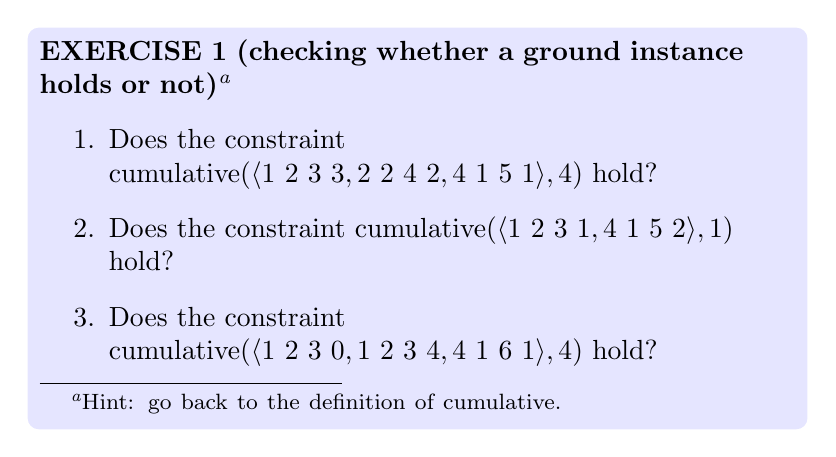
\begin{tikzpicture}
[information text/.style={rounded corners,inner sep=1ex}]
\draw
node[right,text width=9.6cm,information text,fill=blue!10]
{{\bf EXERCISE 1 (checking whether a ground instance holds or not)\footnote{Hint: go back to the definition of \ctrrefself{cumulative}.}}
\begin{enumerate}
\item
Does the constraint
\ctrrefself{cumulative}$(\langle 1~2~3~3, 2~2~4~2, 4~1~5~1\rangle, 4)$ hold?
\item
Does the constraint
\ctrrefself{cumulative}$(\langle 1~2~3~1, 4~1~5~2\rangle, 1)$ hold?
\item
Does the constraint
\ctrrefself{cumulative}$(\langle 1~2~3~0, 1~2~3~4, 4~1~6~1\rangle, 4)$ hold?
\end{enumerate}
};
\end{tikzpicture}
}
~\\

% Hint:
% reason first on the two highest tasks and then on the two smallest tasks.
{\small
\exercisecaption{\ctrrefself{cumulative}: finding all solutions}
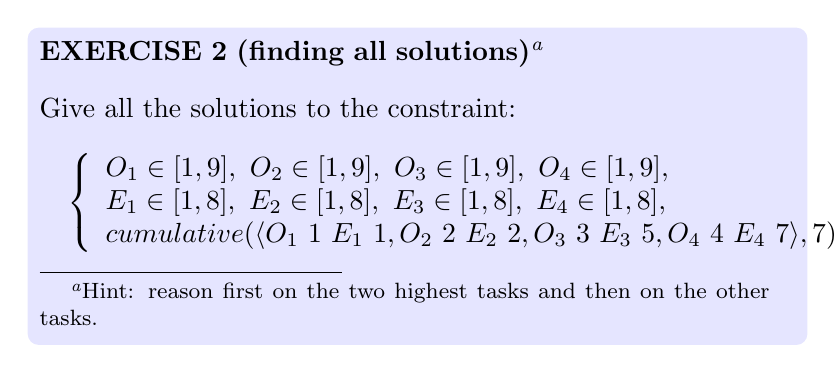
\begin{tikzpicture}
[information text/.style={rounded corners,inner sep=1ex}]
\draw[xshift=-3cm,yshift=3.3cm]
node[right,text width=9.6cm,information text,fill=blue!10]
{{\bf EXERCISE 2 (finding all solutions)\footnote{Hint: reason first on the two highest tasks and then on the other tasks.}}\\
\vspace{0.3cm}
Give all the solutions to the constraint:\\~\\
\hspace*{1em}$\left\{
\begin{array}{l}
O_1\in[1,9], ~O_2\in[1,9], ~O_3\in[1,9], ~O_4\in[1,9],\\
E_1\in[1,8], ~E_2\in[1,8], ~E_3\in[1,8], ~E_4\in[1,8],\\
\constraint{cumulative}(\langle O_1~1~E_1~1, O_2~2~E_2~2, O_3~3~E_3~5, O_4~4~E_4~7\rangle,7).\\
\end{array}
\right.$\\~\\
};
\end{tikzpicture}
}
~\\

{\small
\renewcommand\theenumi {\bf\Alph{enumi}}
\begin{tikzpicture}
[information text/.style={rounded corners,inner sep=1ex}]
\draw
node[right,text width=6cm,information text,fill=red!10]
{{\bf SOLUTION TO EXERCISE 1}\\
\begin{enumerate}
\item
\emph{No, since the first and second tasks overlap at time point $2$
and use up to $3+2$ resource units which exceeds the resource capacity $4$.}\\
\item
\emph{No, since the second task uses $2$ resource units,
while the resource capacity is $1$.}
\item
\emph{No, since for the third task the origin plus the duration is different
from the end} ($4+1\neq 6$).
\end{enumerate}
};
\begin{scope}[xshift=7.2cm,yshift=0.3cm,scale=0.30]
\draw[step=1cm,gray,very thin] (0,0) grid (5,4);
\filldraw[fill=MyRhodamine!20!white, draw=black!65, line width=0.6pt] (1,0) rectangle (3,3);
\filldraw[fill=black, draw=black] (1,0) rectangle (1.25,0.25);
\coordinate [label=left:\textcolor{MyRhodamine}{{\scriptsize$\mathbf{1}$}}] (T1) at (2.7,1.5);
\filldraw[fill=MyRedOrange!20!white, draw=black!65, line width=0.6pt] (2,3) rectangle (3,5);
\filldraw[fill=black, draw=black] (2,3) rectangle (2.25,3.25);
\filldraw[fill=MyRedOrange!20!white, draw=black!65, line width=0.6pt] (3,0) rectangle (4,2);
\coordinate [label=left:\textcolor{MyRedOrange}{{\scriptsize$\mathbf{2}$}}] (T2) at (4.15,1);
\filldraw[fill=MyPineGreen!20!white, draw=black!65, line width=0.6pt] (4,0) rectangle (5,4);
\filldraw[fill=black, draw=black] (4,0) rectangle (4.25,0.25);
\coordinate [label=left:\textcolor{MyPineGreen}{{\scriptsize$\mathbf{3}$}}] (T4) at (5.15,2.0);
\foreach \x in {1,2,3,4,5}
\draw[draw=black,line width=0.5pt] (\x,0) -- (\x,0.2);
\foreach \x in {1,2,3,4,5}
\coordinate [label=left:{\scriptsize$\x$}] (X) at (0.5+\x,-0.5);
\foreach \y in {1,2,3,4}
\draw[draw=black,line width=0.5pt] (0,\y) -- (0.2,\y);
\foreach \y in {1,2,3,4}
\coordinate [label=left:{\scriptsize$\y$}] (Y) at (-0.1,\y+0.1);
\draw[draw=red!70,line width=2.0pt] (0,4) -- (5,4);
\coordinate [label=left:{\scriptsize(A)}] (L) at (7.0,4.6);
\draw[draw=black,line width=0.8pt,->] (0,0) -- (6.75,0);
\draw[draw=black,line width=0.8pt,->] (0,0) -- (0,5.25);
\end{scope}
\begin{scope}[xshift=7.2cm,yshift=-0.9cm,scale=0.30]
\draw[step=1cm,gray,very thin] (0,0) grid (5,1);
\filldraw[fill=MyRhodamine!20!white, draw=black!65, line width=0.6pt] (1,0) rectangle (3,1);
\filldraw[fill=black, draw=black] (1,0) rectangle (1.25,0.25);
\coordinate [label=left:\textcolor{MyRhodamine}{{\scriptsize$\mathbf{1}$}}] (T1) at (2.65,0.55);
\filldraw[fill=MyRedOrange!20!white, draw=black!65, line width=0.6pt] (3,0) rectangle (4,2);
\filldraw[fill=black, draw=black] (3,0) rectangle (3.25,0.25);
\coordinate [label=left:\textcolor{MyRedOrange}{{\scriptsize$\mathbf{2}$}}] (T2) at (4.15,0.55);
\foreach \x in {1,2,3,4,5}
\draw[draw=black,line width=0.5pt] (\x,0) -- (\x,0.2);
\foreach \x in {1,2,3,4,5}
\coordinate [label=left:{\scriptsize$\x$}] (X) at (0.5+\x,-0.5);
\foreach \y in {1}
\draw[draw=black,line width=0.5pt] (0,\y) -- (0.2,\y);
\foreach \y in {1}
\coordinate [label=left:{\scriptsize$\y$}] (Y) at (-0.1,\y+0.1);
\draw[draw=red!70,line width=2.0pt] (0,1) -- (5,1);
\coordinate [label=left:{\scriptsize(B)}] (L) at (7.0,1.6);
\draw[draw=black,line width=0.8pt,->] (0,0) -- (6.75,0);
\draw[draw=black,line width=0.8pt,->] (0,0) -- (0,2.25);
\end{scope}
\end{tikzpicture}
}
~\\

{\small
\begin{tikzpicture}
[information text/.style={rounded corners,inner sep=1ex}]
\draw
node[right,text width=7.6cm,information text,fill=red!10]
{{\bf SOLUTION TO EXERCISE 2}\\
\hspace*{0.15cm}(\emph{nested disjunctions})
\begin{enumerate}
\item
\emph{Since we have a resource limit of $7$ the third task (of height $5$)
cannot overlap the fourth task (of height $7$). Since there is no slack on
the time axis (i.e., the difference between the latest end of the third and
fourth tasks and their earliest start is equal to the sum of their durations,
$8-1=3+4$), this leads to the two configurations shown on the right.}
\item
\emph{Since there is no available space on top of the fourth task,
the first and second tasks have to be put on top of the third task.
Since on top of the third task we only have a capacity of $2$
the first and second tasks cannot overlap. Since there is no
remaining slack on the time axis this leads to the two configurations
shown on the right.}
\item
\emph{Combining the two previous observations together leads to
the four solutions shown below.}
\end{enumerate}
};
\begin{scope}[xshift=8cm,yshift=1.4cm,scale=0.20]
\filldraw[fill=MyPineGreen!20!white, draw=black!65, line width=0.6pt] (1,0) rectangle (4,5);
\coordinate [label=left:\textcolor{MyPineGreen}{{\scriptsize$\mathbf{3}$}}] (T4) at (3.5,2.5);
\filldraw[fill=MyCornflowerBlue!20!white, draw=black!65, line width=0.6pt] (4,0) rectangle (8,7);
\coordinate [label=left:\textcolor{MyCornflowerBlue}{{\scriptsize$\mathbf{4}$}}] (T4) at (7.0,3.5);
\draw[draw=red!70,line width=1.0pt] (1,7) -- (8,7);
\draw[draw=red!70,line width=1.0pt] (1,0) -- (1,7);
\draw[draw=red!70,line width=1.0pt] (8,0) -- (8,7);
\end{scope}
\begin{scope}[xshift=8cm,yshift=-0.2cm,scale=0.20]
\filldraw[fill=MyPineGreen!20!white, draw=black!65, line width=0.6pt] (5,0) rectangle (8,5);
\filldraw[fill=MyCornflowerBlue!20!white, draw=black!65, line width=0.6pt] (1,0) rectangle (5,7);
\coordinate [label=left:\textcolor{MyPineGreen}{{\scriptsize$\mathbf{3}$}}] (T4) at (7.5,2.5);
\coordinate [label=left:\textcolor{MyCornflowerBlue}{{\scriptsize$\mathbf{4}$}}] (T4) at (4,3.5);
\draw[draw=red!70,line width=1.0pt] (1,7) -- (8,7);
\draw[draw=red!70,line width=1.0pt] (1,0) -- (1,7);
\draw[draw=red!70,line width=1.0pt] (8,0) -- (8,7);
\end{scope}
\begin{scope}[xshift=8.4cm,yshift=-2.1cm,scale=0.20]
\filldraw[fill=MyPineGreen!20!white, draw=black!65, line width=0.6pt] (1,0) rectangle (4,5);
\coordinate [label=left:\textcolor{MyPineGreen}{{\scriptsize$\mathbf{3}$}}] (T4) at (3.5,2.5);
\filldraw[fill=MyRhodamine!20!white, draw=black!65, line width=0.6pt] (1,5) rectangle (2,6);
\coordinate [label=left:\textcolor{MyRhodamine}{{\scriptsize$\mathbf{1}$}}] (T1) at (2.5,5.5);
\filldraw[fill=MyRedOrange!20!white, draw=black!65, line width=0.6pt] (2,5) rectangle (4,7);
\coordinate [label=left:\textcolor{MyRedOrange}{{\scriptsize$\mathbf{2}$}}] (T2) at (3.9,6);
\draw[draw=red!70,line width=1.0pt] (1,7) -- (4,7);
\draw[draw=red!70,line width=1.0pt] (1,0) -- (1,7);
\draw[draw=red!70,line width=1.0pt] (4,0) -- (4,7);
\end{scope}
\begin{scope}[xshift=8.4cm,yshift=-3.7cm,scale=0.20]
\filldraw[fill=MyPineGreen!20!white, draw=black!65, line width=0.6pt] (1,0) rectangle (4,5);
\coordinate [label=left:\textcolor{MyPineGreen}{{\scriptsize$\mathbf{3}$}}] (T4) at (3.5,2.5);
\filldraw[fill=MyRhodamine!20!white, draw=black!65, line width=0.6pt] (3,5) rectangle (4,6);
\coordinate [label=left:\textcolor{MyRhodamine}{{\scriptsize$\mathbf{1}$}}] (T1) at (4.5,5.5);
\filldraw[fill=MyRedOrange!20!white, draw=black!65, line width=0.6pt] (1,5) rectangle (3,7);
\coordinate [label=left:\textcolor{MyRedOrange}{{\scriptsize$\mathbf{2}$}}] (T2) at (3,6);
\draw[draw=red!70,line width=1.0pt] (1,7) -- (4,7);
\draw[draw=red!70,line width=1.0pt] (1,0) -- (1,7);
\draw[draw=red!70,line width=1.0pt] (4,0) -- (4,7);
\end{scope}
\begin{scope}[xshift=4.5cm,yshift=-5.7cm]
\node [single arrow, single arrow tip angle=135, single arrow head extend=1cm, draw=MyCornflowerBlue, line width=2pt,fill=MyYellowlight, single arrow, shape border rotate=270, text width=6.5cm, label=above:{{{\color{MyCornflowerBlue}\bf the four solutions}}}]
{{\tiny~~~~~~$\langle O_1 D_1 E_1 H_1, O_2 D_2 E_2 H_2, O_3 D_3 E_3 H_3, O_4 D_4 E_4 H_4\rangle$}\\
~\ding{172}~~$(\langle	{\color{MyRhodamine}\mathbf{1~1~2~1}},~~
{\color{MyRedOrange}\mathbf{2~2~4~2}},~~
{\color{MyPineGreen}\mathbf{1~3~4~5}},~~
{\color{MyCornflowerBlue}\mathbf{4~4~8~7}}\rangle)$\\
~\ding{173}~~$(\langle 	{\color{MyRhodamine}\mathbf{3~1~4~1}},~~
{\color{MyRedOrange}\mathbf{1~2~3~2}},~~
{\color{MyPineGreen}\mathbf{1~3~4~5}},~~
{\color{MyCornflowerBlue}\mathbf{4~4~8~7}}\rangle)$\\
~\ding{174}~~$(\langle	{\color{MyRhodamine}\mathbf{5~1~6~1}},~~
{\color{MyRedOrange}\mathbf{6~2~8~2}},~~
{\color{MyPineGreen}\mathbf{5~3~8~5}},~~
{\color{MyCornflowerBlue}\mathbf{1~4~5~7}}\rangle)$\\
~\ding{175}~~$(\langle	{\color{MyRhodamine}\mathbf{7~1~8~1}},~~
{\color{MyRedOrange}\mathbf{5~2~7~2}},~~
{\color{MyPineGreen}\mathbf{5~3~8~5}},~~
{\color{MyCornflowerBlue}\mathbf{1~4~5~7}}\rangle)$};
\end{scope}
\begin{scope}[xshift=0.5cm,yshift=-10.4cm,scale=0.30]
\draw[step=1cm,gray,very thin] (0,0) grid (10,7);
\filldraw[fill=MyRhodamine!20!white, draw=black!65, line width=0.6pt] (1,5) rectangle (2,6);
\filldraw[fill=black, draw=black] (1,5) rectangle (1.25,5.25);
\coordinate [label=left:\textcolor{MyRhodamine}{{\scriptsize$\mathbf{1}$}}] (T1) at (2.1,5.5);
\filldraw[fill=MyRedOrange!20!white, draw=black!65, line width=0.6pt] (2,5) rectangle (4,7);
\filldraw[fill=black, draw=black] (2,5) rectangle (2.25,5.25);
\coordinate [label=left:\textcolor{MyRedOrange}{{\scriptsize$\mathbf{2}$}}] (T2) at (3.5,6);
\filldraw[fill=MyPineGreen!20!white, draw=black!65, line width=0.6pt] (1,0) rectangle (4,5);
\filldraw[fill=black, draw=black] (1,0) rectangle (1.25,0.25);
\coordinate [label=left:\textcolor{MyPineGreen}{{\scriptsize$\mathbf{3}$}}] (T4) at (3,2.5);
\filldraw[fill=MyCornflowerBlue!20!white, draw=black!65, line width=0.6pt] (4,0) rectangle (8,7);
\filldraw[fill=black, draw=black] (4,0) rectangle (4.25,0.25);
\coordinate [label=left:\textcolor{MyCornflowerBlue}{{\scriptsize$\mathbf{4}$}}] (T4) at (6.5,3.5);
\foreach \x in {1,2,3,4,5,6,7,8,9,10}
\draw[draw=black,line width=0.5pt] (\x,0) -- (\x,0.2);
\foreach \x in {1,2,3,4,5,6,7,8}
\coordinate [label=left:{\scriptsize$\x$}] (X) at (0.5+\x,-0.5);
\foreach \y in {1,2,3,4,5,6,7}
\draw[draw=black,line width=0.5pt] (0,\y) -- (0.2,\y);
\foreach \y in {1,2,3,4,5,6,7}
\coordinate [label=left:{\scriptsize$\y$}] (Y) at (-0.1,\y+0.1);
\draw[draw=red!70,line width=2.0pt] (0,7) -- (10,7);
\coordinate [label=left:\ding{172}] (L) at (10.30,6.5);
\draw[draw=red!70,line width=1.0pt] (1,0) -- (1,7);
\draw[draw=red!70,line width=1.0pt] (8,0) -- (8,7);
\draw[draw=black,line width=0.8pt,->] (0,0) -- (10.75,0);
\draw[draw=black,line width=0.8pt,->] (0,0) -- (0,7.75);
\end{scope}
\begin{scope}[xshift=5.70cm,yshift=-10.4cm,scale=0.30]
\draw[step=1cm,gray,very thin] (0,0) grid (10,7);
\filldraw[fill=MyRhodamine!20!white, draw=black!65, line width=0.6pt] (3,5) rectangle (4,6);
\filldraw[fill=black, draw=black] (3,5) rectangle (3.25,5.25);
\coordinate [label=left:\textcolor{MyRhodamine}{{\scriptsize$\mathbf{1}$}}] (T1) at (4.1,5.5);
\filldraw[fill=MyRedOrange!20!white, draw=black!65, line width=0.6pt] (1,5) rectangle (3,7);
\filldraw[fill=black, draw=black] (1,5) rectangle (1.25,5.25);
\coordinate [label=left:\textcolor{MyRedOrange}{{\scriptsize$\mathbf{2}$}}] (T2) at (2.5,6);
\filldraw[fill=MyPineGreen!20!white, draw=black!65, line width=0.6pt] (1,0) rectangle (4,5);
\filldraw[fill=black, draw=black] (1,0) rectangle (1.25,0.25);
\coordinate [label=left:\textcolor{MyPineGreen}{{\scriptsize$\mathbf{3}$}}] (T4) at (3,2.5);
\filldraw[fill=MyCornflowerBlue!20!white, draw=black!65, line width=0.6pt] (4,0) rectangle (8,7);
\filldraw[fill=black, draw=black] (4,0) rectangle (4.25,0.25);
\coordinate [label=left:\textcolor{MyCornflowerBlue}{{\scriptsize$\mathbf{4}$}}] (T4) at (6.5,3.5);
\foreach \x in {1,2,3,4,5,6,7,8,9,10}
\draw[draw=black,line width=0.5pt] (\x,0) -- (\x,0.2);
\foreach \x in {1,2,3,4,5,6,7,8}
\coordinate [label=left:{\scriptsize$\x$}] (X) at (0.5+\x,-0.5);
\foreach \y in {1,2,3,4,5,6,7}
\draw[draw=black,line width=0.5pt] (0,\y) -- (0.2,\y);
\foreach \y in {1,2,3,4,5,6,7}
\coordinate [label=left:{\scriptsize$\y$}] (Y) at (-0.1,\y+0.1);
\draw[draw=red!70,line width=2.0pt] (0,7) -- (10,7);
\coordinate [label=left:\ding{173}] (L) at (10.30,6.5);
\draw[draw=red!70,line width=1.0pt] (1,0) -- (1,7);
\draw[draw=red!70,line width=1.0pt] (8,0) -- (8,7);
\draw[draw=black,line width=0.8pt,->] (0,0) -- (10.75,0);
\draw[draw=black,line width=0.8pt,->] (0,0) -- (0,7.75);
\end{scope}
\begin{scope}[xshift=0.5cm,yshift=-13.1cm,scale=0.30]
\draw[step=1cm,gray,very thin] (0,0) grid (10,7);
\filldraw[fill=MyRhodamine!20!white, draw=black!65, line width=0.6pt] (5,5) rectangle (6,6);
\filldraw[fill=black, draw=black] (5,5) rectangle (5.25,5.25);
\coordinate [label=left:\textcolor{MyRhodamine}{{\scriptsize$\mathbf{1}$}}] (T1) at (6.1,5.5);
\filldraw[fill=MyRedOrange!20!white, draw=black!65, line width=0.6pt] (6,5) rectangle (8,7);
\filldraw[fill=black, draw=black] (6,5) rectangle (6.25,5.25);
\coordinate [label=left:\textcolor{MyRedOrange}{{\scriptsize$\mathbf{2}$}}] (T2) at (7.5,6);
\filldraw[fill=MyPineGreen!20!white, draw=black!65, line width=0.6pt] (5,0) rectangle (8,5);
\filldraw[fill=black, draw=black] (5,0) rectangle (5.25,0.25);
\coordinate [label=left:\textcolor{MyPineGreen}{{\scriptsize$\mathbf{3}$}}] (T4) at (7,2.5);
\filldraw[fill=MyCornflowerBlue!20!white, draw=black!65, line width=0.6pt] (1,0) rectangle (5,7);
\filldraw[fill=black, draw=black] (1,0) rectangle (1.25,0.25);
\coordinate [label=left:\textcolor{MyCornflowerBlue}{{\scriptsize$\mathbf{4}$}}] (T4) at (3.5,3.5);
\foreach \x in {1,2,3,4,5,6,7,8,9,10}
\draw[draw=black,line width=0.5pt] (\x,0) -- (\x,0.2);
\foreach \x in {1,2,3,4,5,6,7,8}
\coordinate [label=left:{\scriptsize$\x$}] (X) at (0.5+\x,-0.5);
\foreach \y in {1,2,3,4,5,6,7}
\draw[draw=black,line width=0.5pt] (0,\y) -- (0.2,\y);
\foreach \y in {1,2,3,4,5,6,7}
\coordinate [label=left:{\scriptsize$\y$}] (Y) at (-0.1,\y+0.1);
\draw[draw=red!70,line width=2.0pt] (0,7) -- (10,7);
\coordinate [label=left:\ding{174}] (L) at (10.30,6.5);
\draw[draw=red!70,line width=1.0pt] (1,0) -- (1,7);
\draw[draw=red!70,line width=1.0pt] (8,0) -- (8,7);
\draw[draw=black,line width=0.8pt,->] (0,0) -- (10.75,0);
\draw[draw=black,line width=0.8pt,->] (0,0) -- (0,7.75);
\end{scope}
\begin{scope}[xshift=5.70cm,yshift=-13.1cm,scale=0.30]
\draw[step=1cm,gray,very thin] (0,0) grid (10,7);
\filldraw[fill=MyRhodamine!20!white, draw=black!65, line width=0.6pt] (7,5) rectangle (8,6);
\filldraw[fill=black, draw=black] (7,5) rectangle (7.25,5.25);
\coordinate [label=left:\textcolor{MyRhodamine}{{\scriptsize$\mathbf{1}$}}] (T1) at (8.1,5.5);
\filldraw[fill=MyRedOrange!20!white, draw=black!65, line width=0.6pt] (5,5) rectangle (7,7);
\filldraw[fill=black, draw=black] (5,5) rectangle (5.25,5.25);
\coordinate [label=left:\textcolor{MyRedOrange}{{\scriptsize$\mathbf{2}$}}] (T2) at (6.5,6);
\filldraw[fill=MyPineGreen!20!white, draw=black!65, line width=0.6pt] (5,0) rectangle (8,5);
\filldraw[fill=black, draw=black] (5,0) rectangle (5.25,0.25);
\coordinate [label=left:\textcolor{MyPineGreen}{{\scriptsize$\mathbf{3}$}}] (T4) at (7,2.5);
\filldraw[fill=MyCornflowerBlue!20!white, draw=black!65, line width=0.6pt] (1,0) rectangle (5,7);
\filldraw[fill=black, draw=black] (1,0) rectangle (1.25,0.25);
\coordinate [label=left:\textcolor{MyCornflowerBlue}{{\scriptsize$\mathbf{4}$}}] (T4) at (3.5,3.5);
\foreach \x in {1,2,3,4,5,6,7,8,9,10}
\draw[draw=black,line width=0.5pt] (\x,0) -- (\x,0.2);
\foreach \x in {1,2,3,4,5,6,7,8}
\coordinate [label=left:{\scriptsize$\x$}] (X) at (0.5+\x,-0.5);
\foreach \y in {1,2,3,4,5,6,7}
\draw[draw=black,line width=0.5pt] (0,\y) -- (0.2,\y);
\foreach \y in {1,2,3,4,5,6,7}
\coordinate [label=left:{\scriptsize$\y$}] (Y) at (-0.1,\y+0.1);
\draw[draw=red!70,line width=2.0pt] (0,7) -- (10,7);
\coordinate [label=left:\ding{175}] (L) at (10.30,6.5);
\draw[draw=red!70,line width=1.0pt] (1,0) -- (1,7);
\draw[draw=red!70,line width=1.0pt] (8,0) -- (8,7);
\draw[draw=black,line width=0.8pt,->] (0,0) -- (10.75,0);
\draw[draw=black,line width=0.8pt,->] (0,0) -- (0,7.75);
\end{scope}
\end{tikzpicture}
}
\end{ctrdesc}


\pagestyle{headings}
\begin{appendix}
\chapter{Legend for the Description}\label{chap:legend}

This section provides the list of \emph{restrictions}, of \emph{arc generators}, of \emph{graph parameters} and of \emph{set generators} sorted in alphabetic order with the page where they are defined.

\end{appendix}
\backmatter


%%% Local Variables: 
%%% mode: latex
%%% TeX-master: "catalog"
%%% End: 


\cleardoublepage
\markboth{REFERENCES}{REFERENCES}
\phantomsection
\addcontentsline{toc}{chapter}{Bibliography}
\bibliographystyle{plain}
\bibliography{catalog}

\cleardoublepage
\markboth{INDEX}{INDEX}
\phantomsection
\addcontentsline{toc}{chapter}{Index}
\printindex
\end{document}

%%% Local Variables: 
%%% mode: latex
%%% TeX-master: t
%%% End: 
